\documentclass[12pt, a4paper, oneside]{ctexbook}
\usepackage{amsmath, amsthm, amssymb, bm, graphicx, hyperref, mathrsfs, diagbox, color, tikz}
\usetikzlibrary{positioning, arrows.meta}

\newcommand{\Var}{\operatorname{Var}}
\newcommand{\Cov}{\operatorname{Cov}}
\newcommand{\dx}{\operatorname{dx}}
\newcommand{\dt}{\operatorname{dt}}
\newcommand{\dbx}{\operatorname{d}\mathbf{x}}
\newcommand{\dy}{\operatorname{dy}}
\newcommand{\Vol}{\operatorname{Vol}}
\newcommand{\bmu}{\bm{\mu}}
\newcommand{\bK}{\mathbf{K}}
\newcommand{\bx}{\mathbf{x}}
\newcommand{\Tr}{\text{Tr}}

\title{{\Huge{\textbf{EE142 \\ Fundamentals of Information Theory}}}\\Lecture notes}
\author{Zhou Shouchen\\ 2021533042 \\ \href{https://github.com/zsc2003/ShanghaiTech-EE142}{\LaTeX{} source code on GitHub}}
\date{\today}
\linespread{1.4}
\newtheorem{theorem}{定理}[section]
\newtheorem{definition}[theorem]{定义}
\newtheorem{lemma}[theorem]{引理}
\newtheorem{corollary}[theorem]{推论}
\newtheorem{example}[theorem]{例}
\newtheorem{proposition}[theorem]{命题}

\begin{document}

\maketitle

% -------------------- chapters --------------------
\pagenumbering{Roman}
\setcounter{page}{1}
\tableofcontents
\newpage
\setcounter{page}{1}
\pagenumbering{arabic}

\chapter{Summary}


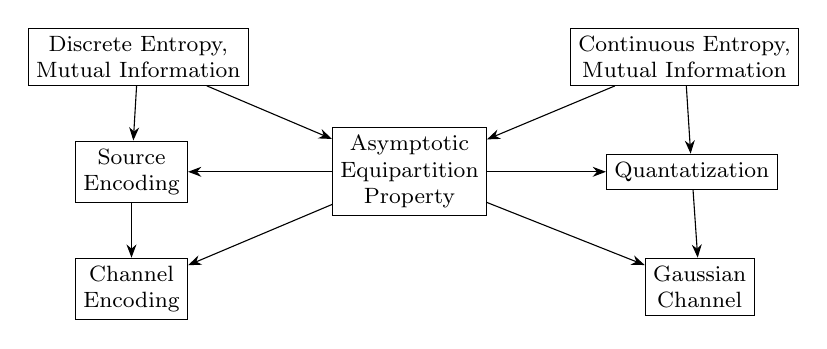
\begin{tikzpicture}[
    every node/.style={rectangle, draw, align=center},
    arrow/.style={-Stealth}
]
\centering
\footnotesize
\node (AEP) {Asymptotic \\ Equipartition \\ Property};
\node (discrete) [above left=15pt and 30pt of AEP] {Discrete Entropy, \\ Mutual Information};
\node (sourceencoding) [left=52pt of AEP] {Source \\ Encoding};
\node (channelencoding) [below left=15pt and 52pt of AEP] {Channel \\ Encoding};

\node (continuous) [above right=15pt and 30pt of AEP] {Continuous Entropy, \\ Mutual Information};
\node (quantatization) [right=43pt of AEP] {Quantatization};
\node (Gaussianchannel) [below right=15pt and 57pt of AEP] {Gaussian \\ Channel};

\draw [arrow] (discrete) -- (AEP);
\draw [arrow] (continuous) -- (AEP);
\draw [arrow] (AEP) -- (channelencoding);
\draw [arrow] (AEP) -- (sourceencoding);
\draw [arrow] (AEP) -- (Gaussianchannel);
\draw [arrow] (AEP) -- (quantatization);
\draw [arrow] (discrete) -- (sourceencoding);
\draw [arrow] (sourceencoding) -- (channelencoding);
\draw [arrow] (continuous) -- (quantatization);
\draw [arrow] (quantatization) -- (Gaussianchannel);
\end{tikzpicture}

A.E.P. 将所有的章节连接起来.

主要围绕香农三大定理展开: (注意成立的条件! 所有事情要满足其条件才行!)
\begin{enumerate}
\item Lossless Source Coding Theorem (\textcolor{red}{前提: $x^n\stackrel{i.i.d.}{\sim} p(x)$})
$$L^* = H(X)$$

\item Channel Coding Theorem (\textcolor{red}{前提: Memoryless Channel})
$$C^* = \max_{p(x)}I(X;Y)$$

\item Rate Distortion Theorem (\textcolor{red}{前提: $x^n\stackrel{i.i.d.}{\sim} p(x)$})
$$R(D) = \min_{p(x), \mathbb{E}(X)\leq p^2}I(X;\hat{X})$$
\end{enumerate}

Some interesting topics but not covered in class:
$\S 11.3$ Universal Source Coding, $\S 11.10$ Fisher Information, $\S 15.10$ General Multiterminal Networks.

$\ldots\ldots\ldots\ldots$ A lot of interesting topics $\ldots\ldots\ldots\ldots$
\chapter{Entropy, Relative Entropy, Mutual Information}
Book Chapter2. (P39)

$\log x$若无特殊说明, 默认为$\log_2 x$, $0\log 0=0$.

离散型随机变量$\mathcal{X}$看作是有限的, i.e. $|\mathcal{X}|<+\infty$.

\section{Gaussian Channel}
一个信号 $x(t)$ 的能量和功率为
\begin{align*}
E &= \int_{-\infty}^{\infty} x^2(t) \dt \\
P &= \lim_{T\to\infty} \dfrac{1}{T}\int_{-\frac{T}{2}}^{\frac{T}{2}} x^2(t) \dt
\end{align*}
当传输为离散时, 采样点为 $X_1,\ldots, X_n\stackrel{i.i.d.}{\sim} X$, 由大数定理可得:
$$P = \lim_{T\to\infty} \dfrac{1}{T}\sum_{n=-\frac{T}{2}}^{\frac{T}{2}} X_i^2\to \mathbb{E}(X^2)$$
信道在传输信号时有传输功率 $P$ 的限制. 所以我们可以用 $\mathbb{E}(X^2)\leq P$ 作为信号的传输功率限制. 因为平移不会改变信息熵, 所以不妨设$X$的均值为$0$以减少能量的浪费, 此时约束变为 $\Var(X)\leq P$.
\begin{figure}[htbp]
    \centering
    \includegraphics[width=0.4\textwidth]{./figures/chapter7/Gaussian_channel.png}
\end{figure}

高斯信道如下图所示. 其中$X$为信道的输入, 传输过程中有噪声$Z \sim \mathcal{N}(0, N)$, 且$X\perp Z$. 信道的输出为$Y = X + Z$. 高斯信道又叫 Additive White Gaussian Noise (AWGN) 信道.

由于信道容量$C$为每次可靠传输的bit数, 所以$N=0$时$C=+\infty$. 若$X$传输时没有功率限制, 则$C=+\infty$. 但是在考虑真实的高斯信道时加上$\Var(X)\leq P$的限制.

由上一章可知, Gaussian的方差为$\sigma^2$时的熵为$h(X) = \dfrac{1}{2}\ln(2\pi e \sigma^2)$ nats. 所以当 $X\sim \mathcal{N}(0, P)$ 时, $Y\sim \mathcal{N}(0, P+N)$, $Y|X\sim \mathcal{N}(X, N)$, 此时有
$$I(X;Y) = h(Y) - h(Y|X) = \dfrac{1}{2}\ln\left(1+\dfrac{P}{N}\right) \text{ nats}$$
后面我们证明这其实就是高斯信道的信道容量.

\begin{example}
A non-optimal example: Let $X=\begin{cases}
\sqrt{P}, &\text{w.p. } \dfrac{1}{2} \\
-\sqrt{P}, &\text{w.p. } \dfrac{1}{2}
\end{cases}$. $X$有 $\mathbb{E}(X)=0, \Var(X)=P$.
若取Decoder为$\hat{X}=\arg\max\limits_{\hat{X}}\|Y-\hat{X}\|^2$, 则有$\hat{X}=\begin{cases}
\sqrt{P}, &\text{if } Y\geq 0 \\
-\sqrt{P}, &\text{if } Y<0
\end{cases}$. 此时有错误概率
\begin{align*}
P_e &= \Pr(\hat{X}\neq X) = \Pr(Y<0|X=\sqrt{P})\cdot\Pr(X=\sqrt{P}) + \Pr(Y\geq 0|X=-\sqrt{P})\cdot\Pr(X=-\sqrt{P}) \\
&= \dfrac{1}{2}\Pr(Y<0|X=\sqrt{P}) + \dfrac{1}{2}\Pr(Y\geq 0|X=-\sqrt{P}) = \dfrac{1}{2}\Pr(Z>\sqrt{P}) + \dfrac{1}{2}\Pr(Z<-\sqrt{P}) \\
&= \dfrac{1}{2}\left(1-\Phi\left(\dfrac{\sqrt{P}}{\sqrt{N}}\right)\right) + \dfrac{1}{2}\Phi\left(\dfrac{\sqrt{P}}{\sqrt{N}}\right) \\
&= \dfrac{1}{2}\left(1-\Phi\left(\dfrac{\sqrt{P}}{\sqrt{N}}\right)\right) + \dfrac{1}{2}\left(1-\Phi\left(\dfrac{\sqrt{P}}{\sqrt{N}}\right)\right) \\
&= 1-\Phi\left(\sqrt{\dfrac{P}{N}}\right)
\end{align*}
\end{example}
和先前证明信道容量时的方法类似, 我们通过Achievability和Converse来证明信道容量. 我们先通过填充球理论 sphere packing(本质还是AEP)来直观感受:
\begin{figure}[htbp]
    \centering
    \includegraphics[width=0.5\textwidth]{./figures/chapter7/sphere_picking.png}
\end{figure}

如上图所示, 假设每一个小球的球心为一个codeword, 球的范围为可以decode到该codeword的所有码字(jointly AEP). 假设这些小球的半径为$r$, 则一个$n$为球的体积可以写为$\Vol=C_nr^n$. 由于 noise的方差为$N$, 所以小球的半径为 $\sqrt{n(n+\epsilon)}$, 而$Y$的方差为$\mathbb{E}(Y^2)=\mathbb{E}((X+Z)^2)=\mathbb{E}(X^2)+\mathbb{E}(Z^2)=P+N$, 所以整个大球的半径为$\sqrt{n(P+N)}$. 因此最多有 $\dfrac{C_n(\sqrt{n(P+N)})^n}{C_n(\sqrt{n(n+\epsilon)})^n}=\left(1+\dfrac{P}{N}\right)^{\frac{1}{2}}$ 个小球. 所以rate of the code(小球数量需要的bit数) is $\log \left(1+\dfrac{P}{N}\right)^{\frac{1}{2}}=\dfrac{1}{2}\log\left(1+\dfrac{P}{N}\right)$.

关于大球的半径大小: typical set的大小为$\Vol\left(A_{\epsilon}^{(n)}(f_Y)\right)=2^{n(H(Y))}\leq 2^{n(\frac{1}{2}\log(2\pi e (P+N)))}$, 所以半径取 $\sqrt{n(P+N)}$. 小球的半径同理.

严谨证明:
1. 可达性证明: 大致和先前证明信道容量的方法类似, 要证明$\forall R<C=I(X;Y)$时, 发生错误的概率 $P_e^{(n)}\to 0$.

通过构建码本, $X_i(w)$ 表示 码字$w$的第$i$个bit. 其中 $X_i(w)\stackrel{i.i.d.}{\sim} \mathcal{N}(0, P-\epsilon)$.

和先前一样, W.L.O.G. 令w=1, 则 $P_e^{(n)}=\Pr\left(\hat{W}\neq 1|W=1\right)$, 然后分类讨论不符合要求的情况即可. \textcolor{red}{不同之处: 增加了$E_0:\dfrac{1}{n}\sum\limits_{j=1}^n X_j(1)>P$(不满足功率约束限制)的情况}.

摆烂了, 放图片了.
\begin{figure}[htbp]
    \centering
    \includegraphics[width=1.25\textwidth]{./figures/chapter7/achievability.png}
\end{figure}

想要$P_e^{(n)}\to 0$, 则需要$2^{-n(I(X;Y)-R-3\epsilon)}\to 0$, i.e. $R<I(X;Y)-3\epsilon$. 这里所有提到的$I(X;Y)$都是$\max\limits_{p(x)}I(X;Y)=\frac{1}{2}\log \left(1+\frac{P}{N}\right)$.

2. Converse proof: \\
证明$\forall R>C=\frac{1}{2}\log\left(1+\frac{P}{N}\right)$时, $P_e^{(n)}\not\to 0$ with $\mathbb{E}(X^2)\leq P$. \\
同样要用 Fano's Inequality, 对于信息传递的Markov Chain $W\to X\to Y\to \hat{W}$, 有
$$H(W|\hat{W})\leq 1 + P_e^{(n)}\log 2^{nR} = 1 + P_e^{(n)}nR \triangleq n\epsilon_n$$

\begin{figure}[htbp]
    \centering
    \includegraphics[width=1.25\textwidth]{./figures/chapter7/converse.png}
\end{figure}
$$R\leq \dfrac{1}{2}\log\left(1+\dfrac{P}{N}\right)+\epsilon_n=\dfrac{1}{2}\log\left(1+\dfrac{P}{N}\right)+\dfrac{1}{n}+P_e^{(n)}R$$
当$R>C=\dfrac{1}{2}\log\left(1+\dfrac{P}{N}\right)$时, 有$\dfrac{1}{n}+P_e^{(n)}R>0$, 由于$n,R$均为常数, 所以一定有$P_e^{(n)}\not\to 0$.
\section{Relative Entropy and Mutual Information}
概率论衡量两个变量相关程度(概率论方法):
$$\rho_{X,Y}=\dfrac{\Cov(X,Y)}{\sqrt{\Var(X)\Var(Y)}}\in[-1,1]$$
只能刻画\textbf{线性}相关性, 且正负相关程度相同(正负相关).

\begin{proposition}
$X$,$Y$独立, 则$\rho_{X,Y}=0$. 但是$\rho_{X,Y}=0$\textbf{不一定}独立.

\textcolor{red}{Gaussian分布独立$\Leftrightarrow$不相关}.
\end{proposition}

信息论衡量方法(用bit衡量):
\begin{definition}
$I(X;Y)$: $X$,$Y$之间的互信息(mutual information).
$$I(X;Y)=\sum_{x,y}p(x,y)\log\dfrac{p(x,y)}{p(x)p(y)}$$
\end{definition}

\begin{figure}[htbp]
    \centering
    \includegraphics[width=\textwidth]{./figures/entropy_mutual_imformation.png}
\end{figure}

\begin{align*}
\textcolor{red}{H(X,Y)} &\ \textcolor{red}{= H(X) + H(Y|X)} \\
I(X;Y) &= H(X) - H(X|Y) \\
&= H(Y) - H(Y|X) \\
&= H(X) + H(Y) - H(X,Y)
\end{align*}

proof:
\begin{align*}
I(X;Y) &= \sum_{x,y}p(x,y)\log\dfrac{p(x,y)}{p(x)p(y)} \\
&= \sum_{x,y}p(x,y)\log\dfrac{p(x|y)p(y)}{p(x)p(y)} \\
&= \sum_{x,y}p(x,y)\log\dfrac{p(x|y)}{p(x)} \\
&= \sum_{x,y}p(x,y)\log\dfrac{1}{p(x)} - \sum_{x,y}p(x,y)\log\dfrac{1}{p(x|y)} \\
&= \sum_{x}p(x)\log\dfrac{1}{p(x)} - H(X|Y) \text{\ \ ($p(x,y)$对$y$求和,求出margin distribution $p(x)$)}\\
&= H(X) - H(X|Y)
\end{align*}

\begin{definition}
两个分布$p(x),q(x)$的相对熵 Relative Entropy(KL-Divergence):
$$D\left(p(x)\|q(x)\right)=\sum_{\textcolor{red}{x\in\mathcal{X}}}p(x)\log\dfrac{p(x)}{q(x)}$$
$\textcolor{red}{x\in\mathcal{X}}$: 不考虑两个support不同的分布.\\
物理意义: 两个分布之间的距离.
\end{definition}

\begin{proposition}
$D\left(p(x)\|q(x)\right)\geq 0$.\\
proof:
\begin{align*}
-D\left(p(x)\|q(x)\right) &= \sum_{x}p(x)\log\dfrac{q(x)}{p(x)} \\
&= \mathbb{E}_{x\sim p(x)}\left[\log\dfrac{q(x)}{p(x)}\right] \\
&\leq \log\mathbb{E}_{x\sim p(x)}\left[\dfrac{q(x)}{p(x)}\right] \textcolor{red}{\text{\ \ \ \ (Jensen's Inequality)}} \\
&= \log\sum_{x}p(x)\dfrac{q(x)}{p(x)} \\
&= 0
\end{align*}
i.e. $D\left(p(x)\|q(x)\right)\geq 0$.\\
当且仅当$p(x)=q(x)$时等号成立(Jensen's Inequality成立条件: 函数是线性的).
\end{proposition}

\begin{proposition}
$I(X;Y)=I(Y;X)$\\
$D\left(p(x)\|q(x)\right)\neq D\left(q(x)\|p(x)\right)$\\
$I(X;Y)=D\left(p(x,y)\|p(x)p(y)\right)$
\end{proposition}

\begin{proposition}
    1. $I(X;Y)\geq 0$;\\
    2. $I(X;Y)\leq \min{H(X),H(Y)}$
\end{proposition}

1. $I(X;Y)\geq 0$: 当且仅当$X$,$Y$独立时等号成立.
\begin{align*}
I(X;Y) &= \sum_{x,y}p(x,y)\log\dfrac{p(x,y)}{p(x)p(y)} \\
&= D\left(p(x,y)\|p(x)p(y)\right) \geq 0
\end{align*}
当且仅当 $p(x,y)=p(x)p(y)$ 时等号成立, 即$X$,$Y$独立.

2. $I(X;Y)\leq \min\{H(X),H(Y)\}$:\\
Since $H(X)\geq 0$, similarly, $H(X|Y)\geq 0$.
$$I(X;Y) = H(X) - H(X|Y) \leq H(X)$$
当且仅当$H(X|Y)$=0时等号成立.\\
同理$I(X;Y)\leq H(Y)$, 当且仅当$H(Y|X)$=0时等号成立.

\begin{proposition}
即使$H(X|Y)=0$,也无法得出$X,Y$有关系.\\
如图 $H(X|Y)=0,H(Y|X)\neq 0$.
\begin{figure}[htbp]
    \centering
    \includegraphics[width=0.45\textwidth]{./figures/conditional_entropy_0.png}
\end{figure}
\end{proposition}

\begin{proposition}
Conditioning Reduces Entropy(Information can't hurt):\\
$$H(X)\geq H(X|Y)$$
proof:
\begin{align*}
I(X;Y) &= H(X) - H(X|Y) \geq 0 \\
\Rightarrow H(X) &\geq H(X|Y)
\end{align*}
当且仅当 $I(X;Y)=0$, 即 $X,Y$ 独立时取等.
\end{proposition}

将$X,Y$两个分布的性质拓展到$n$个分布:\\
\textcolor{red}{多元KL散度}:
$$D\left(p(x,y)\|q(x,y)\right)=\sum_{x,y}\textcolor{red}{p(x,y)}\log\dfrac{p(x,y)}{q(x,y)}$$
$$D\left(p(y|x)\|q(y|x)\right)=\sum_{x,y}\textcolor{red}{p(x,y)}\log\dfrac{p(y|x)}{q(y|x)}$$
\textcolor{red}{无论KL散度的形式如何, $\log$前都是$p(x,y)$!!!}

\begin{proposition}
1. Chain Rule:\\
<1> Entropy's Chain Rule:
\begin{align*}
H(X_1,X_2,\cdots,X_n) &= H(X_1) + H(X_2|X_1) + \cdots + H(X_n|X_{n-1},\cdots,X_1) \\
&= \sum_{i=1}^{n}H(X_i|X_1,\cdots,X_{i-1}) \\
&= \sum_{i=1}^{n}H(X_i|X_{i+1},\cdots,X_{n})
\end{align*}

<2> Mutual Information's Chain Rule:
$$I(X_1,X_2,\cdots,X_n;Y)=\sum_{i=1}^{n}I(X_i;Y|X_1,\cdots,X_{i-1})$$
proof:
\begin{align*}
I(X_1,X_2,\cdots,X_n;Y) &= H(X_1,X_2,\cdots,X_n) - H(X_1,X_2,\cdots,X_n|Y) \\
&= \sum_{i=1}^{n}H(X_i|X_1,\cdots,X_{i-1}) - \sum_{i=1}^{n}H(X_i|X_1,\cdots,X_{i-1},Y) \\
&= \sum_{i=1}^{n}\left[H(X_i|X_1,\cdots,X_{i-1})-H(X_i|X_1,\cdots,X_{i-1},Y)\right] \\
&= \sum_{i=1}^{n}I(X_i;Y|X_1,\cdots,X_{i-1})
\end{align*}

<3> KL-Divergence's Chain Rule:
$$D\left(p(x,y)\|q(x,y)\right)=D\left(p(x)\|q(x)\right) + D\left(p(y|x)\|q(y|x)\right)$$
proof:
\begin{align*}
D\left(p(x,y)\|q(x,y)\right) &= \sum_{x,y}p(x,y)\log\dfrac{p(x,y)}{q(x,y)} \\
&= \sum_{x,y}p(x,y)\log\dfrac{p(x)p(y|x)}{q(x)q(y|x)} \\
&= \sum_{x,y}p(x,y)\log\dfrac{p(x)}{q(x)} + \sum_{x,y}p(x,y)\log\dfrac{p(y|x)}{q(y|x)} \\
&= D\left(p(x)\|q(x)\right) + D\left(p(y|x)\|q(y|x)\right)
\end{align*}
$$\Rightarrow D\left(p(x_1,x_2,\cdots,x_n)\|q(x_1,x_2,\cdots,x_n)\right)=\sum_{i=1}^{n}D\left(p(x_i)\|q(x_i)\right)$$


2. Mutual Information $\Rightarrow$ Conditional Mutual Information:\\
$I(X;Y|Z)$: given $Z$, $X$,$Y$的互信息.
\begin{align*}
    I(X;Y|Z) &= H(Y;X|Z) \\
    &= H(X|Z) - H(X|Y,Z) \\
    &= H(Y|Z) - H(Y|X,Z)
\end{align*}
\end{proposition}

已知$H(X)\geq H(X|Y)$, 但是$I(X;Y)$和$I(X;Y|Z)$大小关系不确定.
\begin{example}
$I(X;Y|Z)>I(X;Y)$\\
$X, Y \stackrel{i.i.d.}{\sim} \operatorname{Bern}\left(\dfrac{1}{2}\right)$, $Z=X+Y$\\
$X\perp Y\Rightarrow I(X;Y)=0$
\begin{align*}
I(X;Y|Z) &= H(X|Z) - H(X|Y,Z) \\
&= H(X|Z) \text{\ \ \ (X=Z-Y, deterministic)} \\
&= P(Z=0)H(X|Z=0) + P(Z=1)H(X|Z=1) + P(Z=2)H(X|Z=2) \\
&= 0 + \dfrac{1}{2}H(X|Z=1) + 0 \\
&> 0 \\
I(X;Y|Z) &> I(X;Y)
\end{align*}
\end{example}

\begin{example}
$I(X;Y|Z)\leq I(X;Y)$
Construct Markov Chain: $X\rightarrow Y\rightarrow Z$\\
\begin{align*}
p(x,y,z) &= p(x)p(y|x)p(z|y) \\
I(X;Y,Z) &= I(Y,Z;X) \\
&= I(Y;X) + I(Z;X|Y) \\
&= I(Z;X) + I(Y;X|Z)
\end{align*}
Since $Z\perp X|Y\Rightarrow I(Z;X|Y)=0$\\
So $I(Y;X)= I(Z;X) + I(Y;X|Z)\geq I(Y;X|Z)$\\
所以$I(X;Y)\geq I(X;Y|Z)$
\begin{align*}
\text{proof  } Z\perp X|Y &\Rightarrow I(Z;X|Y)=0: \\
I(Z;X|Y) &= H(Z|Y) - H(Z|X,Y) \\
H(Z|X,Y) &= \sum_{x,y,z}p(x,y,z)\log\dfrac{1}{p(z|x,y)} \\
&= \sum_{x,y,z}p(x,y,z)\log\dfrac{1}{p(z|y)}
= \sum_{y,z}p(y,z)\log\dfrac{1}{p(z|y)} \\
&= H(Z|Y) \\
\Rightarrow I(Z;X|Y) &= 0
\end{align*}
\end{example}



\begin{table*}[!htbp]
    \centering
    \begin{tabular}{c|cc}
        \diagbox{$Y$}{$X$} & $0$ & $1$ \\
        \hline $0$ & $0$ & $\frac{3}{4}$  \\
        $1$ & $\frac{1}{8}$ & $\frac{1}{8}$  \\
        \hline
    \end{tabular}
\end{table*}
\section{Consequences of the AEP: Data Compression}
回到上一章的最后, 我们用 AEP 来解释 data compression.

长度为$n$的sequence的总数为 $|\mathcal{X}|^n$, typical set $A_{\epsilon}^{(n)}$的个数为
$$\left|A_{\epsilon}^{(n)}\right|\leq 2^{n(H(X)+\epsilon)}\to 2^{nH(X)}$$
typical sequence占总sequence的比例为
$$\dfrac{\left|A_{\epsilon}^{(n)}\right|}{|\mathcal{X}|^n}=\dfrac{2^{nH(X)}}{2^{\log|\mathcal{X}|^n}}=2^{n(H(X)-\log|\mathcal{X}|)}\to 0$$
因为$H(X)<\log|\mathcal{X}|$, 所以当$n\to+\infty$时, typical sequence占总sequence的比例趋近于0.

(当$X$为均匀分布时,此时所有的sequence均为typical sequence, 此时typical sequence占总sequence的比例为1, 较为trival的情况, 不单独考虑).

\begin{figure}[htbp]
    \centering
    \includegraphics[width=0.8\textwidth]{./figures/chapter4/typical_set.png}
\end{figure}

\textcolor{red}{这说明$A_{\epsilon}^{n}$中的序列总数量较少(占所有序列的比例趋近于0),但是整体出现的概率都很高(任取一个序列时typical sequence的概率趋近于1)}

方案1: 只对typical set中的序列进行定长码编码, 不对 non-typical set中的元素进行编码. 这样的编码方式时有损的, 但是当$n\to+\infty$时, 信息损失趋近于0(遇到non-typical sequence的概率为0).

定长码的码长为 $L=\left\lceil\log\left|A_{\epsilon}^{(n)}\right|\right\rceil \to nH(X)+1$.
此时平均码长为
$$\overline{L}=\dfrac{nH(X)+1}{n}=H(X)+\dfrac{1}{n}\stackrel{n\to+\infty}{\to}H(X)$$


\textbf{方案2: Asympototically Optimal coding 渐进最优的编码方式:}

将typical set 和 non-typical set 分别用\textcolor{red}{不同长度的定长码}的方式进行编码

typical set中每个序列的编码长度:
$$L_n = \left\lceil\log\left|A_{\epsilon}^{(n)}\right|\right\rceil \leq \left\lceil n(H(X)+\epsilon)\right\rceil<n(H(X)+\epsilon)+1\textcolor{red}{+1}$$
Non-typical set 中每个序列的编码长度:
$$L_n^{(c)}=\left\lceil\log |\mathcal{X}|^n\right\rceil < n\log|\mathcal{X}| +1 \textcolor{red}{+1}$$
其中$\textcolor{red}{+1}$是用于区分此序列是typical set还是non-typical set.
$$\overline{L}=\dfrac{\left(1-\epsilon\right)\left(\left(H(X)+\epsilon\right)+2\right)+\epsilon\left(n
\log|\mathcal{X}|+2\right)}{n}\to H(X)$$
As $n\to+\infty,\epsilon\to 0$. 其中上面出现$(1-\epsilon)$的原因是typical set出现的概率是$p(A_{\epsilon}^{(n)})>1-\epsilon$.

这些编码方式都是渐进最优 Asympototically Optimal $\neq$ optimal的(optimal的还是Huffman coding). 当$n\to+\infty$时, 只是在理论分析上渐进最优, 但空间爆炸, encode, decode 费时, 所以实际不会使用.
\section{Smallest Set*}
在最开始的例子中, 我们提到 typical sequence只取最典型的序列, 而概率最大的序列可能不在其中. 满足符合出现概率大的序列非常少. Smallest set 会加入这些出现概率大的序列. 但其中序列的数量在 $\delta\to 0,\epsilon\to 0$ 时与 $\left|A_{\epsilon}^{(n)}\right|$ 同阶.

\begin{definition}
$\forall n=1,2,\ldots$, let $B_{\delta}^{(n)}\subset\mathcal{X}^n$ be the smallest set with
$$p\left(B_{\delta}^{(n)}\right)\geq 1-\delta$$
\end{definition}

\begin{proposition}
Suppose $x_1,\ldots,x_n\stackrel{i.i.d.}{\sim}p(x)$, for $\delta<\dfrac{1}{2}$, and any $\delta'>0$, if $B_{\delta}^{(n)}$ is a smallest set(i.e. $p\left(B_{\delta}^{(n)}\right)\geq 1-\delta$), then
$$\dfrac{1}{n}\log\left|B_{\delta}^{(n)}\right|> H(X)-\delta' \text{\quad for $n$ is sufficiently large}$$
Which means that $\left|B_{\delta}^{(n)}\right|\geq 2^{n(H(X)-\delta')}$ for $n$ is sufficiently large.
\end{proposition}
And since $\left|A_{\epsilon}^{(n)}\right|$ has $2^{n(H(X)\pm\epsilon)}$ elements, so we can say that when $\delta\to 0, \epsilon\to 0$, $\left|B_{\delta}^{(n)}\right|=\left|A_{\epsilon}^{(n)}\right|=2^{nH(X)}$.
\section{Gaussian Channel}
一个信号 $x(t)$ 的能量和功率为
\begin{align*}
E &= \int_{-\infty}^{\infty} x^2(t) \dt \\
P &= \lim_{T\to\infty} \dfrac{1}{T}\int_{-\frac{T}{2}}^{\frac{T}{2}} x^2(t) \dt
\end{align*}
当传输为离散时, 采样点为 $X_1,\ldots, X_n\stackrel{i.i.d.}{\sim} X$, 由大数定理可得:
$$P = \lim_{T\to\infty} \dfrac{1}{T}\sum_{n=-\frac{T}{2}}^{\frac{T}{2}} X_i^2\to \mathbb{E}(X^2)$$
信道在传输信号时有传输功率 $P$ 的限制. 所以我们可以用 $\mathbb{E}(X^2)\leq P$ 作为信号的传输功率限制. 因为平移不会改变信息熵, 所以不妨设$X$的均值为$0$以减少能量的浪费, 此时约束变为 $\Var(X)\leq P$.
\begin{figure}[htbp]
    \centering
    \includegraphics[width=0.4\textwidth]{./figures/chapter7/Gaussian_channel.png}
\end{figure}

高斯信道如下图所示. 其中$X$为信道的输入, 传输过程中有噪声$Z \sim \mathcal{N}(0, N)$, 且$X\perp Z$. 信道的输出为$Y = X + Z$. 高斯信道又叫 Additive White Gaussian Noise (AWGN) 信道.

由于信道容量$C$为每次可靠传输的bit数, 所以$N=0$时$C=+\infty$. 若$X$传输时没有功率限制, 则$C=+\infty$. 但是在考虑真实的高斯信道时加上$\Var(X)\leq P$的限制.

由上一章可知, Gaussian的方差为$\sigma^2$时的熵为$h(X) = \dfrac{1}{2}\ln(2\pi e \sigma^2)$ nats. 所以当 $X\sim \mathcal{N}(0, P)$ 时, $Y\sim \mathcal{N}(0, P+N)$, $Y|X\sim \mathcal{N}(X, N)$, 此时有
$$I(X;Y) = h(Y) - h(Y|X) = \dfrac{1}{2}\ln\left(1+\dfrac{P}{N}\right) \text{ nats}$$
后面我们证明这其实就是高斯信道的信道容量.

\begin{example}
A non-optimal example: Let $X=\begin{cases}
\sqrt{P}, &\text{w.p. } \dfrac{1}{2} \\
-\sqrt{P}, &\text{w.p. } \dfrac{1}{2}
\end{cases}$. $X$有 $\mathbb{E}(X)=0, \Var(X)=P$.
若取Decoder为$\hat{X}=\arg\max\limits_{\hat{X}}\|Y-\hat{X}\|^2$, 则有$\hat{X}=\begin{cases}
\sqrt{P}, &\text{if } Y\geq 0 \\
-\sqrt{P}, &\text{if } Y<0
\end{cases}$. 此时有错误概率
\begin{align*}
P_e &= \Pr(\hat{X}\neq X) = \Pr(Y<0|X=\sqrt{P})\cdot\Pr(X=\sqrt{P}) + \Pr(Y\geq 0|X=-\sqrt{P})\cdot\Pr(X=-\sqrt{P}) \\
&= \dfrac{1}{2}\Pr(Y<0|X=\sqrt{P}) + \dfrac{1}{2}\Pr(Y\geq 0|X=-\sqrt{P}) = \dfrac{1}{2}\Pr(Z>\sqrt{P}) + \dfrac{1}{2}\Pr(Z<-\sqrt{P}) \\
&= \dfrac{1}{2}\left(1-\Phi\left(\dfrac{\sqrt{P}}{\sqrt{N}}\right)\right) + \dfrac{1}{2}\Phi\left(\dfrac{\sqrt{P}}{\sqrt{N}}\right) \\
&= \dfrac{1}{2}\left(1-\Phi\left(\dfrac{\sqrt{P}}{\sqrt{N}}\right)\right) + \dfrac{1}{2}\left(1-\Phi\left(\dfrac{\sqrt{P}}{\sqrt{N}}\right)\right) \\
&= 1-\Phi\left(\sqrt{\dfrac{P}{N}}\right)
\end{align*}
\end{example}
和先前证明信道容量时的方法类似, 我们通过Achievability和Converse来证明信道容量. 我们先通过填充球理论 sphere packing(本质还是AEP)来直观感受:
\begin{figure}[htbp]
    \centering
    \includegraphics[width=0.5\textwidth]{./figures/chapter7/sphere_picking.png}
\end{figure}

如上图所示, 假设每一个小球的球心为一个codeword, 球的范围为可以decode到该codeword的所有码字(jointly AEP). 假设这些小球的半径为$r$, 则一个$n$为球的体积可以写为$\Vol=C_nr^n$. 由于 noise的方差为$N$, 所以小球的半径为 $\sqrt{n(n+\epsilon)}$, 而$Y$的方差为$\mathbb{E}(Y^2)=\mathbb{E}((X+Z)^2)=\mathbb{E}(X^2)+\mathbb{E}(Z^2)=P+N$, 所以整个大球的半径为$\sqrt{n(P+N)}$. 因此最多有 $\dfrac{C_n(\sqrt{n(P+N)})^n}{C_n(\sqrt{n(n+\epsilon)})^n}=\left(1+\dfrac{P}{N}\right)^{\frac{1}{2}}$ 个小球. 所以rate of the code(小球数量需要的bit数) is $\log \left(1+\dfrac{P}{N}\right)^{\frac{1}{2}}=\dfrac{1}{2}\log\left(1+\dfrac{P}{N}\right)$.

关于大球的半径大小: typical set的大小为$\Vol\left(A_{\epsilon}^{(n)}(f_Y)\right)=2^{n(H(Y))}\leq 2^{n(\frac{1}{2}\log(2\pi e (P+N)))}$, 所以半径取 $\sqrt{n(P+N)}$. 小球的半径同理.

严谨证明:
1. 可达性证明: 大致和先前证明信道容量的方法类似, 要证明$\forall R<C=I(X;Y)$时, 发生错误的概率 $P_e^{(n)}\to 0$.

通过构建码本, $X_i(w)$ 表示 码字$w$的第$i$个bit. 其中 $X_i(w)\stackrel{i.i.d.}{\sim} \mathcal{N}(0, P-\epsilon)$.

和先前一样, W.L.O.G. 令w=1, 则 $P_e^{(n)}=\Pr\left(\hat{W}\neq 1|W=1\right)$, 然后分类讨论不符合要求的情况即可. \textcolor{red}{不同之处: 增加了$E_0:\dfrac{1}{n}\sum\limits_{j=1}^n X_j(1)>P$(不满足功率约束限制)的情况}.

摆烂了, 放图片了.
\begin{figure}[htbp]
    \centering
    \includegraphics[width=1.25\textwidth]{./figures/chapter7/achievability.png}
\end{figure}

想要$P_e^{(n)}\to 0$, 则需要$2^{-n(I(X;Y)-R-3\epsilon)}\to 0$, i.e. $R<I(X;Y)-3\epsilon$. 这里所有提到的$I(X;Y)$都是$\max\limits_{p(x)}I(X;Y)=\frac{1}{2}\log \left(1+\frac{P}{N}\right)$.

2. Converse proof: \\
证明$\forall R>C=\frac{1}{2}\log\left(1+\frac{P}{N}\right)$时, $P_e^{(n)}\not\to 0$ with $\mathbb{E}(X^2)\leq P$. \\
同样要用 Fano's Inequality, 对于信息传递的Markov Chain $W\to X\to Y\to \hat{W}$, 有
$$H(W|\hat{W})\leq 1 + P_e^{(n)}\log 2^{nR} = 1 + P_e^{(n)}nR \triangleq n\epsilon_n$$

\begin{figure}[htbp]
    \centering
    \includegraphics[width=1.25\textwidth]{./figures/chapter7/converse.png}
\end{figure}
$$R\leq \dfrac{1}{2}\log\left(1+\dfrac{P}{N}\right)+\epsilon_n=\dfrac{1}{2}\log\left(1+\dfrac{P}{N}\right)+\dfrac{1}{n}+P_e^{(n)}R$$
当$R>C=\dfrac{1}{2}\log\left(1+\dfrac{P}{N}\right)$时, 有$\dfrac{1}{n}+P_e^{(n)}R>0$, 由于$n,R$均为常数, 所以一定有$P_e^{(n)}\not\to 0$.

% \chapter{.}


% \section{.}


% \theorem
% \definition
% \lemma
% \corollary
% \example
% \proposition
\chapter{Data Compression}

Book Chapter5. (P129)

\section{Gaussian Channel}
一个信号 $x(t)$ 的能量和功率为
\begin{align*}
E &= \int_{-\infty}^{\infty} x^2(t) \dt \\
P &= \lim_{T\to\infty} \dfrac{1}{T}\int_{-\frac{T}{2}}^{\frac{T}{2}} x^2(t) \dt
\end{align*}
当传输为离散时, 采样点为 $X_1,\ldots, X_n\stackrel{i.i.d.}{\sim} X$, 由大数定理可得:
$$P = \lim_{T\to\infty} \dfrac{1}{T}\sum_{n=-\frac{T}{2}}^{\frac{T}{2}} X_i^2\to \mathbb{E}(X^2)$$
信道在传输信号时有传输功率 $P$ 的限制. 所以我们可以用 $\mathbb{E}(X^2)\leq P$ 作为信号的传输功率限制. 因为平移不会改变信息熵, 所以不妨设$X$的均值为$0$以减少能量的浪费, 此时约束变为 $\Var(X)\leq P$.
\begin{figure}[htbp]
    \centering
    \includegraphics[width=0.4\textwidth]{./figures/chapter7/Gaussian_channel.png}
\end{figure}

高斯信道如下图所示. 其中$X$为信道的输入, 传输过程中有噪声$Z \sim \mathcal{N}(0, N)$, 且$X\perp Z$. 信道的输出为$Y = X + Z$. 高斯信道又叫 Additive White Gaussian Noise (AWGN) 信道.

由于信道容量$C$为每次可靠传输的bit数, 所以$N=0$时$C=+\infty$. 若$X$传输时没有功率限制, 则$C=+\infty$. 但是在考虑真实的高斯信道时加上$\Var(X)\leq P$的限制.

由上一章可知, Gaussian的方差为$\sigma^2$时的熵为$h(X) = \dfrac{1}{2}\ln(2\pi e \sigma^2)$ nats. 所以当 $X\sim \mathcal{N}(0, P)$ 时, $Y\sim \mathcal{N}(0, P+N)$, $Y|X\sim \mathcal{N}(X, N)$, 此时有
$$I(X;Y) = h(Y) - h(Y|X) = \dfrac{1}{2}\ln\left(1+\dfrac{P}{N}\right) \text{ nats}$$
后面我们证明这其实就是高斯信道的信道容量.

\begin{example}
A non-optimal example: Let $X=\begin{cases}
\sqrt{P}, &\text{w.p. } \dfrac{1}{2} \\
-\sqrt{P}, &\text{w.p. } \dfrac{1}{2}
\end{cases}$. $X$有 $\mathbb{E}(X)=0, \Var(X)=P$.
若取Decoder为$\hat{X}=\arg\max\limits_{\hat{X}}\|Y-\hat{X}\|^2$, 则有$\hat{X}=\begin{cases}
\sqrt{P}, &\text{if } Y\geq 0 \\
-\sqrt{P}, &\text{if } Y<0
\end{cases}$. 此时有错误概率
\begin{align*}
P_e &= \Pr(\hat{X}\neq X) = \Pr(Y<0|X=\sqrt{P})\cdot\Pr(X=\sqrt{P}) + \Pr(Y\geq 0|X=-\sqrt{P})\cdot\Pr(X=-\sqrt{P}) \\
&= \dfrac{1}{2}\Pr(Y<0|X=\sqrt{P}) + \dfrac{1}{2}\Pr(Y\geq 0|X=-\sqrt{P}) = \dfrac{1}{2}\Pr(Z>\sqrt{P}) + \dfrac{1}{2}\Pr(Z<-\sqrt{P}) \\
&= \dfrac{1}{2}\left(1-\Phi\left(\dfrac{\sqrt{P}}{\sqrt{N}}\right)\right) + \dfrac{1}{2}\Phi\left(\dfrac{\sqrt{P}}{\sqrt{N}}\right) \\
&= \dfrac{1}{2}\left(1-\Phi\left(\dfrac{\sqrt{P}}{\sqrt{N}}\right)\right) + \dfrac{1}{2}\left(1-\Phi\left(\dfrac{\sqrt{P}}{\sqrt{N}}\right)\right) \\
&= 1-\Phi\left(\sqrt{\dfrac{P}{N}}\right)
\end{align*}
\end{example}
和先前证明信道容量时的方法类似, 我们通过Achievability和Converse来证明信道容量. 我们先通过填充球理论 sphere packing(本质还是AEP)来直观感受:
\begin{figure}[htbp]
    \centering
    \includegraphics[width=0.5\textwidth]{./figures/chapter7/sphere_picking.png}
\end{figure}

如上图所示, 假设每一个小球的球心为一个codeword, 球的范围为可以decode到该codeword的所有码字(jointly AEP). 假设这些小球的半径为$r$, 则一个$n$为球的体积可以写为$\Vol=C_nr^n$. 由于 noise的方差为$N$, 所以小球的半径为 $\sqrt{n(n+\epsilon)}$, 而$Y$的方差为$\mathbb{E}(Y^2)=\mathbb{E}((X+Z)^2)=\mathbb{E}(X^2)+\mathbb{E}(Z^2)=P+N$, 所以整个大球的半径为$\sqrt{n(P+N)}$. 因此最多有 $\dfrac{C_n(\sqrt{n(P+N)})^n}{C_n(\sqrt{n(n+\epsilon)})^n}=\left(1+\dfrac{P}{N}\right)^{\frac{1}{2}}$ 个小球. 所以rate of the code(小球数量需要的bit数) is $\log \left(1+\dfrac{P}{N}\right)^{\frac{1}{2}}=\dfrac{1}{2}\log\left(1+\dfrac{P}{N}\right)$.

关于大球的半径大小: typical set的大小为$\Vol\left(A_{\epsilon}^{(n)}(f_Y)\right)=2^{n(H(Y))}\leq 2^{n(\frac{1}{2}\log(2\pi e (P+N)))}$, 所以半径取 $\sqrt{n(P+N)}$. 小球的半径同理.

严谨证明:
1. 可达性证明: 大致和先前证明信道容量的方法类似, 要证明$\forall R<C=I(X;Y)$时, 发生错误的概率 $P_e^{(n)}\to 0$.

通过构建码本, $X_i(w)$ 表示 码字$w$的第$i$个bit. 其中 $X_i(w)\stackrel{i.i.d.}{\sim} \mathcal{N}(0, P-\epsilon)$.

和先前一样, W.L.O.G. 令w=1, 则 $P_e^{(n)}=\Pr\left(\hat{W}\neq 1|W=1\right)$, 然后分类讨论不符合要求的情况即可. \textcolor{red}{不同之处: 增加了$E_0:\dfrac{1}{n}\sum\limits_{j=1}^n X_j(1)>P$(不满足功率约束限制)的情况}.

摆烂了, 放图片了.
\begin{figure}[htbp]
    \centering
    \includegraphics[width=1.25\textwidth]{./figures/chapter7/achievability.png}
\end{figure}

想要$P_e^{(n)}\to 0$, 则需要$2^{-n(I(X;Y)-R-3\epsilon)}\to 0$, i.e. $R<I(X;Y)-3\epsilon$. 这里所有提到的$I(X;Y)$都是$\max\limits_{p(x)}I(X;Y)=\frac{1}{2}\log \left(1+\frac{P}{N}\right)$.

2. Converse proof: \\
证明$\forall R>C=\frac{1}{2}\log\left(1+\frac{P}{N}\right)$时, $P_e^{(n)}\not\to 0$ with $\mathbb{E}(X^2)\leq P$. \\
同样要用 Fano's Inequality, 对于信息传递的Markov Chain $W\to X\to Y\to \hat{W}$, 有
$$H(W|\hat{W})\leq 1 + P_e^{(n)}\log 2^{nR} = 1 + P_e^{(n)}nR \triangleq n\epsilon_n$$

\begin{figure}[htbp]
    \centering
    \includegraphics[width=1.25\textwidth]{./figures/chapter7/converse.png}
\end{figure}
$$R\leq \dfrac{1}{2}\log\left(1+\dfrac{P}{N}\right)+\epsilon_n=\dfrac{1}{2}\log\left(1+\dfrac{P}{N}\right)+\dfrac{1}{n}+P_e^{(n)}R$$
当$R>C=\dfrac{1}{2}\log\left(1+\dfrac{P}{N}\right)$时, 有$\dfrac{1}{n}+P_e^{(n)}R>0$, 由于$n,R$均为常数, 所以一定有$P_e^{(n)}\not\to 0$.
\section{Relative Entropy and Mutual Information}
概率论衡量两个变量相关程度(概率论方法):
$$\rho_{X,Y}=\dfrac{\Cov(X,Y)}{\sqrt{\Var(X)\Var(Y)}}\in[-1,1]$$
只能刻画\textbf{线性}相关性, 且正负相关程度相同(正负相关).

\begin{proposition}
$X$,$Y$独立, 则$\rho_{X,Y}=0$. 但是$\rho_{X,Y}=0$\textbf{不一定}独立.

\textcolor{red}{Gaussian分布独立$\Leftrightarrow$不相关}.
\end{proposition}

信息论衡量方法(用bit衡量):
\begin{definition}
$I(X;Y)$: $X$,$Y$之间的互信息(mutual information).
$$I(X;Y)=\sum_{x,y}p(x,y)\log\dfrac{p(x,y)}{p(x)p(y)}$$
\end{definition}

\begin{figure}[htbp]
    \centering
    \includegraphics[width=\textwidth]{./figures/entropy_mutual_imformation.png}
\end{figure}

\begin{align*}
\textcolor{red}{H(X,Y)} &\ \textcolor{red}{= H(X) + H(Y|X)} \\
I(X;Y) &= H(X) - H(X|Y) \\
&= H(Y) - H(Y|X) \\
&= H(X) + H(Y) - H(X,Y)
\end{align*}

proof:
\begin{align*}
I(X;Y) &= \sum_{x,y}p(x,y)\log\dfrac{p(x,y)}{p(x)p(y)} \\
&= \sum_{x,y}p(x,y)\log\dfrac{p(x|y)p(y)}{p(x)p(y)} \\
&= \sum_{x,y}p(x,y)\log\dfrac{p(x|y)}{p(x)} \\
&= \sum_{x,y}p(x,y)\log\dfrac{1}{p(x)} - \sum_{x,y}p(x,y)\log\dfrac{1}{p(x|y)} \\
&= \sum_{x}p(x)\log\dfrac{1}{p(x)} - H(X|Y) \text{\ \ ($p(x,y)$对$y$求和,求出margin distribution $p(x)$)}\\
&= H(X) - H(X|Y)
\end{align*}

\begin{definition}
两个分布$p(x),q(x)$的相对熵 Relative Entropy(KL-Divergence):
$$D\left(p(x)\|q(x)\right)=\sum_{\textcolor{red}{x\in\mathcal{X}}}p(x)\log\dfrac{p(x)}{q(x)}$$
$\textcolor{red}{x\in\mathcal{X}}$: 不考虑两个support不同的分布.\\
物理意义: 两个分布之间的距离.
\end{definition}

\begin{proposition}
$D\left(p(x)\|q(x)\right)\geq 0$.\\
proof:
\begin{align*}
-D\left(p(x)\|q(x)\right) &= \sum_{x}p(x)\log\dfrac{q(x)}{p(x)} \\
&= \mathbb{E}_{x\sim p(x)}\left[\log\dfrac{q(x)}{p(x)}\right] \\
&\leq \log\mathbb{E}_{x\sim p(x)}\left[\dfrac{q(x)}{p(x)}\right] \textcolor{red}{\text{\ \ \ \ (Jensen's Inequality)}} \\
&= \log\sum_{x}p(x)\dfrac{q(x)}{p(x)} \\
&= 0
\end{align*}
i.e. $D\left(p(x)\|q(x)\right)\geq 0$.\\
当且仅当$p(x)=q(x)$时等号成立(Jensen's Inequality成立条件: 函数是线性的).
\end{proposition}

\begin{proposition}
$I(X;Y)=I(Y;X)$\\
$D\left(p(x)\|q(x)\right)\neq D\left(q(x)\|p(x)\right)$\\
$I(X;Y)=D\left(p(x,y)\|p(x)p(y)\right)$
\end{proposition}

\begin{proposition}
    1. $I(X;Y)\geq 0$;\\
    2. $I(X;Y)\leq \min{H(X),H(Y)}$
\end{proposition}

1. $I(X;Y)\geq 0$: 当且仅当$X$,$Y$独立时等号成立.
\begin{align*}
I(X;Y) &= \sum_{x,y}p(x,y)\log\dfrac{p(x,y)}{p(x)p(y)} \\
&= D\left(p(x,y)\|p(x)p(y)\right) \geq 0
\end{align*}
当且仅当 $p(x,y)=p(x)p(y)$ 时等号成立, 即$X$,$Y$独立.

2. $I(X;Y)\leq \min\{H(X),H(Y)\}$:\\
Since $H(X)\geq 0$, similarly, $H(X|Y)\geq 0$.
$$I(X;Y) = H(X) - H(X|Y) \leq H(X)$$
当且仅当$H(X|Y)$=0时等号成立.\\
同理$I(X;Y)\leq H(Y)$, 当且仅当$H(Y|X)$=0时等号成立.

\begin{proposition}
即使$H(X|Y)=0$,也无法得出$X,Y$有关系.\\
如图 $H(X|Y)=0,H(Y|X)\neq 0$.
\begin{figure}[htbp]
    \centering
    \includegraphics[width=0.45\textwidth]{./figures/conditional_entropy_0.png}
\end{figure}
\end{proposition}

\begin{proposition}
Conditioning Reduces Entropy(Information can't hurt):\\
$$H(X)\geq H(X|Y)$$
proof:
\begin{align*}
I(X;Y) &= H(X) - H(X|Y) \geq 0 \\
\Rightarrow H(X) &\geq H(X|Y)
\end{align*}
当且仅当 $I(X;Y)=0$, 即 $X,Y$ 独立时取等.
\end{proposition}

将$X,Y$两个分布的性质拓展到$n$个分布:\\
\textcolor{red}{多元KL散度}:
$$D\left(p(x,y)\|q(x,y)\right)=\sum_{x,y}\textcolor{red}{p(x,y)}\log\dfrac{p(x,y)}{q(x,y)}$$
$$D\left(p(y|x)\|q(y|x)\right)=\sum_{x,y}\textcolor{red}{p(x,y)}\log\dfrac{p(y|x)}{q(y|x)}$$
\textcolor{red}{无论KL散度的形式如何, $\log$前都是$p(x,y)$!!!}

\begin{proposition}
1. Chain Rule:\\
<1> Entropy's Chain Rule:
\begin{align*}
H(X_1,X_2,\cdots,X_n) &= H(X_1) + H(X_2|X_1) + \cdots + H(X_n|X_{n-1},\cdots,X_1) \\
&= \sum_{i=1}^{n}H(X_i|X_1,\cdots,X_{i-1}) \\
&= \sum_{i=1}^{n}H(X_i|X_{i+1},\cdots,X_{n})
\end{align*}

<2> Mutual Information's Chain Rule:
$$I(X_1,X_2,\cdots,X_n;Y)=\sum_{i=1}^{n}I(X_i;Y|X_1,\cdots,X_{i-1})$$
proof:
\begin{align*}
I(X_1,X_2,\cdots,X_n;Y) &= H(X_1,X_2,\cdots,X_n) - H(X_1,X_2,\cdots,X_n|Y) \\
&= \sum_{i=1}^{n}H(X_i|X_1,\cdots,X_{i-1}) - \sum_{i=1}^{n}H(X_i|X_1,\cdots,X_{i-1},Y) \\
&= \sum_{i=1}^{n}\left[H(X_i|X_1,\cdots,X_{i-1})-H(X_i|X_1,\cdots,X_{i-1},Y)\right] \\
&= \sum_{i=1}^{n}I(X_i;Y|X_1,\cdots,X_{i-1})
\end{align*}

<3> KL-Divergence's Chain Rule:
$$D\left(p(x,y)\|q(x,y)\right)=D\left(p(x)\|q(x)\right) + D\left(p(y|x)\|q(y|x)\right)$$
proof:
\begin{align*}
D\left(p(x,y)\|q(x,y)\right) &= \sum_{x,y}p(x,y)\log\dfrac{p(x,y)}{q(x,y)} \\
&= \sum_{x,y}p(x,y)\log\dfrac{p(x)p(y|x)}{q(x)q(y|x)} \\
&= \sum_{x,y}p(x,y)\log\dfrac{p(x)}{q(x)} + \sum_{x,y}p(x,y)\log\dfrac{p(y|x)}{q(y|x)} \\
&= D\left(p(x)\|q(x)\right) + D\left(p(y|x)\|q(y|x)\right)
\end{align*}
$$\Rightarrow D\left(p(x_1,x_2,\cdots,x_n)\|q(x_1,x_2,\cdots,x_n)\right)=\sum_{i=1}^{n}D\left(p(x_i)\|q(x_i)\right)$$


2. Mutual Information $\Rightarrow$ Conditional Mutual Information:\\
$I(X;Y|Z)$: given $Z$, $X$,$Y$的互信息.
\begin{align*}
    I(X;Y|Z) &= H(Y;X|Z) \\
    &= H(X|Z) - H(X|Y,Z) \\
    &= H(Y|Z) - H(Y|X,Z)
\end{align*}
\end{proposition}

已知$H(X)\geq H(X|Y)$, 但是$I(X;Y)$和$I(X;Y|Z)$大小关系不确定.
\begin{example}
$I(X;Y|Z)>I(X;Y)$\\
$X, Y \stackrel{i.i.d.}{\sim} \operatorname{Bern}\left(\dfrac{1}{2}\right)$, $Z=X+Y$\\
$X\perp Y\Rightarrow I(X;Y)=0$
\begin{align*}
I(X;Y|Z) &= H(X|Z) - H(X|Y,Z) \\
&= H(X|Z) \text{\ \ \ (X=Z-Y, deterministic)} \\
&= P(Z=0)H(X|Z=0) + P(Z=1)H(X|Z=1) + P(Z=2)H(X|Z=2) \\
&= 0 + \dfrac{1}{2}H(X|Z=1) + 0 \\
&> 0 \\
I(X;Y|Z) &> I(X;Y)
\end{align*}
\end{example}

\begin{example}
$I(X;Y|Z)\leq I(X;Y)$
Construct Markov Chain: $X\rightarrow Y\rightarrow Z$\\
\begin{align*}
p(x,y,z) &= p(x)p(y|x)p(z|y) \\
I(X;Y,Z) &= I(Y,Z;X) \\
&= I(Y;X) + I(Z;X|Y) \\
&= I(Z;X) + I(Y;X|Z)
\end{align*}
Since $Z\perp X|Y\Rightarrow I(Z;X|Y)=0$\\
So $I(Y;X)= I(Z;X) + I(Y;X|Z)\geq I(Y;X|Z)$\\
所以$I(X;Y)\geq I(X;Y|Z)$
\begin{align*}
\text{proof  } Z\perp X|Y &\Rightarrow I(Z;X|Y)=0: \\
I(Z;X|Y) &= H(Z|Y) - H(Z|X,Y) \\
H(Z|X,Y) &= \sum_{x,y,z}p(x,y,z)\log\dfrac{1}{p(z|x,y)} \\
&= \sum_{x,y,z}p(x,y,z)\log\dfrac{1}{p(z|y)}
= \sum_{y,z}p(y,z)\log\dfrac{1}{p(z|y)} \\
&= H(Z|Y) \\
\Rightarrow I(Z;X|Y) &= 0
\end{align*}
\end{example}



\begin{table*}[!htbp]
    \centering
    \begin{tabular}{c|cc}
        \diagbox{$Y$}{$X$} & $0$ & $1$ \\
        \hline $0$ & $0$ & $\frac{3}{4}$  \\
        $1$ & $\frac{1}{8}$ & $\frac{1}{8}$  \\
        \hline
    \end{tabular}
\end{table*}
\section{Consequences of the AEP: Data Compression}
回到上一章的最后, 我们用 AEP 来解释 data compression.

长度为$n$的sequence的总数为 $|\mathcal{X}|^n$, typical set $A_{\epsilon}^{(n)}$的个数为
$$\left|A_{\epsilon}^{(n)}\right|\leq 2^{n(H(X)+\epsilon)}\to 2^{nH(X)}$$
typical sequence占总sequence的比例为
$$\dfrac{\left|A_{\epsilon}^{(n)}\right|}{|\mathcal{X}|^n}=\dfrac{2^{nH(X)}}{2^{\log|\mathcal{X}|^n}}=2^{n(H(X)-\log|\mathcal{X}|)}\to 0$$
因为$H(X)<\log|\mathcal{X}|$, 所以当$n\to+\infty$时, typical sequence占总sequence的比例趋近于0.

(当$X$为均匀分布时,此时所有的sequence均为typical sequence, 此时typical sequence占总sequence的比例为1, 较为trival的情况, 不单独考虑).

\begin{figure}[htbp]
    \centering
    \includegraphics[width=0.8\textwidth]{./figures/chapter4/typical_set.png}
\end{figure}

\textcolor{red}{这说明$A_{\epsilon}^{n}$中的序列总数量较少(占所有序列的比例趋近于0),但是整体出现的概率都很高(任取一个序列时typical sequence的概率趋近于1)}

方案1: 只对typical set中的序列进行定长码编码, 不对 non-typical set中的元素进行编码. 这样的编码方式时有损的, 但是当$n\to+\infty$时, 信息损失趋近于0(遇到non-typical sequence的概率为0).

定长码的码长为 $L=\left\lceil\log\left|A_{\epsilon}^{(n)}\right|\right\rceil \to nH(X)+1$.
此时平均码长为
$$\overline{L}=\dfrac{nH(X)+1}{n}=H(X)+\dfrac{1}{n}\stackrel{n\to+\infty}{\to}H(X)$$


\textbf{方案2: Asympototically Optimal coding 渐进最优的编码方式:}

将typical set 和 non-typical set 分别用\textcolor{red}{不同长度的定长码}的方式进行编码

typical set中每个序列的编码长度:
$$L_n = \left\lceil\log\left|A_{\epsilon}^{(n)}\right|\right\rceil \leq \left\lceil n(H(X)+\epsilon)\right\rceil<n(H(X)+\epsilon)+1\textcolor{red}{+1}$$
Non-typical set 中每个序列的编码长度:
$$L_n^{(c)}=\left\lceil\log |\mathcal{X}|^n\right\rceil < n\log|\mathcal{X}| +1 \textcolor{red}{+1}$$
其中$\textcolor{red}{+1}$是用于区分此序列是typical set还是non-typical set.
$$\overline{L}=\dfrac{\left(1-\epsilon\right)\left(\left(H(X)+\epsilon\right)+2\right)+\epsilon\left(n
\log|\mathcal{X}|+2\right)}{n}\to H(X)$$
As $n\to+\infty,\epsilon\to 0$. 其中上面出现$(1-\epsilon)$的原因是typical set出现的概率是$p(A_{\epsilon}^{(n)})>1-\epsilon$.

这些编码方式都是渐进最优 Asympototically Optimal $\neq$ optimal的(optimal的还是Huffman coding). 当$n\to+\infty$时, 只是在理论分析上渐进最优, 但空间爆炸, encode, decode 费时, 所以实际不会使用.
\section{Smallest Set*}
在最开始的例子中, 我们提到 typical sequence只取最典型的序列, 而概率最大的序列可能不在其中. 满足符合出现概率大的序列非常少. Smallest set 会加入这些出现概率大的序列. 但其中序列的数量在 $\delta\to 0,\epsilon\to 0$ 时与 $\left|A_{\epsilon}^{(n)}\right|$ 同阶.

\begin{definition}
$\forall n=1,2,\ldots$, let $B_{\delta}^{(n)}\subset\mathcal{X}^n$ be the smallest set with
$$p\left(B_{\delta}^{(n)}\right)\geq 1-\delta$$
\end{definition}

\begin{proposition}
Suppose $x_1,\ldots,x_n\stackrel{i.i.d.}{\sim}p(x)$, for $\delta<\dfrac{1}{2}$, and any $\delta'>0$, if $B_{\delta}^{(n)}$ is a smallest set(i.e. $p\left(B_{\delta}^{(n)}\right)\geq 1-\delta$), then
$$\dfrac{1}{n}\log\left|B_{\delta}^{(n)}\right|> H(X)-\delta' \text{\quad for $n$ is sufficiently large}$$
Which means that $\left|B_{\delta}^{(n)}\right|\geq 2^{n(H(X)-\delta')}$ for $n$ is sufficiently large.
\end{proposition}
And since $\left|A_{\epsilon}^{(n)}\right|$ has $2^{n(H(X)\pm\epsilon)}$ elements, so we can say that when $\delta\to 0, \epsilon\to 0$, $\left|B_{\delta}^{(n)}\right|=\left|A_{\epsilon}^{(n)}\right|=2^{nH(X)}$.
\chapter{Asymptotic Equipartition Property}

Book Chapter3. (P83)

Asymptotic Equipartition Property(AEP): 等分渐进性. 可以看作大数定理在信息论中的体现.

\section{Gaussian Channel}
一个信号 $x(t)$ 的能量和功率为
\begin{align*}
E &= \int_{-\infty}^{\infty} x^2(t) \dt \\
P &= \lim_{T\to\infty} \dfrac{1}{T}\int_{-\frac{T}{2}}^{\frac{T}{2}} x^2(t) \dt
\end{align*}
当传输为离散时, 采样点为 $X_1,\ldots, X_n\stackrel{i.i.d.}{\sim} X$, 由大数定理可得:
$$P = \lim_{T\to\infty} \dfrac{1}{T}\sum_{n=-\frac{T}{2}}^{\frac{T}{2}} X_i^2\to \mathbb{E}(X^2)$$
信道在传输信号时有传输功率 $P$ 的限制. 所以我们可以用 $\mathbb{E}(X^2)\leq P$ 作为信号的传输功率限制. 因为平移不会改变信息熵, 所以不妨设$X$的均值为$0$以减少能量的浪费, 此时约束变为 $\Var(X)\leq P$.
\begin{figure}[htbp]
    \centering
    \includegraphics[width=0.4\textwidth]{./figures/chapter7/Gaussian_channel.png}
\end{figure}

高斯信道如下图所示. 其中$X$为信道的输入, 传输过程中有噪声$Z \sim \mathcal{N}(0, N)$, 且$X\perp Z$. 信道的输出为$Y = X + Z$. 高斯信道又叫 Additive White Gaussian Noise (AWGN) 信道.

由于信道容量$C$为每次可靠传输的bit数, 所以$N=0$时$C=+\infty$. 若$X$传输时没有功率限制, 则$C=+\infty$. 但是在考虑真实的高斯信道时加上$\Var(X)\leq P$的限制.

由上一章可知, Gaussian的方差为$\sigma^2$时的熵为$h(X) = \dfrac{1}{2}\ln(2\pi e \sigma^2)$ nats. 所以当 $X\sim \mathcal{N}(0, P)$ 时, $Y\sim \mathcal{N}(0, P+N)$, $Y|X\sim \mathcal{N}(X, N)$, 此时有
$$I(X;Y) = h(Y) - h(Y|X) = \dfrac{1}{2}\ln\left(1+\dfrac{P}{N}\right) \text{ nats}$$
后面我们证明这其实就是高斯信道的信道容量.

\begin{example}
A non-optimal example: Let $X=\begin{cases}
\sqrt{P}, &\text{w.p. } \dfrac{1}{2} \\
-\sqrt{P}, &\text{w.p. } \dfrac{1}{2}
\end{cases}$. $X$有 $\mathbb{E}(X)=0, \Var(X)=P$.
若取Decoder为$\hat{X}=\arg\max\limits_{\hat{X}}\|Y-\hat{X}\|^2$, 则有$\hat{X}=\begin{cases}
\sqrt{P}, &\text{if } Y\geq 0 \\
-\sqrt{P}, &\text{if } Y<0
\end{cases}$. 此时有错误概率
\begin{align*}
P_e &= \Pr(\hat{X}\neq X) = \Pr(Y<0|X=\sqrt{P})\cdot\Pr(X=\sqrt{P}) + \Pr(Y\geq 0|X=-\sqrt{P})\cdot\Pr(X=-\sqrt{P}) \\
&= \dfrac{1}{2}\Pr(Y<0|X=\sqrt{P}) + \dfrac{1}{2}\Pr(Y\geq 0|X=-\sqrt{P}) = \dfrac{1}{2}\Pr(Z>\sqrt{P}) + \dfrac{1}{2}\Pr(Z<-\sqrt{P}) \\
&= \dfrac{1}{2}\left(1-\Phi\left(\dfrac{\sqrt{P}}{\sqrt{N}}\right)\right) + \dfrac{1}{2}\Phi\left(\dfrac{\sqrt{P}}{\sqrt{N}}\right) \\
&= \dfrac{1}{2}\left(1-\Phi\left(\dfrac{\sqrt{P}}{\sqrt{N}}\right)\right) + \dfrac{1}{2}\left(1-\Phi\left(\dfrac{\sqrt{P}}{\sqrt{N}}\right)\right) \\
&= 1-\Phi\left(\sqrt{\dfrac{P}{N}}\right)
\end{align*}
\end{example}
和先前证明信道容量时的方法类似, 我们通过Achievability和Converse来证明信道容量. 我们先通过填充球理论 sphere packing(本质还是AEP)来直观感受:
\begin{figure}[htbp]
    \centering
    \includegraphics[width=0.5\textwidth]{./figures/chapter7/sphere_picking.png}
\end{figure}

如上图所示, 假设每一个小球的球心为一个codeword, 球的范围为可以decode到该codeword的所有码字(jointly AEP). 假设这些小球的半径为$r$, 则一个$n$为球的体积可以写为$\Vol=C_nr^n$. 由于 noise的方差为$N$, 所以小球的半径为 $\sqrt{n(n+\epsilon)}$, 而$Y$的方差为$\mathbb{E}(Y^2)=\mathbb{E}((X+Z)^2)=\mathbb{E}(X^2)+\mathbb{E}(Z^2)=P+N$, 所以整个大球的半径为$\sqrt{n(P+N)}$. 因此最多有 $\dfrac{C_n(\sqrt{n(P+N)})^n}{C_n(\sqrt{n(n+\epsilon)})^n}=\left(1+\dfrac{P}{N}\right)^{\frac{1}{2}}$ 个小球. 所以rate of the code(小球数量需要的bit数) is $\log \left(1+\dfrac{P}{N}\right)^{\frac{1}{2}}=\dfrac{1}{2}\log\left(1+\dfrac{P}{N}\right)$.

关于大球的半径大小: typical set的大小为$\Vol\left(A_{\epsilon}^{(n)}(f_Y)\right)=2^{n(H(Y))}\leq 2^{n(\frac{1}{2}\log(2\pi e (P+N)))}$, 所以半径取 $\sqrt{n(P+N)}$. 小球的半径同理.

严谨证明:
1. 可达性证明: 大致和先前证明信道容量的方法类似, 要证明$\forall R<C=I(X;Y)$时, 发生错误的概率 $P_e^{(n)}\to 0$.

通过构建码本, $X_i(w)$ 表示 码字$w$的第$i$个bit. 其中 $X_i(w)\stackrel{i.i.d.}{\sim} \mathcal{N}(0, P-\epsilon)$.

和先前一样, W.L.O.G. 令w=1, 则 $P_e^{(n)}=\Pr\left(\hat{W}\neq 1|W=1\right)$, 然后分类讨论不符合要求的情况即可. \textcolor{red}{不同之处: 增加了$E_0:\dfrac{1}{n}\sum\limits_{j=1}^n X_j(1)>P$(不满足功率约束限制)的情况}.

摆烂了, 放图片了.
\begin{figure}[htbp]
    \centering
    \includegraphics[width=1.25\textwidth]{./figures/chapter7/achievability.png}
\end{figure}

想要$P_e^{(n)}\to 0$, 则需要$2^{-n(I(X;Y)-R-3\epsilon)}\to 0$, i.e. $R<I(X;Y)-3\epsilon$. 这里所有提到的$I(X;Y)$都是$\max\limits_{p(x)}I(X;Y)=\frac{1}{2}\log \left(1+\frac{P}{N}\right)$.

2. Converse proof: \\
证明$\forall R>C=\frac{1}{2}\log\left(1+\frac{P}{N}\right)$时, $P_e^{(n)}\not\to 0$ with $\mathbb{E}(X^2)\leq P$. \\
同样要用 Fano's Inequality, 对于信息传递的Markov Chain $W\to X\to Y\to \hat{W}$, 有
$$H(W|\hat{W})\leq 1 + P_e^{(n)}\log 2^{nR} = 1 + P_e^{(n)}nR \triangleq n\epsilon_n$$

\begin{figure}[htbp]
    \centering
    \includegraphics[width=1.25\textwidth]{./figures/chapter7/converse.png}
\end{figure}
$$R\leq \dfrac{1}{2}\log\left(1+\dfrac{P}{N}\right)+\epsilon_n=\dfrac{1}{2}\log\left(1+\dfrac{P}{N}\right)+\dfrac{1}{n}+P_e^{(n)}R$$
当$R>C=\dfrac{1}{2}\log\left(1+\dfrac{P}{N}\right)$时, 有$\dfrac{1}{n}+P_e^{(n)}R>0$, 由于$n,R$均为常数, 所以一定有$P_e^{(n)}\not\to 0$.
\section{Relative Entropy and Mutual Information}
概率论衡量两个变量相关程度(概率论方法):
$$\rho_{X,Y}=\dfrac{\Cov(X,Y)}{\sqrt{\Var(X)\Var(Y)}}\in[-1,1]$$
只能刻画\textbf{线性}相关性, 且正负相关程度相同(正负相关).

\begin{proposition}
$X$,$Y$独立, 则$\rho_{X,Y}=0$. 但是$\rho_{X,Y}=0$\textbf{不一定}独立.

\textcolor{red}{Gaussian分布独立$\Leftrightarrow$不相关}.
\end{proposition}

信息论衡量方法(用bit衡量):
\begin{definition}
$I(X;Y)$: $X$,$Y$之间的互信息(mutual information).
$$I(X;Y)=\sum_{x,y}p(x,y)\log\dfrac{p(x,y)}{p(x)p(y)}$$
\end{definition}

\begin{figure}[htbp]
    \centering
    \includegraphics[width=\textwidth]{./figures/entropy_mutual_imformation.png}
\end{figure}

\begin{align*}
\textcolor{red}{H(X,Y)} &\ \textcolor{red}{= H(X) + H(Y|X)} \\
I(X;Y) &= H(X) - H(X|Y) \\
&= H(Y) - H(Y|X) \\
&= H(X) + H(Y) - H(X,Y)
\end{align*}

proof:
\begin{align*}
I(X;Y) &= \sum_{x,y}p(x,y)\log\dfrac{p(x,y)}{p(x)p(y)} \\
&= \sum_{x,y}p(x,y)\log\dfrac{p(x|y)p(y)}{p(x)p(y)} \\
&= \sum_{x,y}p(x,y)\log\dfrac{p(x|y)}{p(x)} \\
&= \sum_{x,y}p(x,y)\log\dfrac{1}{p(x)} - \sum_{x,y}p(x,y)\log\dfrac{1}{p(x|y)} \\
&= \sum_{x}p(x)\log\dfrac{1}{p(x)} - H(X|Y) \text{\ \ ($p(x,y)$对$y$求和,求出margin distribution $p(x)$)}\\
&= H(X) - H(X|Y)
\end{align*}

\begin{definition}
两个分布$p(x),q(x)$的相对熵 Relative Entropy(KL-Divergence):
$$D\left(p(x)\|q(x)\right)=\sum_{\textcolor{red}{x\in\mathcal{X}}}p(x)\log\dfrac{p(x)}{q(x)}$$
$\textcolor{red}{x\in\mathcal{X}}$: 不考虑两个support不同的分布.\\
物理意义: 两个分布之间的距离.
\end{definition}

\begin{proposition}
$D\left(p(x)\|q(x)\right)\geq 0$.\\
proof:
\begin{align*}
-D\left(p(x)\|q(x)\right) &= \sum_{x}p(x)\log\dfrac{q(x)}{p(x)} \\
&= \mathbb{E}_{x\sim p(x)}\left[\log\dfrac{q(x)}{p(x)}\right] \\
&\leq \log\mathbb{E}_{x\sim p(x)}\left[\dfrac{q(x)}{p(x)}\right] \textcolor{red}{\text{\ \ \ \ (Jensen's Inequality)}} \\
&= \log\sum_{x}p(x)\dfrac{q(x)}{p(x)} \\
&= 0
\end{align*}
i.e. $D\left(p(x)\|q(x)\right)\geq 0$.\\
当且仅当$p(x)=q(x)$时等号成立(Jensen's Inequality成立条件: 函数是线性的).
\end{proposition}

\begin{proposition}
$I(X;Y)=I(Y;X)$\\
$D\left(p(x)\|q(x)\right)\neq D\left(q(x)\|p(x)\right)$\\
$I(X;Y)=D\left(p(x,y)\|p(x)p(y)\right)$
\end{proposition}

\begin{proposition}
    1. $I(X;Y)\geq 0$;\\
    2. $I(X;Y)\leq \min{H(X),H(Y)}$
\end{proposition}

1. $I(X;Y)\geq 0$: 当且仅当$X$,$Y$独立时等号成立.
\begin{align*}
I(X;Y) &= \sum_{x,y}p(x,y)\log\dfrac{p(x,y)}{p(x)p(y)} \\
&= D\left(p(x,y)\|p(x)p(y)\right) \geq 0
\end{align*}
当且仅当 $p(x,y)=p(x)p(y)$ 时等号成立, 即$X$,$Y$独立.

2. $I(X;Y)\leq \min\{H(X),H(Y)\}$:\\
Since $H(X)\geq 0$, similarly, $H(X|Y)\geq 0$.
$$I(X;Y) = H(X) - H(X|Y) \leq H(X)$$
当且仅当$H(X|Y)$=0时等号成立.\\
同理$I(X;Y)\leq H(Y)$, 当且仅当$H(Y|X)$=0时等号成立.

\begin{proposition}
即使$H(X|Y)=0$,也无法得出$X,Y$有关系.\\
如图 $H(X|Y)=0,H(Y|X)\neq 0$.
\begin{figure}[htbp]
    \centering
    \includegraphics[width=0.45\textwidth]{./figures/conditional_entropy_0.png}
\end{figure}
\end{proposition}

\begin{proposition}
Conditioning Reduces Entropy(Information can't hurt):\\
$$H(X)\geq H(X|Y)$$
proof:
\begin{align*}
I(X;Y) &= H(X) - H(X|Y) \geq 0 \\
\Rightarrow H(X) &\geq H(X|Y)
\end{align*}
当且仅当 $I(X;Y)=0$, 即 $X,Y$ 独立时取等.
\end{proposition}

将$X,Y$两个分布的性质拓展到$n$个分布:\\
\textcolor{red}{多元KL散度}:
$$D\left(p(x,y)\|q(x,y)\right)=\sum_{x,y}\textcolor{red}{p(x,y)}\log\dfrac{p(x,y)}{q(x,y)}$$
$$D\left(p(y|x)\|q(y|x)\right)=\sum_{x,y}\textcolor{red}{p(x,y)}\log\dfrac{p(y|x)}{q(y|x)}$$
\textcolor{red}{无论KL散度的形式如何, $\log$前都是$p(x,y)$!!!}

\begin{proposition}
1. Chain Rule:\\
<1> Entropy's Chain Rule:
\begin{align*}
H(X_1,X_2,\cdots,X_n) &= H(X_1) + H(X_2|X_1) + \cdots + H(X_n|X_{n-1},\cdots,X_1) \\
&= \sum_{i=1}^{n}H(X_i|X_1,\cdots,X_{i-1}) \\
&= \sum_{i=1}^{n}H(X_i|X_{i+1},\cdots,X_{n})
\end{align*}

<2> Mutual Information's Chain Rule:
$$I(X_1,X_2,\cdots,X_n;Y)=\sum_{i=1}^{n}I(X_i;Y|X_1,\cdots,X_{i-1})$$
proof:
\begin{align*}
I(X_1,X_2,\cdots,X_n;Y) &= H(X_1,X_2,\cdots,X_n) - H(X_1,X_2,\cdots,X_n|Y) \\
&= \sum_{i=1}^{n}H(X_i|X_1,\cdots,X_{i-1}) - \sum_{i=1}^{n}H(X_i|X_1,\cdots,X_{i-1},Y) \\
&= \sum_{i=1}^{n}\left[H(X_i|X_1,\cdots,X_{i-1})-H(X_i|X_1,\cdots,X_{i-1},Y)\right] \\
&= \sum_{i=1}^{n}I(X_i;Y|X_1,\cdots,X_{i-1})
\end{align*}

<3> KL-Divergence's Chain Rule:
$$D\left(p(x,y)\|q(x,y)\right)=D\left(p(x)\|q(x)\right) + D\left(p(y|x)\|q(y|x)\right)$$
proof:
\begin{align*}
D\left(p(x,y)\|q(x,y)\right) &= \sum_{x,y}p(x,y)\log\dfrac{p(x,y)}{q(x,y)} \\
&= \sum_{x,y}p(x,y)\log\dfrac{p(x)p(y|x)}{q(x)q(y|x)} \\
&= \sum_{x,y}p(x,y)\log\dfrac{p(x)}{q(x)} + \sum_{x,y}p(x,y)\log\dfrac{p(y|x)}{q(y|x)} \\
&= D\left(p(x)\|q(x)\right) + D\left(p(y|x)\|q(y|x)\right)
\end{align*}
$$\Rightarrow D\left(p(x_1,x_2,\cdots,x_n)\|q(x_1,x_2,\cdots,x_n)\right)=\sum_{i=1}^{n}D\left(p(x_i)\|q(x_i)\right)$$


2. Mutual Information $\Rightarrow$ Conditional Mutual Information:\\
$I(X;Y|Z)$: given $Z$, $X$,$Y$的互信息.
\begin{align*}
    I(X;Y|Z) &= H(Y;X|Z) \\
    &= H(X|Z) - H(X|Y,Z) \\
    &= H(Y|Z) - H(Y|X,Z)
\end{align*}
\end{proposition}

已知$H(X)\geq H(X|Y)$, 但是$I(X;Y)$和$I(X;Y|Z)$大小关系不确定.
\begin{example}
$I(X;Y|Z)>I(X;Y)$\\
$X, Y \stackrel{i.i.d.}{\sim} \operatorname{Bern}\left(\dfrac{1}{2}\right)$, $Z=X+Y$\\
$X\perp Y\Rightarrow I(X;Y)=0$
\begin{align*}
I(X;Y|Z) &= H(X|Z) - H(X|Y,Z) \\
&= H(X|Z) \text{\ \ \ (X=Z-Y, deterministic)} \\
&= P(Z=0)H(X|Z=0) + P(Z=1)H(X|Z=1) + P(Z=2)H(X|Z=2) \\
&= 0 + \dfrac{1}{2}H(X|Z=1) + 0 \\
&> 0 \\
I(X;Y|Z) &> I(X;Y)
\end{align*}
\end{example}

\begin{example}
$I(X;Y|Z)\leq I(X;Y)$
Construct Markov Chain: $X\rightarrow Y\rightarrow Z$\\
\begin{align*}
p(x,y,z) &= p(x)p(y|x)p(z|y) \\
I(X;Y,Z) &= I(Y,Z;X) \\
&= I(Y;X) + I(Z;X|Y) \\
&= I(Z;X) + I(Y;X|Z)
\end{align*}
Since $Z\perp X|Y\Rightarrow I(Z;X|Y)=0$\\
So $I(Y;X)= I(Z;X) + I(Y;X|Z)\geq I(Y;X|Z)$\\
所以$I(X;Y)\geq I(X;Y|Z)$
\begin{align*}
\text{proof  } Z\perp X|Y &\Rightarrow I(Z;X|Y)=0: \\
I(Z;X|Y) &= H(Z|Y) - H(Z|X,Y) \\
H(Z|X,Y) &= \sum_{x,y,z}p(x,y,z)\log\dfrac{1}{p(z|x,y)} \\
&= \sum_{x,y,z}p(x,y,z)\log\dfrac{1}{p(z|y)}
= \sum_{y,z}p(y,z)\log\dfrac{1}{p(z|y)} \\
&= H(Z|Y) \\
\Rightarrow I(Z;X|Y) &= 0
\end{align*}
\end{example}



\begin{table*}[!htbp]
    \centering
    \begin{tabular}{c|cc}
        \diagbox{$Y$}{$X$} & $0$ & $1$ \\
        \hline $0$ & $0$ & $\frac{3}{4}$  \\
        $1$ & $\frac{1}{8}$ & $\frac{1}{8}$  \\
        \hline
    \end{tabular}
\end{table*}
\section{Consequences of the AEP: Data Compression}
回到上一章的最后, 我们用 AEP 来解释 data compression.

长度为$n$的sequence的总数为 $|\mathcal{X}|^n$, typical set $A_{\epsilon}^{(n)}$的个数为
$$\left|A_{\epsilon}^{(n)}\right|\leq 2^{n(H(X)+\epsilon)}\to 2^{nH(X)}$$
typical sequence占总sequence的比例为
$$\dfrac{\left|A_{\epsilon}^{(n)}\right|}{|\mathcal{X}|^n}=\dfrac{2^{nH(X)}}{2^{\log|\mathcal{X}|^n}}=2^{n(H(X)-\log|\mathcal{X}|)}\to 0$$
因为$H(X)<\log|\mathcal{X}|$, 所以当$n\to+\infty$时, typical sequence占总sequence的比例趋近于0.

(当$X$为均匀分布时,此时所有的sequence均为typical sequence, 此时typical sequence占总sequence的比例为1, 较为trival的情况, 不单独考虑).

\begin{figure}[htbp]
    \centering
    \includegraphics[width=0.8\textwidth]{./figures/chapter4/typical_set.png}
\end{figure}

\textcolor{red}{这说明$A_{\epsilon}^{n}$中的序列总数量较少(占所有序列的比例趋近于0),但是整体出现的概率都很高(任取一个序列时typical sequence的概率趋近于1)}

方案1: 只对typical set中的序列进行定长码编码, 不对 non-typical set中的元素进行编码. 这样的编码方式时有损的, 但是当$n\to+\infty$时, 信息损失趋近于0(遇到non-typical sequence的概率为0).

定长码的码长为 $L=\left\lceil\log\left|A_{\epsilon}^{(n)}\right|\right\rceil \to nH(X)+1$.
此时平均码长为
$$\overline{L}=\dfrac{nH(X)+1}{n}=H(X)+\dfrac{1}{n}\stackrel{n\to+\infty}{\to}H(X)$$


\textbf{方案2: Asympototically Optimal coding 渐进最优的编码方式:}

将typical set 和 non-typical set 分别用\textcolor{red}{不同长度的定长码}的方式进行编码

typical set中每个序列的编码长度:
$$L_n = \left\lceil\log\left|A_{\epsilon}^{(n)}\right|\right\rceil \leq \left\lceil n(H(X)+\epsilon)\right\rceil<n(H(X)+\epsilon)+1\textcolor{red}{+1}$$
Non-typical set 中每个序列的编码长度:
$$L_n^{(c)}=\left\lceil\log |\mathcal{X}|^n\right\rceil < n\log|\mathcal{X}| +1 \textcolor{red}{+1}$$
其中$\textcolor{red}{+1}$是用于区分此序列是typical set还是non-typical set.
$$\overline{L}=\dfrac{\left(1-\epsilon\right)\left(\left(H(X)+\epsilon\right)+2\right)+\epsilon\left(n
\log|\mathcal{X}|+2\right)}{n}\to H(X)$$
As $n\to+\infty,\epsilon\to 0$. 其中上面出现$(1-\epsilon)$的原因是typical set出现的概率是$p(A_{\epsilon}^{(n)})>1-\epsilon$.

这些编码方式都是渐进最优 Asympototically Optimal $\neq$ optimal的(optimal的还是Huffman coding). 当$n\to+\infty$时, 只是在理论分析上渐进最优, 但空间爆炸, encode, decode 费时, 所以实际不会使用.
\section{Smallest Set*}
在最开始的例子中, 我们提到 typical sequence只取最典型的序列, 而概率最大的序列可能不在其中. 满足符合出现概率大的序列非常少. Smallest set 会加入这些出现概率大的序列. 但其中序列的数量在 $\delta\to 0,\epsilon\to 0$ 时与 $\left|A_{\epsilon}^{(n)}\right|$ 同阶.

\begin{definition}
$\forall n=1,2,\ldots$, let $B_{\delta}^{(n)}\subset\mathcal{X}^n$ be the smallest set with
$$p\left(B_{\delta}^{(n)}\right)\geq 1-\delta$$
\end{definition}

\begin{proposition}
Suppose $x_1,\ldots,x_n\stackrel{i.i.d.}{\sim}p(x)$, for $\delta<\dfrac{1}{2}$, and any $\delta'>0$, if $B_{\delta}^{(n)}$ is a smallest set(i.e. $p\left(B_{\delta}^{(n)}\right)\geq 1-\delta$), then
$$\dfrac{1}{n}\log\left|B_{\delta}^{(n)}\right|> H(X)-\delta' \text{\quad for $n$ is sufficiently large}$$
Which means that $\left|B_{\delta}^{(n)}\right|\geq 2^{n(H(X)-\delta')}$ for $n$ is sufficiently large.
\end{proposition}
And since $\left|A_{\epsilon}^{(n)}\right|$ has $2^{n(H(X)\pm\epsilon)}$ elements, so we can say that when $\delta\to 0, \epsilon\to 0$, $\left|B_{\delta}^{(n)}\right|=\left|A_{\epsilon}^{(n)}\right|=2^{nH(X)}$.
\section{Jointly Typical Sequence, Jointly Typical Set}
\centerline{Book $\S 7.6$ (P221)}
$$X^n\triangleq \left(X_1,\ldots,X_n\right), Y^n\triangleq \left(Y_1,\ldots,Y_n\right)$$

\begin{definition}
基于joint distribution $P_{X,Y}(x,y)$: $(X_i,Y_i)\stackrel{i.i.d.}{\sim}P_{X,Y}(x,y)$, 产生的 sequence $(X^n,Y^n)$ belongs the $\epsilon$-jointly typical set $A_{\epsilon}^{(n)}(P_{X,Y})$ if
\begin{itemize}
\item[1.] $\left|-\dfrac{1}{n}\log p(X^n)-H(X)\right|<\epsilon$
\item[2.] $\left|-\dfrac{1}{n}\log p(Y^n)-H(Y)\right|<\epsilon$
\item[3.] $\left|-\dfrac{1}{n}\log p(X^n,Y^n)-H(X,Y)\right|<\epsilon$
\end{itemize}
\end{definition}
1. 2. 说明 $X^n,Y^n$分别是typical sequence, 但是无法说明 $(X^n,Y^n)$ 是jointly typical sequence.(推不出3.)

类似于单变量的AEP, 我们可以推演出 Joint AEP:
\begin{proposition}
1. $2^{-n\left(H(X,Y)+\epsilon\right)}\leq p(x^n,y^n)\leq 2^{-n\left(H(X,Y)-\epsilon\right)}$ \\
2. $P\left(\left(x^n,y^n\right)\in A_{\epsilon}^{(n)}(P_{X,Y})\right) \to 1$ as $n\to\infty$. \\
3. $(1-\epsilon)2^{n\left(H(X,Y)-\epsilon\right)}\leq |A_{\epsilon}^{(n)}(P_{X,Y})|\leq 2^{n\left(H(X,Y)+\epsilon\right)}$ \\
4. $P\left[(\tilde{x}^n,\tilde{y}^n)\in A_{\epsilon}^{(n)}\textcolor{red}{(P_{X,Y})}\right]\to 2^{-nI(X;Y)}$ \qquad($\tilde{x},\tilde{y}$独立产生)
\end{proposition}

proof: 1. 由定义可得. \\
2. 由 jointly typical set 的定义可得: in probability:
$$-\dfrac{1}{n}\log p(x^n)\to H(X), \quad -\dfrac{1}{n}\log p(y^n)\to H(Y), \quad -\dfrac{1}{n}\log p(x^n,y^n)\to H(X,Y)$$
i.e. $\exists N_1,N_2,N_3\in\mathbb{N}$, s.t.
\begin{align*}
\Pr\left[\left|-\dfrac{1}{n}\log p(x^n)-H(X)\right| \geq \epsilon\right] &< \delta = \dfrac{\epsilon}{3} \text{\qquad for } n\geq N_1 \\
\Pr\left[\left|-\dfrac{1}{n}\log p(y^n)-H(Y)\right| \geq \epsilon\right] &< \delta = \dfrac{\epsilon}{3} \text{\qquad for } n\geq N_2 \\
\Pr\left[\left|-\dfrac{1}{n}\log p(x^n,y^n)-H(X,Y)\right| \geq \epsilon\right] &< \delta = \dfrac{\epsilon}{3} \text{\qquad for } n\geq N_3
\end{align*}
Then let $N=\max\{N_1,N_2,N_3\}$, we have $\forall n\geq N$:
$$p\left(x^n\notin A_{\epsilon}^{(n)}(p_X)\right)<\dfrac{\epsilon}{3}, \quad p\left(y^n\notin A_{\epsilon}^{(n)}(p_Y)\right)<\dfrac{\epsilon}{3}, \quad p\left(x^n,y^n\notin A_{\epsilon}^{(n)}(p_{X,Y})\right)<\dfrac{\epsilon}{3}\Rightarrow$$
\begin{align*}
p\left[\left(x^n,y^n\right)\in A_{\epsilon}^{(n)}(P_{X,Y})\right] &= 1 - p\left[\left(x^n,y^n\right)\notin A_{\epsilon}^{(n)}(P_{X,Y})\right] \\
&\geq 1 - p\left(x^n\notin A_{\epsilon}^{(n)}(P_X)\right) - p\left(y^n\notin A_{\epsilon}^{(n)}(P_Y)\right) \\
&\qquad - p\left(x^n,y^n\notin A_{\epsilon}^{(n)}(P_{X,Y})\right) \text{\qquad (违反 jointly typical set任意一条)} \\
&\geq 1 - \dfrac{\epsilon}{3}\times 3 \\
&= 1 - \epsilon \to 1 \text{\qquad as } n\to\infty
\end{align*}

3. 由2.可得下界:
\begin{align*}
1-\epsilon &\leq p\left[\left(x^n,y^n\right)\in A_{\epsilon}^{(n)}(P_{X,Y})\right] \text{\qquad (由2.可得)}\\
&= \sum_{(x^n,y^n)\in A_{\epsilon}^{(n)}(P_{X,Y})}p(x^n,y^n) \leq \left|A_{\epsilon}^{(n)}(P_{X,Y})\right|2^{-n\left(H(X,Y)-\epsilon\right)}
\end{align*}
i.e. $(1-\epsilon)2^{n\left(H(X,Y)-\epsilon\right)} \leq \left|A_{\epsilon}^{(n)}(P_{X,Y})\right|$ \\
上界:
\begin{align*}
1 &= \sum_{(x^n,y^n)}p(x^n,y^n) \geq \sum_{(x^n,y^n)\in A_{\epsilon}^{(n)}(P_{X,Y})}p(x^n,y^n) \\
&\geq \left|A_{\epsilon}^{(n)}(P_{X,Y})\right|2^{-n\left(H(X,Y)+\epsilon\right)}
\end{align*}
i.e. $\left|A_{\epsilon}^{(n)}(P_{X,Y})\right| \leq 2^{n\left(H(X,Y)+\epsilon\right)}$ \\
结合上下界可得
$$(1-\epsilon)2^{n\left(H(X,Y)-\epsilon\right)} \leq \left|A_{\epsilon}^{(n)}(P_{X,Y})\right| \leq 2^{n\left(H(X,Y)+\epsilon\right)}$$

4. Since $(\tilde{x}^n,\tilde{y}^n)\stackrel{i.i.d.}{\sim} p(x)p(y)$, we have
$$p\left[(\tilde{x}^n,\tilde{y}^n)\in A_{\epsilon}^{(n)}(\textcolor{red}{P_{X,Y}})\right] = \sum_{(\tilde{x}^n,\tilde{y}^n)\in A_{\epsilon}^{(n)}(\textcolor{red}{P_{X,Y}})}p(\tilde{x})p(\tilde{y}) = \left|A_{\epsilon}^{(n)}(\textcolor{red}{P_{X,Y}})\right|p(\tilde{x})p(\tilde{y})$$
结合3. $(1-\epsilon)2^{n\left(H(X,Y)-\epsilon\right)} \leq \left|A_{\epsilon}^{(n)}(P_{X,Y})\right| \leq 2^{n\left(H(X,Y)+\epsilon\right)}$,及 $\tilde{x}^n,\tilde{y}^n$是typical sequence ($2^{-n\left(H(X)+\epsilon\right)}\leq p(\tilde{x}^n)\leq 2^{-n\left(H(X)-\epsilon\right)}$) 可得
\begin{align*}
p\left[(\tilde{x}^n,\tilde{y}^n)\in A_{\epsilon}^{(n)}(\textcolor{red}{P_{X,Y}})\right] &\leq 2^{-n\left((H(X)-\epsilon)+(H(Y)-\epsilon)-(H(X,Y)+\epsilon)\right)} = 2^{-n\left(I(X;Y)-3\epsilon\right)} \\
p\left[(\tilde{x}^n,\tilde{y}^n)\in A_{\epsilon}^{(n)}(\textcolor{red}{P_{X,Y}})\right] &\geq (1-\epsilon)2^{-n\left((H(X)+\epsilon)+(H(Y)+\epsilon)-(H(X,Y)-\epsilon)\right)} = (1-\epsilon)2^{-n\left(I(X;Y)+3\epsilon\right)}
\end{align*}
合并可得
$$(1-\epsilon)2^{-n\left(I(X;Y)+3\epsilon\right)} \leq p\left[(\tilde{x}^n,\tilde{y}^n)\in A_{\epsilon}^{(n)}(\textcolor{red}{P_{X,Y}})\right] \leq 2^{-n\left(I(X;Y)-3\epsilon\right)}$$

\textcolor{red}{2个序列基于joint distribution $p_{X,Y}(x,y)$产生, 则这2个序列是jointly typical的概率趋近于$1$.}

\textcolor{red}{2个序列独立产生(基于$p_X(x)p_Y(y))$产生, 则这2个序列是jointly typical的概率趋近于$0$($2^{-n\left(I(X;Y)\right)}$).}

\begin{example}
若 $(\tilde{x}^n,\tilde{y}^n,\tilde{z}^n)$ 的产生方式为 $(\tilde{x}^n,\tilde{y}^n)\stackrel{i.i.d.}{\sim}p(x)p(y)$, $\tilde{z}^n\sim p(z^n|y^n)$, 则
\begin{align*}
p\left[(\tilde{x}^n,\tilde{y}^n,\tilde{z}^n)\in A_{\epsilon}^{(n)}(\textcolor{red}{P_{X,Y,Z}})\right] &= \sum_{(\tilde{x}^n,\tilde{y}^n,\tilde{z}^n)\in A_{\epsilon}^{(n)}}p(\tilde{x}^n,\tilde{y}^n)p(\tilde{z}^n|\tilde{y}^n,\tilde{x}^n) \\
&= \left|A_{\epsilon}^{(n)}(\textcolor{red}{P_{X,Y,Z}})\right| p(\tilde{x}^n,\tilde{y}^n)p(\tilde{z}^n|\tilde{y}^n) \\
&\approx 2^{n\left(H(X,Y,Z)\right)}2^{-n\left(H(X,Y)\right)}2^{-n\left(H(Z|Y)\right)} \\
&= 2^{-n\left(I(X;Z|Y)\right)}
\end{align*}
\end{example}

\begin{proposition}
$X^n\in A_{\epsilon}^{(n)}(P_X)$, $Y^n\in A_{\epsilon}^{(n)}(P_Y)$, 则 $X^n$的数量为$2^{nH(X)}$, $Y^n$的数量为$2^{nH(Y)}$, 两者的交集(jointly typical)数量为$2^{nH(X,Y)}$.
\begin{figure}[htbp]
    \centering
    \includegraphics[width=0.5\textwidth]{./figures/chapter4/joint_typical_set.png}
\end{figure}

抽中一对$(x^n,y^n)$, 他们是联合典型的概率为 $\dfrac{2^{nH(X,Y)}}{2^{nH(X)}2^{nH(Y)}}=2^{-nI(X;Y)}$.

换一个角度: 对于每个$X^n$, 大约会有$\dfrac{2^{nH(X,Y)}}{2^{nH(X)}}=2^{nH(X|Y)}$个$Y^n$是与他联合典型的. 这样子每一个$Y^n$都会有一个$X^n$与他联合典型, 但是对于每一个$X^n$, 他会有$2^{nH(Y|X)}$个$Y^n$与他联合典型.
\end{proposition}
\chapter{Channel Capacity}

信道容量. \qquad Book Chapter7. (P209)

Source Encoding(信源编码): 为了减少信源冗余度而进行的信源符号变换. 针对信源输出符号序列的统计特性, 把信源输出符号序列变换为最短的码字序列. 目的是数据压缩, 模数转换.

Channel Encoding(信道编码): 为了对抗信道中的噪音和衰减, 通过增加冗余来提高抗干扰能力和纠错能力, 提高信道传输可靠性.

\section{Gaussian Channel}
一个信号 $x(t)$ 的能量和功率为
\begin{align*}
E &= \int_{-\infty}^{\infty} x^2(t) \dt \\
P &= \lim_{T\to\infty} \dfrac{1}{T}\int_{-\frac{T}{2}}^{\frac{T}{2}} x^2(t) \dt
\end{align*}
当传输为离散时, 采样点为 $X_1,\ldots, X_n\stackrel{i.i.d.}{\sim} X$, 由大数定理可得:
$$P = \lim_{T\to\infty} \dfrac{1}{T}\sum_{n=-\frac{T}{2}}^{\frac{T}{2}} X_i^2\to \mathbb{E}(X^2)$$
信道在传输信号时有传输功率 $P$ 的限制. 所以我们可以用 $\mathbb{E}(X^2)\leq P$ 作为信号的传输功率限制. 因为平移不会改变信息熵, 所以不妨设$X$的均值为$0$以减少能量的浪费, 此时约束变为 $\Var(X)\leq P$.
\begin{figure}[htbp]
    \centering
    \includegraphics[width=0.4\textwidth]{./figures/chapter7/Gaussian_channel.png}
\end{figure}

高斯信道如下图所示. 其中$X$为信道的输入, 传输过程中有噪声$Z \sim \mathcal{N}(0, N)$, 且$X\perp Z$. 信道的输出为$Y = X + Z$. 高斯信道又叫 Additive White Gaussian Noise (AWGN) 信道.

由于信道容量$C$为每次可靠传输的bit数, 所以$N=0$时$C=+\infty$. 若$X$传输时没有功率限制, 则$C=+\infty$. 但是在考虑真实的高斯信道时加上$\Var(X)\leq P$的限制.

由上一章可知, Gaussian的方差为$\sigma^2$时的熵为$h(X) = \dfrac{1}{2}\ln(2\pi e \sigma^2)$ nats. 所以当 $X\sim \mathcal{N}(0, P)$ 时, $Y\sim \mathcal{N}(0, P+N)$, $Y|X\sim \mathcal{N}(X, N)$, 此时有
$$I(X;Y) = h(Y) - h(Y|X) = \dfrac{1}{2}\ln\left(1+\dfrac{P}{N}\right) \text{ nats}$$
后面我们证明这其实就是高斯信道的信道容量.

\begin{example}
A non-optimal example: Let $X=\begin{cases}
\sqrt{P}, &\text{w.p. } \dfrac{1}{2} \\
-\sqrt{P}, &\text{w.p. } \dfrac{1}{2}
\end{cases}$. $X$有 $\mathbb{E}(X)=0, \Var(X)=P$.
若取Decoder为$\hat{X}=\arg\max\limits_{\hat{X}}\|Y-\hat{X}\|^2$, 则有$\hat{X}=\begin{cases}
\sqrt{P}, &\text{if } Y\geq 0 \\
-\sqrt{P}, &\text{if } Y<0
\end{cases}$. 此时有错误概率
\begin{align*}
P_e &= \Pr(\hat{X}\neq X) = \Pr(Y<0|X=\sqrt{P})\cdot\Pr(X=\sqrt{P}) + \Pr(Y\geq 0|X=-\sqrt{P})\cdot\Pr(X=-\sqrt{P}) \\
&= \dfrac{1}{2}\Pr(Y<0|X=\sqrt{P}) + \dfrac{1}{2}\Pr(Y\geq 0|X=-\sqrt{P}) = \dfrac{1}{2}\Pr(Z>\sqrt{P}) + \dfrac{1}{2}\Pr(Z<-\sqrt{P}) \\
&= \dfrac{1}{2}\left(1-\Phi\left(\dfrac{\sqrt{P}}{\sqrt{N}}\right)\right) + \dfrac{1}{2}\Phi\left(\dfrac{\sqrt{P}}{\sqrt{N}}\right) \\
&= \dfrac{1}{2}\left(1-\Phi\left(\dfrac{\sqrt{P}}{\sqrt{N}}\right)\right) + \dfrac{1}{2}\left(1-\Phi\left(\dfrac{\sqrt{P}}{\sqrt{N}}\right)\right) \\
&= 1-\Phi\left(\sqrt{\dfrac{P}{N}}\right)
\end{align*}
\end{example}
和先前证明信道容量时的方法类似, 我们通过Achievability和Converse来证明信道容量. 我们先通过填充球理论 sphere packing(本质还是AEP)来直观感受:
\begin{figure}[htbp]
    \centering
    \includegraphics[width=0.5\textwidth]{./figures/chapter7/sphere_picking.png}
\end{figure}

如上图所示, 假设每一个小球的球心为一个codeword, 球的范围为可以decode到该codeword的所有码字(jointly AEP). 假设这些小球的半径为$r$, 则一个$n$为球的体积可以写为$\Vol=C_nr^n$. 由于 noise的方差为$N$, 所以小球的半径为 $\sqrt{n(n+\epsilon)}$, 而$Y$的方差为$\mathbb{E}(Y^2)=\mathbb{E}((X+Z)^2)=\mathbb{E}(X^2)+\mathbb{E}(Z^2)=P+N$, 所以整个大球的半径为$\sqrt{n(P+N)}$. 因此最多有 $\dfrac{C_n(\sqrt{n(P+N)})^n}{C_n(\sqrt{n(n+\epsilon)})^n}=\left(1+\dfrac{P}{N}\right)^{\frac{1}{2}}$ 个小球. 所以rate of the code(小球数量需要的bit数) is $\log \left(1+\dfrac{P}{N}\right)^{\frac{1}{2}}=\dfrac{1}{2}\log\left(1+\dfrac{P}{N}\right)$.

关于大球的半径大小: typical set的大小为$\Vol\left(A_{\epsilon}^{(n)}(f_Y)\right)=2^{n(H(Y))}\leq 2^{n(\frac{1}{2}\log(2\pi e (P+N)))}$, 所以半径取 $\sqrt{n(P+N)}$. 小球的半径同理.

严谨证明:
1. 可达性证明: 大致和先前证明信道容量的方法类似, 要证明$\forall R<C=I(X;Y)$时, 发生错误的概率 $P_e^{(n)}\to 0$.

通过构建码本, $X_i(w)$ 表示 码字$w$的第$i$个bit. 其中 $X_i(w)\stackrel{i.i.d.}{\sim} \mathcal{N}(0, P-\epsilon)$.

和先前一样, W.L.O.G. 令w=1, 则 $P_e^{(n)}=\Pr\left(\hat{W}\neq 1|W=1\right)$, 然后分类讨论不符合要求的情况即可. \textcolor{red}{不同之处: 增加了$E_0:\dfrac{1}{n}\sum\limits_{j=1}^n X_j(1)>P$(不满足功率约束限制)的情况}.

摆烂了, 放图片了.
\begin{figure}[htbp]
    \centering
    \includegraphics[width=1.25\textwidth]{./figures/chapter7/achievability.png}
\end{figure}

想要$P_e^{(n)}\to 0$, 则需要$2^{-n(I(X;Y)-R-3\epsilon)}\to 0$, i.e. $R<I(X;Y)-3\epsilon$. 这里所有提到的$I(X;Y)$都是$\max\limits_{p(x)}I(X;Y)=\frac{1}{2}\log \left(1+\frac{P}{N}\right)$.

2. Converse proof: \\
证明$\forall R>C=\frac{1}{2}\log\left(1+\frac{P}{N}\right)$时, $P_e^{(n)}\not\to 0$ with $\mathbb{E}(X^2)\leq P$. \\
同样要用 Fano's Inequality, 对于信息传递的Markov Chain $W\to X\to Y\to \hat{W}$, 有
$$H(W|\hat{W})\leq 1 + P_e^{(n)}\log 2^{nR} = 1 + P_e^{(n)}nR \triangleq n\epsilon_n$$

\begin{figure}[htbp]
    \centering
    \includegraphics[width=1.25\textwidth]{./figures/chapter7/converse.png}
\end{figure}
$$R\leq \dfrac{1}{2}\log\left(1+\dfrac{P}{N}\right)+\epsilon_n=\dfrac{1}{2}\log\left(1+\dfrac{P}{N}\right)+\dfrac{1}{n}+P_e^{(n)}R$$
当$R>C=\dfrac{1}{2}\log\left(1+\dfrac{P}{N}\right)$时, 有$\dfrac{1}{n}+P_e^{(n)}R>0$, 由于$n,R$均为常数, 所以一定有$P_e^{(n)}\not\to 0$.
\section{Relative Entropy and Mutual Information}
概率论衡量两个变量相关程度(概率论方法):
$$\rho_{X,Y}=\dfrac{\Cov(X,Y)}{\sqrt{\Var(X)\Var(Y)}}\in[-1,1]$$
只能刻画\textbf{线性}相关性, 且正负相关程度相同(正负相关).

\begin{proposition}
$X$,$Y$独立, 则$\rho_{X,Y}=0$. 但是$\rho_{X,Y}=0$\textbf{不一定}独立.

\textcolor{red}{Gaussian分布独立$\Leftrightarrow$不相关}.
\end{proposition}

信息论衡量方法(用bit衡量):
\begin{definition}
$I(X;Y)$: $X$,$Y$之间的互信息(mutual information).
$$I(X;Y)=\sum_{x,y}p(x,y)\log\dfrac{p(x,y)}{p(x)p(y)}$$
\end{definition}

\begin{figure}[htbp]
    \centering
    \includegraphics[width=\textwidth]{./figures/entropy_mutual_imformation.png}
\end{figure}

\begin{align*}
\textcolor{red}{H(X,Y)} &\ \textcolor{red}{= H(X) + H(Y|X)} \\
I(X;Y) &= H(X) - H(X|Y) \\
&= H(Y) - H(Y|X) \\
&= H(X) + H(Y) - H(X,Y)
\end{align*}

proof:
\begin{align*}
I(X;Y) &= \sum_{x,y}p(x,y)\log\dfrac{p(x,y)}{p(x)p(y)} \\
&= \sum_{x,y}p(x,y)\log\dfrac{p(x|y)p(y)}{p(x)p(y)} \\
&= \sum_{x,y}p(x,y)\log\dfrac{p(x|y)}{p(x)} \\
&= \sum_{x,y}p(x,y)\log\dfrac{1}{p(x)} - \sum_{x,y}p(x,y)\log\dfrac{1}{p(x|y)} \\
&= \sum_{x}p(x)\log\dfrac{1}{p(x)} - H(X|Y) \text{\ \ ($p(x,y)$对$y$求和,求出margin distribution $p(x)$)}\\
&= H(X) - H(X|Y)
\end{align*}

\begin{definition}
两个分布$p(x),q(x)$的相对熵 Relative Entropy(KL-Divergence):
$$D\left(p(x)\|q(x)\right)=\sum_{\textcolor{red}{x\in\mathcal{X}}}p(x)\log\dfrac{p(x)}{q(x)}$$
$\textcolor{red}{x\in\mathcal{X}}$: 不考虑两个support不同的分布.\\
物理意义: 两个分布之间的距离.
\end{definition}

\begin{proposition}
$D\left(p(x)\|q(x)\right)\geq 0$.\\
proof:
\begin{align*}
-D\left(p(x)\|q(x)\right) &= \sum_{x}p(x)\log\dfrac{q(x)}{p(x)} \\
&= \mathbb{E}_{x\sim p(x)}\left[\log\dfrac{q(x)}{p(x)}\right] \\
&\leq \log\mathbb{E}_{x\sim p(x)}\left[\dfrac{q(x)}{p(x)}\right] \textcolor{red}{\text{\ \ \ \ (Jensen's Inequality)}} \\
&= \log\sum_{x}p(x)\dfrac{q(x)}{p(x)} \\
&= 0
\end{align*}
i.e. $D\left(p(x)\|q(x)\right)\geq 0$.\\
当且仅当$p(x)=q(x)$时等号成立(Jensen's Inequality成立条件: 函数是线性的).
\end{proposition}

\begin{proposition}
$I(X;Y)=I(Y;X)$\\
$D\left(p(x)\|q(x)\right)\neq D\left(q(x)\|p(x)\right)$\\
$I(X;Y)=D\left(p(x,y)\|p(x)p(y)\right)$
\end{proposition}

\begin{proposition}
    1. $I(X;Y)\geq 0$;\\
    2. $I(X;Y)\leq \min{H(X),H(Y)}$
\end{proposition}

1. $I(X;Y)\geq 0$: 当且仅当$X$,$Y$独立时等号成立.
\begin{align*}
I(X;Y) &= \sum_{x,y}p(x,y)\log\dfrac{p(x,y)}{p(x)p(y)} \\
&= D\left(p(x,y)\|p(x)p(y)\right) \geq 0
\end{align*}
当且仅当 $p(x,y)=p(x)p(y)$ 时等号成立, 即$X$,$Y$独立.

2. $I(X;Y)\leq \min\{H(X),H(Y)\}$:\\
Since $H(X)\geq 0$, similarly, $H(X|Y)\geq 0$.
$$I(X;Y) = H(X) - H(X|Y) \leq H(X)$$
当且仅当$H(X|Y)$=0时等号成立.\\
同理$I(X;Y)\leq H(Y)$, 当且仅当$H(Y|X)$=0时等号成立.

\begin{proposition}
即使$H(X|Y)=0$,也无法得出$X,Y$有关系.\\
如图 $H(X|Y)=0,H(Y|X)\neq 0$.
\begin{figure}[htbp]
    \centering
    \includegraphics[width=0.45\textwidth]{./figures/conditional_entropy_0.png}
\end{figure}
\end{proposition}

\begin{proposition}
Conditioning Reduces Entropy(Information can't hurt):\\
$$H(X)\geq H(X|Y)$$
proof:
\begin{align*}
I(X;Y) &= H(X) - H(X|Y) \geq 0 \\
\Rightarrow H(X) &\geq H(X|Y)
\end{align*}
当且仅当 $I(X;Y)=0$, 即 $X,Y$ 独立时取等.
\end{proposition}

将$X,Y$两个分布的性质拓展到$n$个分布:\\
\textcolor{red}{多元KL散度}:
$$D\left(p(x,y)\|q(x,y)\right)=\sum_{x,y}\textcolor{red}{p(x,y)}\log\dfrac{p(x,y)}{q(x,y)}$$
$$D\left(p(y|x)\|q(y|x)\right)=\sum_{x,y}\textcolor{red}{p(x,y)}\log\dfrac{p(y|x)}{q(y|x)}$$
\textcolor{red}{无论KL散度的形式如何, $\log$前都是$p(x,y)$!!!}

\begin{proposition}
1. Chain Rule:\\
<1> Entropy's Chain Rule:
\begin{align*}
H(X_1,X_2,\cdots,X_n) &= H(X_1) + H(X_2|X_1) + \cdots + H(X_n|X_{n-1},\cdots,X_1) \\
&= \sum_{i=1}^{n}H(X_i|X_1,\cdots,X_{i-1}) \\
&= \sum_{i=1}^{n}H(X_i|X_{i+1},\cdots,X_{n})
\end{align*}

<2> Mutual Information's Chain Rule:
$$I(X_1,X_2,\cdots,X_n;Y)=\sum_{i=1}^{n}I(X_i;Y|X_1,\cdots,X_{i-1})$$
proof:
\begin{align*}
I(X_1,X_2,\cdots,X_n;Y) &= H(X_1,X_2,\cdots,X_n) - H(X_1,X_2,\cdots,X_n|Y) \\
&= \sum_{i=1}^{n}H(X_i|X_1,\cdots,X_{i-1}) - \sum_{i=1}^{n}H(X_i|X_1,\cdots,X_{i-1},Y) \\
&= \sum_{i=1}^{n}\left[H(X_i|X_1,\cdots,X_{i-1})-H(X_i|X_1,\cdots,X_{i-1},Y)\right] \\
&= \sum_{i=1}^{n}I(X_i;Y|X_1,\cdots,X_{i-1})
\end{align*}

<3> KL-Divergence's Chain Rule:
$$D\left(p(x,y)\|q(x,y)\right)=D\left(p(x)\|q(x)\right) + D\left(p(y|x)\|q(y|x)\right)$$
proof:
\begin{align*}
D\left(p(x,y)\|q(x,y)\right) &= \sum_{x,y}p(x,y)\log\dfrac{p(x,y)}{q(x,y)} \\
&= \sum_{x,y}p(x,y)\log\dfrac{p(x)p(y|x)}{q(x)q(y|x)} \\
&= \sum_{x,y}p(x,y)\log\dfrac{p(x)}{q(x)} + \sum_{x,y}p(x,y)\log\dfrac{p(y|x)}{q(y|x)} \\
&= D\left(p(x)\|q(x)\right) + D\left(p(y|x)\|q(y|x)\right)
\end{align*}
$$\Rightarrow D\left(p(x_1,x_2,\cdots,x_n)\|q(x_1,x_2,\cdots,x_n)\right)=\sum_{i=1}^{n}D\left(p(x_i)\|q(x_i)\right)$$


2. Mutual Information $\Rightarrow$ Conditional Mutual Information:\\
$I(X;Y|Z)$: given $Z$, $X$,$Y$的互信息.
\begin{align*}
    I(X;Y|Z) &= H(Y;X|Z) \\
    &= H(X|Z) - H(X|Y,Z) \\
    &= H(Y|Z) - H(Y|X,Z)
\end{align*}
\end{proposition}

已知$H(X)\geq H(X|Y)$, 但是$I(X;Y)$和$I(X;Y|Z)$大小关系不确定.
\begin{example}
$I(X;Y|Z)>I(X;Y)$\\
$X, Y \stackrel{i.i.d.}{\sim} \operatorname{Bern}\left(\dfrac{1}{2}\right)$, $Z=X+Y$\\
$X\perp Y\Rightarrow I(X;Y)=0$
\begin{align*}
I(X;Y|Z) &= H(X|Z) - H(X|Y,Z) \\
&= H(X|Z) \text{\ \ \ (X=Z-Y, deterministic)} \\
&= P(Z=0)H(X|Z=0) + P(Z=1)H(X|Z=1) + P(Z=2)H(X|Z=2) \\
&= 0 + \dfrac{1}{2}H(X|Z=1) + 0 \\
&> 0 \\
I(X;Y|Z) &> I(X;Y)
\end{align*}
\end{example}

\begin{example}
$I(X;Y|Z)\leq I(X;Y)$
Construct Markov Chain: $X\rightarrow Y\rightarrow Z$\\
\begin{align*}
p(x,y,z) &= p(x)p(y|x)p(z|y) \\
I(X;Y,Z) &= I(Y,Z;X) \\
&= I(Y;X) + I(Z;X|Y) \\
&= I(Z;X) + I(Y;X|Z)
\end{align*}
Since $Z\perp X|Y\Rightarrow I(Z;X|Y)=0$\\
So $I(Y;X)= I(Z;X) + I(Y;X|Z)\geq I(Y;X|Z)$\\
所以$I(X;Y)\geq I(X;Y|Z)$
\begin{align*}
\text{proof  } Z\perp X|Y &\Rightarrow I(Z;X|Y)=0: \\
I(Z;X|Y) &= H(Z|Y) - H(Z|X,Y) \\
H(Z|X,Y) &= \sum_{x,y,z}p(x,y,z)\log\dfrac{1}{p(z|x,y)} \\
&= \sum_{x,y,z}p(x,y,z)\log\dfrac{1}{p(z|y)}
= \sum_{y,z}p(y,z)\log\dfrac{1}{p(z|y)} \\
&= H(Z|Y) \\
\Rightarrow I(Z;X|Y) &= 0
\end{align*}
\end{example}



\begin{table*}[!htbp]
    \centering
    \begin{tabular}{c|cc}
        \diagbox{$Y$}{$X$} & $0$ & $1$ \\
        \hline $0$ & $0$ & $\frac{3}{4}$  \\
        $1$ & $\frac{1}{8}$ & $\frac{1}{8}$  \\
        \hline
    \end{tabular}
\end{table*}
\section{Consequences of the AEP: Data Compression}
回到上一章的最后, 我们用 AEP 来解释 data compression.

长度为$n$的sequence的总数为 $|\mathcal{X}|^n$, typical set $A_{\epsilon}^{(n)}$的个数为
$$\left|A_{\epsilon}^{(n)}\right|\leq 2^{n(H(X)+\epsilon)}\to 2^{nH(X)}$$
typical sequence占总sequence的比例为
$$\dfrac{\left|A_{\epsilon}^{(n)}\right|}{|\mathcal{X}|^n}=\dfrac{2^{nH(X)}}{2^{\log|\mathcal{X}|^n}}=2^{n(H(X)-\log|\mathcal{X}|)}\to 0$$
因为$H(X)<\log|\mathcal{X}|$, 所以当$n\to+\infty$时, typical sequence占总sequence的比例趋近于0.

(当$X$为均匀分布时,此时所有的sequence均为typical sequence, 此时typical sequence占总sequence的比例为1, 较为trival的情况, 不单独考虑).

\begin{figure}[htbp]
    \centering
    \includegraphics[width=0.8\textwidth]{./figures/chapter4/typical_set.png}
\end{figure}

\textcolor{red}{这说明$A_{\epsilon}^{n}$中的序列总数量较少(占所有序列的比例趋近于0),但是整体出现的概率都很高(任取一个序列时typical sequence的概率趋近于1)}

方案1: 只对typical set中的序列进行定长码编码, 不对 non-typical set中的元素进行编码. 这样的编码方式时有损的, 但是当$n\to+\infty$时, 信息损失趋近于0(遇到non-typical sequence的概率为0).

定长码的码长为 $L=\left\lceil\log\left|A_{\epsilon}^{(n)}\right|\right\rceil \to nH(X)+1$.
此时平均码长为
$$\overline{L}=\dfrac{nH(X)+1}{n}=H(X)+\dfrac{1}{n}\stackrel{n\to+\infty}{\to}H(X)$$


\textbf{方案2: Asympototically Optimal coding 渐进最优的编码方式:}

将typical set 和 non-typical set 分别用\textcolor{red}{不同长度的定长码}的方式进行编码

typical set中每个序列的编码长度:
$$L_n = \left\lceil\log\left|A_{\epsilon}^{(n)}\right|\right\rceil \leq \left\lceil n(H(X)+\epsilon)\right\rceil<n(H(X)+\epsilon)+1\textcolor{red}{+1}$$
Non-typical set 中每个序列的编码长度:
$$L_n^{(c)}=\left\lceil\log |\mathcal{X}|^n\right\rceil < n\log|\mathcal{X}| +1 \textcolor{red}{+1}$$
其中$\textcolor{red}{+1}$是用于区分此序列是typical set还是non-typical set.
$$\overline{L}=\dfrac{\left(1-\epsilon\right)\left(\left(H(X)+\epsilon\right)+2\right)+\epsilon\left(n
\log|\mathcal{X}|+2\right)}{n}\to H(X)$$
As $n\to+\infty,\epsilon\to 0$. 其中上面出现$(1-\epsilon)$的原因是typical set出现的概率是$p(A_{\epsilon}^{(n)})>1-\epsilon$.

这些编码方式都是渐进最优 Asympototically Optimal $\neq$ optimal的(optimal的还是Huffman coding). 当$n\to+\infty$时, 只是在理论分析上渐进最优, 但空间爆炸, encode, decode 费时, 所以实际不会使用.
\section{Smallest Set*}
在最开始的例子中, 我们提到 typical sequence只取最典型的序列, 而概率最大的序列可能不在其中. 满足符合出现概率大的序列非常少. Smallest set 会加入这些出现概率大的序列. 但其中序列的数量在 $\delta\to 0,\epsilon\to 0$ 时与 $\left|A_{\epsilon}^{(n)}\right|$ 同阶.

\begin{definition}
$\forall n=1,2,\ldots$, let $B_{\delta}^{(n)}\subset\mathcal{X}^n$ be the smallest set with
$$p\left(B_{\delta}^{(n)}\right)\geq 1-\delta$$
\end{definition}

\begin{proposition}
Suppose $x_1,\ldots,x_n\stackrel{i.i.d.}{\sim}p(x)$, for $\delta<\dfrac{1}{2}$, and any $\delta'>0$, if $B_{\delta}^{(n)}$ is a smallest set(i.e. $p\left(B_{\delta}^{(n)}\right)\geq 1-\delta$), then
$$\dfrac{1}{n}\log\left|B_{\delta}^{(n)}\right|> H(X)-\delta' \text{\quad for $n$ is sufficiently large}$$
Which means that $\left|B_{\delta}^{(n)}\right|\geq 2^{n(H(X)-\delta')}$ for $n$ is sufficiently large.
\end{proposition}
And since $\left|A_{\epsilon}^{(n)}\right|$ has $2^{n(H(X)\pm\epsilon)}$ elements, so we can say that when $\delta\to 0, \epsilon\to 0$, $\left|B_{\delta}^{(n)}\right|=\left|A_{\epsilon}^{(n)}\right|=2^{nH(X)}$.
\section{Jointly Typical Sequence, Jointly Typical Set}
\centerline{Book $\S 7.6$ (P221)}
$$X^n\triangleq \left(X_1,\ldots,X_n\right), Y^n\triangleq \left(Y_1,\ldots,Y_n\right)$$

\begin{definition}
基于joint distribution $P_{X,Y}(x,y)$: $(X_i,Y_i)\stackrel{i.i.d.}{\sim}P_{X,Y}(x,y)$, 产生的 sequence $(X^n,Y^n)$ belongs the $\epsilon$-jointly typical set $A_{\epsilon}^{(n)}(P_{X,Y})$ if
\begin{itemize}
\item[1.] $\left|-\dfrac{1}{n}\log p(X^n)-H(X)\right|<\epsilon$
\item[2.] $\left|-\dfrac{1}{n}\log p(Y^n)-H(Y)\right|<\epsilon$
\item[3.] $\left|-\dfrac{1}{n}\log p(X^n,Y^n)-H(X,Y)\right|<\epsilon$
\end{itemize}
\end{definition}
1. 2. 说明 $X^n,Y^n$分别是typical sequence, 但是无法说明 $(X^n,Y^n)$ 是jointly typical sequence.(推不出3.)

类似于单变量的AEP, 我们可以推演出 Joint AEP:
\begin{proposition}
1. $2^{-n\left(H(X,Y)+\epsilon\right)}\leq p(x^n,y^n)\leq 2^{-n\left(H(X,Y)-\epsilon\right)}$ \\
2. $P\left(\left(x^n,y^n\right)\in A_{\epsilon}^{(n)}(P_{X,Y})\right) \to 1$ as $n\to\infty$. \\
3. $(1-\epsilon)2^{n\left(H(X,Y)-\epsilon\right)}\leq |A_{\epsilon}^{(n)}(P_{X,Y})|\leq 2^{n\left(H(X,Y)+\epsilon\right)}$ \\
4. $P\left[(\tilde{x}^n,\tilde{y}^n)\in A_{\epsilon}^{(n)}\textcolor{red}{(P_{X,Y})}\right]\to 2^{-nI(X;Y)}$ \qquad($\tilde{x},\tilde{y}$独立产生)
\end{proposition}

proof: 1. 由定义可得. \\
2. 由 jointly typical set 的定义可得: in probability:
$$-\dfrac{1}{n}\log p(x^n)\to H(X), \quad -\dfrac{1}{n}\log p(y^n)\to H(Y), \quad -\dfrac{1}{n}\log p(x^n,y^n)\to H(X,Y)$$
i.e. $\exists N_1,N_2,N_3\in\mathbb{N}$, s.t.
\begin{align*}
\Pr\left[\left|-\dfrac{1}{n}\log p(x^n)-H(X)\right| \geq \epsilon\right] &< \delta = \dfrac{\epsilon}{3} \text{\qquad for } n\geq N_1 \\
\Pr\left[\left|-\dfrac{1}{n}\log p(y^n)-H(Y)\right| \geq \epsilon\right] &< \delta = \dfrac{\epsilon}{3} \text{\qquad for } n\geq N_2 \\
\Pr\left[\left|-\dfrac{1}{n}\log p(x^n,y^n)-H(X,Y)\right| \geq \epsilon\right] &< \delta = \dfrac{\epsilon}{3} \text{\qquad for } n\geq N_3
\end{align*}
Then let $N=\max\{N_1,N_2,N_3\}$, we have $\forall n\geq N$:
$$p\left(x^n\notin A_{\epsilon}^{(n)}(p_X)\right)<\dfrac{\epsilon}{3}, \quad p\left(y^n\notin A_{\epsilon}^{(n)}(p_Y)\right)<\dfrac{\epsilon}{3}, \quad p\left(x^n,y^n\notin A_{\epsilon}^{(n)}(p_{X,Y})\right)<\dfrac{\epsilon}{3}\Rightarrow$$
\begin{align*}
p\left[\left(x^n,y^n\right)\in A_{\epsilon}^{(n)}(P_{X,Y})\right] &= 1 - p\left[\left(x^n,y^n\right)\notin A_{\epsilon}^{(n)}(P_{X,Y})\right] \\
&\geq 1 - p\left(x^n\notin A_{\epsilon}^{(n)}(P_X)\right) - p\left(y^n\notin A_{\epsilon}^{(n)}(P_Y)\right) \\
&\qquad - p\left(x^n,y^n\notin A_{\epsilon}^{(n)}(P_{X,Y})\right) \text{\qquad (违反 jointly typical set任意一条)} \\
&\geq 1 - \dfrac{\epsilon}{3}\times 3 \\
&= 1 - \epsilon \to 1 \text{\qquad as } n\to\infty
\end{align*}

3. 由2.可得下界:
\begin{align*}
1-\epsilon &\leq p\left[\left(x^n,y^n\right)\in A_{\epsilon}^{(n)}(P_{X,Y})\right] \text{\qquad (由2.可得)}\\
&= \sum_{(x^n,y^n)\in A_{\epsilon}^{(n)}(P_{X,Y})}p(x^n,y^n) \leq \left|A_{\epsilon}^{(n)}(P_{X,Y})\right|2^{-n\left(H(X,Y)-\epsilon\right)}
\end{align*}
i.e. $(1-\epsilon)2^{n\left(H(X,Y)-\epsilon\right)} \leq \left|A_{\epsilon}^{(n)}(P_{X,Y})\right|$ \\
上界:
\begin{align*}
1 &= \sum_{(x^n,y^n)}p(x^n,y^n) \geq \sum_{(x^n,y^n)\in A_{\epsilon}^{(n)}(P_{X,Y})}p(x^n,y^n) \\
&\geq \left|A_{\epsilon}^{(n)}(P_{X,Y})\right|2^{-n\left(H(X,Y)+\epsilon\right)}
\end{align*}
i.e. $\left|A_{\epsilon}^{(n)}(P_{X,Y})\right| \leq 2^{n\left(H(X,Y)+\epsilon\right)}$ \\
结合上下界可得
$$(1-\epsilon)2^{n\left(H(X,Y)-\epsilon\right)} \leq \left|A_{\epsilon}^{(n)}(P_{X,Y})\right| \leq 2^{n\left(H(X,Y)+\epsilon\right)}$$

4. Since $(\tilde{x}^n,\tilde{y}^n)\stackrel{i.i.d.}{\sim} p(x)p(y)$, we have
$$p\left[(\tilde{x}^n,\tilde{y}^n)\in A_{\epsilon}^{(n)}(\textcolor{red}{P_{X,Y}})\right] = \sum_{(\tilde{x}^n,\tilde{y}^n)\in A_{\epsilon}^{(n)}(\textcolor{red}{P_{X,Y}})}p(\tilde{x})p(\tilde{y}) = \left|A_{\epsilon}^{(n)}(\textcolor{red}{P_{X,Y}})\right|p(\tilde{x})p(\tilde{y})$$
结合3. $(1-\epsilon)2^{n\left(H(X,Y)-\epsilon\right)} \leq \left|A_{\epsilon}^{(n)}(P_{X,Y})\right| \leq 2^{n\left(H(X,Y)+\epsilon\right)}$,及 $\tilde{x}^n,\tilde{y}^n$是typical sequence ($2^{-n\left(H(X)+\epsilon\right)}\leq p(\tilde{x}^n)\leq 2^{-n\left(H(X)-\epsilon\right)}$) 可得
\begin{align*}
p\left[(\tilde{x}^n,\tilde{y}^n)\in A_{\epsilon}^{(n)}(\textcolor{red}{P_{X,Y}})\right] &\leq 2^{-n\left((H(X)-\epsilon)+(H(Y)-\epsilon)-(H(X,Y)+\epsilon)\right)} = 2^{-n\left(I(X;Y)-3\epsilon\right)} \\
p\left[(\tilde{x}^n,\tilde{y}^n)\in A_{\epsilon}^{(n)}(\textcolor{red}{P_{X,Y}})\right] &\geq (1-\epsilon)2^{-n\left((H(X)+\epsilon)+(H(Y)+\epsilon)-(H(X,Y)-\epsilon)\right)} = (1-\epsilon)2^{-n\left(I(X;Y)+3\epsilon\right)}
\end{align*}
合并可得
$$(1-\epsilon)2^{-n\left(I(X;Y)+3\epsilon\right)} \leq p\left[(\tilde{x}^n,\tilde{y}^n)\in A_{\epsilon}^{(n)}(\textcolor{red}{P_{X,Y}})\right] \leq 2^{-n\left(I(X;Y)-3\epsilon\right)}$$

\textcolor{red}{2个序列基于joint distribution $p_{X,Y}(x,y)$产生, 则这2个序列是jointly typical的概率趋近于$1$.}

\textcolor{red}{2个序列独立产生(基于$p_X(x)p_Y(y))$产生, 则这2个序列是jointly typical的概率趋近于$0$($2^{-n\left(I(X;Y)\right)}$).}

\begin{example}
若 $(\tilde{x}^n,\tilde{y}^n,\tilde{z}^n)$ 的产生方式为 $(\tilde{x}^n,\tilde{y}^n)\stackrel{i.i.d.}{\sim}p(x)p(y)$, $\tilde{z}^n\sim p(z^n|y^n)$, 则
\begin{align*}
p\left[(\tilde{x}^n,\tilde{y}^n,\tilde{z}^n)\in A_{\epsilon}^{(n)}(\textcolor{red}{P_{X,Y,Z}})\right] &= \sum_{(\tilde{x}^n,\tilde{y}^n,\tilde{z}^n)\in A_{\epsilon}^{(n)}}p(\tilde{x}^n,\tilde{y}^n)p(\tilde{z}^n|\tilde{y}^n,\tilde{x}^n) \\
&= \left|A_{\epsilon}^{(n)}(\textcolor{red}{P_{X,Y,Z}})\right| p(\tilde{x}^n,\tilde{y}^n)p(\tilde{z}^n|\tilde{y}^n) \\
&\approx 2^{n\left(H(X,Y,Z)\right)}2^{-n\left(H(X,Y)\right)}2^{-n\left(H(Z|Y)\right)} \\
&= 2^{-n\left(I(X;Z|Y)\right)}
\end{align*}
\end{example}

\begin{proposition}
$X^n\in A_{\epsilon}^{(n)}(P_X)$, $Y^n\in A_{\epsilon}^{(n)}(P_Y)$, 则 $X^n$的数量为$2^{nH(X)}$, $Y^n$的数量为$2^{nH(Y)}$, 两者的交集(jointly typical)数量为$2^{nH(X,Y)}$.
\begin{figure}[htbp]
    \centering
    \includegraphics[width=0.5\textwidth]{./figures/chapter4/joint_typical_set.png}
\end{figure}

抽中一对$(x^n,y^n)$, 他们是联合典型的概率为 $\dfrac{2^{nH(X,Y)}}{2^{nH(X)}2^{nH(Y)}}=2^{-nI(X;Y)}$.

换一个角度: 对于每个$X^n$, 大约会有$\dfrac{2^{nH(X,Y)}}{2^{nH(X)}}=2^{nH(X|Y)}$个$Y^n$是与他联合典型的. 这样子每一个$Y^n$都会有一个$X^n$与他联合典型, 但是对于每一个$X^n$, 他会有$2^{nH(Y|X)}$个$Y^n$与他联合典型.
\end{proposition}
\chapter{Differential Entropy}

连续熵 / 微分熵. \qquad Book Chapter8. (P269)

nat(aka. nit / nepit) 是信息论中的单位, 将以 nat 为单位的量中所有的 $\ln$ 都换成 $\log$, 即可换算成单位 bit. $1 \text{ nat} = \ln e \text{ nat} = \log e \text{ bit} = \dfrac{1}{\ln 2} \text{ bit}$.

\section{Gaussian Channel}
一个信号 $x(t)$ 的能量和功率为
\begin{align*}
E &= \int_{-\infty}^{\infty} x^2(t) \dt \\
P &= \lim_{T\to\infty} \dfrac{1}{T}\int_{-\frac{T}{2}}^{\frac{T}{2}} x^2(t) \dt
\end{align*}
当传输为离散时, 采样点为 $X_1,\ldots, X_n\stackrel{i.i.d.}{\sim} X$, 由大数定理可得:
$$P = \lim_{T\to\infty} \dfrac{1}{T}\sum_{n=-\frac{T}{2}}^{\frac{T}{2}} X_i^2\to \mathbb{E}(X^2)$$
信道在传输信号时有传输功率 $P$ 的限制. 所以我们可以用 $\mathbb{E}(X^2)\leq P$ 作为信号的传输功率限制. 因为平移不会改变信息熵, 所以不妨设$X$的均值为$0$以减少能量的浪费, 此时约束变为 $\Var(X)\leq P$.
\begin{figure}[htbp]
    \centering
    \includegraphics[width=0.4\textwidth]{./figures/chapter7/Gaussian_channel.png}
\end{figure}

高斯信道如下图所示. 其中$X$为信道的输入, 传输过程中有噪声$Z \sim \mathcal{N}(0, N)$, 且$X\perp Z$. 信道的输出为$Y = X + Z$. 高斯信道又叫 Additive White Gaussian Noise (AWGN) 信道.

由于信道容量$C$为每次可靠传输的bit数, 所以$N=0$时$C=+\infty$. 若$X$传输时没有功率限制, 则$C=+\infty$. 但是在考虑真实的高斯信道时加上$\Var(X)\leq P$的限制.

由上一章可知, Gaussian的方差为$\sigma^2$时的熵为$h(X) = \dfrac{1}{2}\ln(2\pi e \sigma^2)$ nats. 所以当 $X\sim \mathcal{N}(0, P)$ 时, $Y\sim \mathcal{N}(0, P+N)$, $Y|X\sim \mathcal{N}(X, N)$, 此时有
$$I(X;Y) = h(Y) - h(Y|X) = \dfrac{1}{2}\ln\left(1+\dfrac{P}{N}\right) \text{ nats}$$
后面我们证明这其实就是高斯信道的信道容量.

\begin{example}
A non-optimal example: Let $X=\begin{cases}
\sqrt{P}, &\text{w.p. } \dfrac{1}{2} \\
-\sqrt{P}, &\text{w.p. } \dfrac{1}{2}
\end{cases}$. $X$有 $\mathbb{E}(X)=0, \Var(X)=P$.
若取Decoder为$\hat{X}=\arg\max\limits_{\hat{X}}\|Y-\hat{X}\|^2$, 则有$\hat{X}=\begin{cases}
\sqrt{P}, &\text{if } Y\geq 0 \\
-\sqrt{P}, &\text{if } Y<0
\end{cases}$. 此时有错误概率
\begin{align*}
P_e &= \Pr(\hat{X}\neq X) = \Pr(Y<0|X=\sqrt{P})\cdot\Pr(X=\sqrt{P}) + \Pr(Y\geq 0|X=-\sqrt{P})\cdot\Pr(X=-\sqrt{P}) \\
&= \dfrac{1}{2}\Pr(Y<0|X=\sqrt{P}) + \dfrac{1}{2}\Pr(Y\geq 0|X=-\sqrt{P}) = \dfrac{1}{2}\Pr(Z>\sqrt{P}) + \dfrac{1}{2}\Pr(Z<-\sqrt{P}) \\
&= \dfrac{1}{2}\left(1-\Phi\left(\dfrac{\sqrt{P}}{\sqrt{N}}\right)\right) + \dfrac{1}{2}\Phi\left(\dfrac{\sqrt{P}}{\sqrt{N}}\right) \\
&= \dfrac{1}{2}\left(1-\Phi\left(\dfrac{\sqrt{P}}{\sqrt{N}}\right)\right) + \dfrac{1}{2}\left(1-\Phi\left(\dfrac{\sqrt{P}}{\sqrt{N}}\right)\right) \\
&= 1-\Phi\left(\sqrt{\dfrac{P}{N}}\right)
\end{align*}
\end{example}
和先前证明信道容量时的方法类似, 我们通过Achievability和Converse来证明信道容量. 我们先通过填充球理论 sphere packing(本质还是AEP)来直观感受:
\begin{figure}[htbp]
    \centering
    \includegraphics[width=0.5\textwidth]{./figures/chapter7/sphere_picking.png}
\end{figure}

如上图所示, 假设每一个小球的球心为一个codeword, 球的范围为可以decode到该codeword的所有码字(jointly AEP). 假设这些小球的半径为$r$, 则一个$n$为球的体积可以写为$\Vol=C_nr^n$. 由于 noise的方差为$N$, 所以小球的半径为 $\sqrt{n(n+\epsilon)}$, 而$Y$的方差为$\mathbb{E}(Y^2)=\mathbb{E}((X+Z)^2)=\mathbb{E}(X^2)+\mathbb{E}(Z^2)=P+N$, 所以整个大球的半径为$\sqrt{n(P+N)}$. 因此最多有 $\dfrac{C_n(\sqrt{n(P+N)})^n}{C_n(\sqrt{n(n+\epsilon)})^n}=\left(1+\dfrac{P}{N}\right)^{\frac{1}{2}}$ 个小球. 所以rate of the code(小球数量需要的bit数) is $\log \left(1+\dfrac{P}{N}\right)^{\frac{1}{2}}=\dfrac{1}{2}\log\left(1+\dfrac{P}{N}\right)$.

关于大球的半径大小: typical set的大小为$\Vol\left(A_{\epsilon}^{(n)}(f_Y)\right)=2^{n(H(Y))}\leq 2^{n(\frac{1}{2}\log(2\pi e (P+N)))}$, 所以半径取 $\sqrt{n(P+N)}$. 小球的半径同理.

严谨证明:
1. 可达性证明: 大致和先前证明信道容量的方法类似, 要证明$\forall R<C=I(X;Y)$时, 发生错误的概率 $P_e^{(n)}\to 0$.

通过构建码本, $X_i(w)$ 表示 码字$w$的第$i$个bit. 其中 $X_i(w)\stackrel{i.i.d.}{\sim} \mathcal{N}(0, P-\epsilon)$.

和先前一样, W.L.O.G. 令w=1, 则 $P_e^{(n)}=\Pr\left(\hat{W}\neq 1|W=1\right)$, 然后分类讨论不符合要求的情况即可. \textcolor{red}{不同之处: 增加了$E_0:\dfrac{1}{n}\sum\limits_{j=1}^n X_j(1)>P$(不满足功率约束限制)的情况}.

摆烂了, 放图片了.
\begin{figure}[htbp]
    \centering
    \includegraphics[width=1.25\textwidth]{./figures/chapter7/achievability.png}
\end{figure}

想要$P_e^{(n)}\to 0$, 则需要$2^{-n(I(X;Y)-R-3\epsilon)}\to 0$, i.e. $R<I(X;Y)-3\epsilon$. 这里所有提到的$I(X;Y)$都是$\max\limits_{p(x)}I(X;Y)=\frac{1}{2}\log \left(1+\frac{P}{N}\right)$.

2. Converse proof: \\
证明$\forall R>C=\frac{1}{2}\log\left(1+\frac{P}{N}\right)$时, $P_e^{(n)}\not\to 0$ with $\mathbb{E}(X^2)\leq P$. \\
同样要用 Fano's Inequality, 对于信息传递的Markov Chain $W\to X\to Y\to \hat{W}$, 有
$$H(W|\hat{W})\leq 1 + P_e^{(n)}\log 2^{nR} = 1 + P_e^{(n)}nR \triangleq n\epsilon_n$$

\begin{figure}[htbp]
    \centering
    \includegraphics[width=1.25\textwidth]{./figures/chapter7/converse.png}
\end{figure}
$$R\leq \dfrac{1}{2}\log\left(1+\dfrac{P}{N}\right)+\epsilon_n=\dfrac{1}{2}\log\left(1+\dfrac{P}{N}\right)+\dfrac{1}{n}+P_e^{(n)}R$$
当$R>C=\dfrac{1}{2}\log\left(1+\dfrac{P}{N}\right)$时, 有$\dfrac{1}{n}+P_e^{(n)}R>0$, 由于$n,R$均为常数, 所以一定有$P_e^{(n)}\not\to 0$.
\section{Relative Entropy and Mutual Information}
概率论衡量两个变量相关程度(概率论方法):
$$\rho_{X,Y}=\dfrac{\Cov(X,Y)}{\sqrt{\Var(X)\Var(Y)}}\in[-1,1]$$
只能刻画\textbf{线性}相关性, 且正负相关程度相同(正负相关).

\begin{proposition}
$X$,$Y$独立, 则$\rho_{X,Y}=0$. 但是$\rho_{X,Y}=0$\textbf{不一定}独立.

\textcolor{red}{Gaussian分布独立$\Leftrightarrow$不相关}.
\end{proposition}

信息论衡量方法(用bit衡量):
\begin{definition}
$I(X;Y)$: $X$,$Y$之间的互信息(mutual information).
$$I(X;Y)=\sum_{x,y}p(x,y)\log\dfrac{p(x,y)}{p(x)p(y)}$$
\end{definition}

\begin{figure}[htbp]
    \centering
    \includegraphics[width=\textwidth]{./figures/entropy_mutual_imformation.png}
\end{figure}

\begin{align*}
\textcolor{red}{H(X,Y)} &\ \textcolor{red}{= H(X) + H(Y|X)} \\
I(X;Y) &= H(X) - H(X|Y) \\
&= H(Y) - H(Y|X) \\
&= H(X) + H(Y) - H(X,Y)
\end{align*}

proof:
\begin{align*}
I(X;Y) &= \sum_{x,y}p(x,y)\log\dfrac{p(x,y)}{p(x)p(y)} \\
&= \sum_{x,y}p(x,y)\log\dfrac{p(x|y)p(y)}{p(x)p(y)} \\
&= \sum_{x,y}p(x,y)\log\dfrac{p(x|y)}{p(x)} \\
&= \sum_{x,y}p(x,y)\log\dfrac{1}{p(x)} - \sum_{x,y}p(x,y)\log\dfrac{1}{p(x|y)} \\
&= \sum_{x}p(x)\log\dfrac{1}{p(x)} - H(X|Y) \text{\ \ ($p(x,y)$对$y$求和,求出margin distribution $p(x)$)}\\
&= H(X) - H(X|Y)
\end{align*}

\begin{definition}
两个分布$p(x),q(x)$的相对熵 Relative Entropy(KL-Divergence):
$$D\left(p(x)\|q(x)\right)=\sum_{\textcolor{red}{x\in\mathcal{X}}}p(x)\log\dfrac{p(x)}{q(x)}$$
$\textcolor{red}{x\in\mathcal{X}}$: 不考虑两个support不同的分布.\\
物理意义: 两个分布之间的距离.
\end{definition}

\begin{proposition}
$D\left(p(x)\|q(x)\right)\geq 0$.\\
proof:
\begin{align*}
-D\left(p(x)\|q(x)\right) &= \sum_{x}p(x)\log\dfrac{q(x)}{p(x)} \\
&= \mathbb{E}_{x\sim p(x)}\left[\log\dfrac{q(x)}{p(x)}\right] \\
&\leq \log\mathbb{E}_{x\sim p(x)}\left[\dfrac{q(x)}{p(x)}\right] \textcolor{red}{\text{\ \ \ \ (Jensen's Inequality)}} \\
&= \log\sum_{x}p(x)\dfrac{q(x)}{p(x)} \\
&= 0
\end{align*}
i.e. $D\left(p(x)\|q(x)\right)\geq 0$.\\
当且仅当$p(x)=q(x)$时等号成立(Jensen's Inequality成立条件: 函数是线性的).
\end{proposition}

\begin{proposition}
$I(X;Y)=I(Y;X)$\\
$D\left(p(x)\|q(x)\right)\neq D\left(q(x)\|p(x)\right)$\\
$I(X;Y)=D\left(p(x,y)\|p(x)p(y)\right)$
\end{proposition}

\begin{proposition}
    1. $I(X;Y)\geq 0$;\\
    2. $I(X;Y)\leq \min{H(X),H(Y)}$
\end{proposition}

1. $I(X;Y)\geq 0$: 当且仅当$X$,$Y$独立时等号成立.
\begin{align*}
I(X;Y) &= \sum_{x,y}p(x,y)\log\dfrac{p(x,y)}{p(x)p(y)} \\
&= D\left(p(x,y)\|p(x)p(y)\right) \geq 0
\end{align*}
当且仅当 $p(x,y)=p(x)p(y)$ 时等号成立, 即$X$,$Y$独立.

2. $I(X;Y)\leq \min\{H(X),H(Y)\}$:\\
Since $H(X)\geq 0$, similarly, $H(X|Y)\geq 0$.
$$I(X;Y) = H(X) - H(X|Y) \leq H(X)$$
当且仅当$H(X|Y)$=0时等号成立.\\
同理$I(X;Y)\leq H(Y)$, 当且仅当$H(Y|X)$=0时等号成立.

\begin{proposition}
即使$H(X|Y)=0$,也无法得出$X,Y$有关系.\\
如图 $H(X|Y)=0,H(Y|X)\neq 0$.
\begin{figure}[htbp]
    \centering
    \includegraphics[width=0.45\textwidth]{./figures/conditional_entropy_0.png}
\end{figure}
\end{proposition}

\begin{proposition}
Conditioning Reduces Entropy(Information can't hurt):\\
$$H(X)\geq H(X|Y)$$
proof:
\begin{align*}
I(X;Y) &= H(X) - H(X|Y) \geq 0 \\
\Rightarrow H(X) &\geq H(X|Y)
\end{align*}
当且仅当 $I(X;Y)=0$, 即 $X,Y$ 独立时取等.
\end{proposition}

将$X,Y$两个分布的性质拓展到$n$个分布:\\
\textcolor{red}{多元KL散度}:
$$D\left(p(x,y)\|q(x,y)\right)=\sum_{x,y}\textcolor{red}{p(x,y)}\log\dfrac{p(x,y)}{q(x,y)}$$
$$D\left(p(y|x)\|q(y|x)\right)=\sum_{x,y}\textcolor{red}{p(x,y)}\log\dfrac{p(y|x)}{q(y|x)}$$
\textcolor{red}{无论KL散度的形式如何, $\log$前都是$p(x,y)$!!!}

\begin{proposition}
1. Chain Rule:\\
<1> Entropy's Chain Rule:
\begin{align*}
H(X_1,X_2,\cdots,X_n) &= H(X_1) + H(X_2|X_1) + \cdots + H(X_n|X_{n-1},\cdots,X_1) \\
&= \sum_{i=1}^{n}H(X_i|X_1,\cdots,X_{i-1}) \\
&= \sum_{i=1}^{n}H(X_i|X_{i+1},\cdots,X_{n})
\end{align*}

<2> Mutual Information's Chain Rule:
$$I(X_1,X_2,\cdots,X_n;Y)=\sum_{i=1}^{n}I(X_i;Y|X_1,\cdots,X_{i-1})$$
proof:
\begin{align*}
I(X_1,X_2,\cdots,X_n;Y) &= H(X_1,X_2,\cdots,X_n) - H(X_1,X_2,\cdots,X_n|Y) \\
&= \sum_{i=1}^{n}H(X_i|X_1,\cdots,X_{i-1}) - \sum_{i=1}^{n}H(X_i|X_1,\cdots,X_{i-1},Y) \\
&= \sum_{i=1}^{n}\left[H(X_i|X_1,\cdots,X_{i-1})-H(X_i|X_1,\cdots,X_{i-1},Y)\right] \\
&= \sum_{i=1}^{n}I(X_i;Y|X_1,\cdots,X_{i-1})
\end{align*}

<3> KL-Divergence's Chain Rule:
$$D\left(p(x,y)\|q(x,y)\right)=D\left(p(x)\|q(x)\right) + D\left(p(y|x)\|q(y|x)\right)$$
proof:
\begin{align*}
D\left(p(x,y)\|q(x,y)\right) &= \sum_{x,y}p(x,y)\log\dfrac{p(x,y)}{q(x,y)} \\
&= \sum_{x,y}p(x,y)\log\dfrac{p(x)p(y|x)}{q(x)q(y|x)} \\
&= \sum_{x,y}p(x,y)\log\dfrac{p(x)}{q(x)} + \sum_{x,y}p(x,y)\log\dfrac{p(y|x)}{q(y|x)} \\
&= D\left(p(x)\|q(x)\right) + D\left(p(y|x)\|q(y|x)\right)
\end{align*}
$$\Rightarrow D\left(p(x_1,x_2,\cdots,x_n)\|q(x_1,x_2,\cdots,x_n)\right)=\sum_{i=1}^{n}D\left(p(x_i)\|q(x_i)\right)$$


2. Mutual Information $\Rightarrow$ Conditional Mutual Information:\\
$I(X;Y|Z)$: given $Z$, $X$,$Y$的互信息.
\begin{align*}
    I(X;Y|Z) &= H(Y;X|Z) \\
    &= H(X|Z) - H(X|Y,Z) \\
    &= H(Y|Z) - H(Y|X,Z)
\end{align*}
\end{proposition}

已知$H(X)\geq H(X|Y)$, 但是$I(X;Y)$和$I(X;Y|Z)$大小关系不确定.
\begin{example}
$I(X;Y|Z)>I(X;Y)$\\
$X, Y \stackrel{i.i.d.}{\sim} \operatorname{Bern}\left(\dfrac{1}{2}\right)$, $Z=X+Y$\\
$X\perp Y\Rightarrow I(X;Y)=0$
\begin{align*}
I(X;Y|Z) &= H(X|Z) - H(X|Y,Z) \\
&= H(X|Z) \text{\ \ \ (X=Z-Y, deterministic)} \\
&= P(Z=0)H(X|Z=0) + P(Z=1)H(X|Z=1) + P(Z=2)H(X|Z=2) \\
&= 0 + \dfrac{1}{2}H(X|Z=1) + 0 \\
&> 0 \\
I(X;Y|Z) &> I(X;Y)
\end{align*}
\end{example}

\begin{example}
$I(X;Y|Z)\leq I(X;Y)$
Construct Markov Chain: $X\rightarrow Y\rightarrow Z$\\
\begin{align*}
p(x,y,z) &= p(x)p(y|x)p(z|y) \\
I(X;Y,Z) &= I(Y,Z;X) \\
&= I(Y;X) + I(Z;X|Y) \\
&= I(Z;X) + I(Y;X|Z)
\end{align*}
Since $Z\perp X|Y\Rightarrow I(Z;X|Y)=0$\\
So $I(Y;X)= I(Z;X) + I(Y;X|Z)\geq I(Y;X|Z)$\\
所以$I(X;Y)\geq I(X;Y|Z)$
\begin{align*}
\text{proof  } Z\perp X|Y &\Rightarrow I(Z;X|Y)=0: \\
I(Z;X|Y) &= H(Z|Y) - H(Z|X,Y) \\
H(Z|X,Y) &= \sum_{x,y,z}p(x,y,z)\log\dfrac{1}{p(z|x,y)} \\
&= \sum_{x,y,z}p(x,y,z)\log\dfrac{1}{p(z|y)}
= \sum_{y,z}p(y,z)\log\dfrac{1}{p(z|y)} \\
&= H(Z|Y) \\
\Rightarrow I(Z;X|Y) &= 0
\end{align*}
\end{example}



\begin{table*}[!htbp]
    \centering
    \begin{tabular}{c|cc}
        \diagbox{$Y$}{$X$} & $0$ & $1$ \\
        \hline $0$ & $0$ & $\frac{3}{4}$  \\
        $1$ & $\frac{1}{8}$ & $\frac{1}{8}$  \\
        \hline
    \end{tabular}
\end{table*}
\section{Consequences of the AEP: Data Compression}
回到上一章的最后, 我们用 AEP 来解释 data compression.

长度为$n$的sequence的总数为 $|\mathcal{X}|^n$, typical set $A_{\epsilon}^{(n)}$的个数为
$$\left|A_{\epsilon}^{(n)}\right|\leq 2^{n(H(X)+\epsilon)}\to 2^{nH(X)}$$
typical sequence占总sequence的比例为
$$\dfrac{\left|A_{\epsilon}^{(n)}\right|}{|\mathcal{X}|^n}=\dfrac{2^{nH(X)}}{2^{\log|\mathcal{X}|^n}}=2^{n(H(X)-\log|\mathcal{X}|)}\to 0$$
因为$H(X)<\log|\mathcal{X}|$, 所以当$n\to+\infty$时, typical sequence占总sequence的比例趋近于0.

(当$X$为均匀分布时,此时所有的sequence均为typical sequence, 此时typical sequence占总sequence的比例为1, 较为trival的情况, 不单独考虑).

\begin{figure}[htbp]
    \centering
    \includegraphics[width=0.8\textwidth]{./figures/chapter4/typical_set.png}
\end{figure}

\textcolor{red}{这说明$A_{\epsilon}^{n}$中的序列总数量较少(占所有序列的比例趋近于0),但是整体出现的概率都很高(任取一个序列时typical sequence的概率趋近于1)}

方案1: 只对typical set中的序列进行定长码编码, 不对 non-typical set中的元素进行编码. 这样的编码方式时有损的, 但是当$n\to+\infty$时, 信息损失趋近于0(遇到non-typical sequence的概率为0).

定长码的码长为 $L=\left\lceil\log\left|A_{\epsilon}^{(n)}\right|\right\rceil \to nH(X)+1$.
此时平均码长为
$$\overline{L}=\dfrac{nH(X)+1}{n}=H(X)+\dfrac{1}{n}\stackrel{n\to+\infty}{\to}H(X)$$


\textbf{方案2: Asympototically Optimal coding 渐进最优的编码方式:}

将typical set 和 non-typical set 分别用\textcolor{red}{不同长度的定长码}的方式进行编码

typical set中每个序列的编码长度:
$$L_n = \left\lceil\log\left|A_{\epsilon}^{(n)}\right|\right\rceil \leq \left\lceil n(H(X)+\epsilon)\right\rceil<n(H(X)+\epsilon)+1\textcolor{red}{+1}$$
Non-typical set 中每个序列的编码长度:
$$L_n^{(c)}=\left\lceil\log |\mathcal{X}|^n\right\rceil < n\log|\mathcal{X}| +1 \textcolor{red}{+1}$$
其中$\textcolor{red}{+1}$是用于区分此序列是typical set还是non-typical set.
$$\overline{L}=\dfrac{\left(1-\epsilon\right)\left(\left(H(X)+\epsilon\right)+2\right)+\epsilon\left(n
\log|\mathcal{X}|+2\right)}{n}\to H(X)$$
As $n\to+\infty,\epsilon\to 0$. 其中上面出现$(1-\epsilon)$的原因是typical set出现的概率是$p(A_{\epsilon}^{(n)})>1-\epsilon$.

这些编码方式都是渐进最优 Asympototically Optimal $\neq$ optimal的(optimal的还是Huffman coding). 当$n\to+\infty$时, 只是在理论分析上渐进最优, 但空间爆炸, encode, decode 费时, 所以实际不会使用.
\chapter{Gaussian Channel}

Book Chapter9. (P287)

连续信号, 高斯信道的信道容量为 $C = \dfrac{1}{2} \log\left(1+\dfrac{P}{N}\right)$. 这是无线通讯领域内的重要结论. 这里的 $\dfrac{P}{N}$ 是信噪比, i.e. Signal to Noise Ratio (SNR).

\section{Gaussian Channel}
一个信号 $x(t)$ 的能量和功率为
\begin{align*}
E &= \int_{-\infty}^{\infty} x^2(t) \dt \\
P &= \lim_{T\to\infty} \dfrac{1}{T}\int_{-\frac{T}{2}}^{\frac{T}{2}} x^2(t) \dt
\end{align*}
当传输为离散时, 采样点为 $X_1,\ldots, X_n\stackrel{i.i.d.}{\sim} X$, 由大数定理可得:
$$P = \lim_{T\to\infty} \dfrac{1}{T}\sum_{n=-\frac{T}{2}}^{\frac{T}{2}} X_i^2\to \mathbb{E}(X^2)$$
信道在传输信号时有传输功率 $P$ 的限制. 所以我们可以用 $\mathbb{E}(X^2)\leq P$ 作为信号的传输功率限制. 因为平移不会改变信息熵, 所以不妨设$X$的均值为$0$以减少能量的浪费, 此时约束变为 $\Var(X)\leq P$.
\begin{figure}[htbp]
    \centering
    \includegraphics[width=0.4\textwidth]{./figures/chapter7/Gaussian_channel.png}
\end{figure}

高斯信道如下图所示. 其中$X$为信道的输入, 传输过程中有噪声$Z \sim \mathcal{N}(0, N)$, 且$X\perp Z$. 信道的输出为$Y = X + Z$. 高斯信道又叫 Additive White Gaussian Noise (AWGN) 信道.

由于信道容量$C$为每次可靠传输的bit数, 所以$N=0$时$C=+\infty$. 若$X$传输时没有功率限制, 则$C=+\infty$. 但是在考虑真实的高斯信道时加上$\Var(X)\leq P$的限制.

由上一章可知, Gaussian的方差为$\sigma^2$时的熵为$h(X) = \dfrac{1}{2}\ln(2\pi e \sigma^2)$ nats. 所以当 $X\sim \mathcal{N}(0, P)$ 时, $Y\sim \mathcal{N}(0, P+N)$, $Y|X\sim \mathcal{N}(X, N)$, 此时有
$$I(X;Y) = h(Y) - h(Y|X) = \dfrac{1}{2}\ln\left(1+\dfrac{P}{N}\right) \text{ nats}$$
后面我们证明这其实就是高斯信道的信道容量.

\begin{example}
A non-optimal example: Let $X=\begin{cases}
\sqrt{P}, &\text{w.p. } \dfrac{1}{2} \\
-\sqrt{P}, &\text{w.p. } \dfrac{1}{2}
\end{cases}$. $X$有 $\mathbb{E}(X)=0, \Var(X)=P$.
若取Decoder为$\hat{X}=\arg\max\limits_{\hat{X}}\|Y-\hat{X}\|^2$, 则有$\hat{X}=\begin{cases}
\sqrt{P}, &\text{if } Y\geq 0 \\
-\sqrt{P}, &\text{if } Y<0
\end{cases}$. 此时有错误概率
\begin{align*}
P_e &= \Pr(\hat{X}\neq X) = \Pr(Y<0|X=\sqrt{P})\cdot\Pr(X=\sqrt{P}) + \Pr(Y\geq 0|X=-\sqrt{P})\cdot\Pr(X=-\sqrt{P}) \\
&= \dfrac{1}{2}\Pr(Y<0|X=\sqrt{P}) + \dfrac{1}{2}\Pr(Y\geq 0|X=-\sqrt{P}) = \dfrac{1}{2}\Pr(Z>\sqrt{P}) + \dfrac{1}{2}\Pr(Z<-\sqrt{P}) \\
&= \dfrac{1}{2}\left(1-\Phi\left(\dfrac{\sqrt{P}}{\sqrt{N}}\right)\right) + \dfrac{1}{2}\Phi\left(\dfrac{\sqrt{P}}{\sqrt{N}}\right) \\
&= \dfrac{1}{2}\left(1-\Phi\left(\dfrac{\sqrt{P}}{\sqrt{N}}\right)\right) + \dfrac{1}{2}\left(1-\Phi\left(\dfrac{\sqrt{P}}{\sqrt{N}}\right)\right) \\
&= 1-\Phi\left(\sqrt{\dfrac{P}{N}}\right)
\end{align*}
\end{example}
和先前证明信道容量时的方法类似, 我们通过Achievability和Converse来证明信道容量. 我们先通过填充球理论 sphere packing(本质还是AEP)来直观感受:
\begin{figure}[htbp]
    \centering
    \includegraphics[width=0.5\textwidth]{./figures/chapter7/sphere_picking.png}
\end{figure}

如上图所示, 假设每一个小球的球心为一个codeword, 球的范围为可以decode到该codeword的所有码字(jointly AEP). 假设这些小球的半径为$r$, 则一个$n$为球的体积可以写为$\Vol=C_nr^n$. 由于 noise的方差为$N$, 所以小球的半径为 $\sqrt{n(n+\epsilon)}$, 而$Y$的方差为$\mathbb{E}(Y^2)=\mathbb{E}((X+Z)^2)=\mathbb{E}(X^2)+\mathbb{E}(Z^2)=P+N$, 所以整个大球的半径为$\sqrt{n(P+N)}$. 因此最多有 $\dfrac{C_n(\sqrt{n(P+N)})^n}{C_n(\sqrt{n(n+\epsilon)})^n}=\left(1+\dfrac{P}{N}\right)^{\frac{1}{2}}$ 个小球. 所以rate of the code(小球数量需要的bit数) is $\log \left(1+\dfrac{P}{N}\right)^{\frac{1}{2}}=\dfrac{1}{2}\log\left(1+\dfrac{P}{N}\right)$.

关于大球的半径大小: typical set的大小为$\Vol\left(A_{\epsilon}^{(n)}(f_Y)\right)=2^{n(H(Y))}\leq 2^{n(\frac{1}{2}\log(2\pi e (P+N)))}$, 所以半径取 $\sqrt{n(P+N)}$. 小球的半径同理.

严谨证明:
1. 可达性证明: 大致和先前证明信道容量的方法类似, 要证明$\forall R<C=I(X;Y)$时, 发生错误的概率 $P_e^{(n)}\to 0$.

通过构建码本, $X_i(w)$ 表示 码字$w$的第$i$个bit. 其中 $X_i(w)\stackrel{i.i.d.}{\sim} \mathcal{N}(0, P-\epsilon)$.

和先前一样, W.L.O.G. 令w=1, 则 $P_e^{(n)}=\Pr\left(\hat{W}\neq 1|W=1\right)$, 然后分类讨论不符合要求的情况即可. \textcolor{red}{不同之处: 增加了$E_0:\dfrac{1}{n}\sum\limits_{j=1}^n X_j(1)>P$(不满足功率约束限制)的情况}.

摆烂了, 放图片了.
\begin{figure}[htbp]
    \centering
    \includegraphics[width=1.25\textwidth]{./figures/chapter7/achievability.png}
\end{figure}

想要$P_e^{(n)}\to 0$, 则需要$2^{-n(I(X;Y)-R-3\epsilon)}\to 0$, i.e. $R<I(X;Y)-3\epsilon$. 这里所有提到的$I(X;Y)$都是$\max\limits_{p(x)}I(X;Y)=\frac{1}{2}\log \left(1+\frac{P}{N}\right)$.

2. Converse proof: \\
证明$\forall R>C=\frac{1}{2}\log\left(1+\frac{P}{N}\right)$时, $P_e^{(n)}\not\to 0$ with $\mathbb{E}(X^2)\leq P$. \\
同样要用 Fano's Inequality, 对于信息传递的Markov Chain $W\to X\to Y\to \hat{W}$, 有
$$H(W|\hat{W})\leq 1 + P_e^{(n)}\log 2^{nR} = 1 + P_e^{(n)}nR \triangleq n\epsilon_n$$

\begin{figure}[htbp]
    \centering
    \includegraphics[width=1.25\textwidth]{./figures/chapter7/converse.png}
\end{figure}
$$R\leq \dfrac{1}{2}\log\left(1+\dfrac{P}{N}\right)+\epsilon_n=\dfrac{1}{2}\log\left(1+\dfrac{P}{N}\right)+\dfrac{1}{n}+P_e^{(n)}R$$
当$R>C=\dfrac{1}{2}\log\left(1+\dfrac{P}{N}\right)$时, 有$\dfrac{1}{n}+P_e^{(n)}R>0$, 由于$n,R$均为常数, 所以一定有$P_e^{(n)}\not\to 0$.
\section{Relative Entropy and Mutual Information}
概率论衡量两个变量相关程度(概率论方法):
$$\rho_{X,Y}=\dfrac{\Cov(X,Y)}{\sqrt{\Var(X)\Var(Y)}}\in[-1,1]$$
只能刻画\textbf{线性}相关性, 且正负相关程度相同(正负相关).

\begin{proposition}
$X$,$Y$独立, 则$\rho_{X,Y}=0$. 但是$\rho_{X,Y}=0$\textbf{不一定}独立.

\textcolor{red}{Gaussian分布独立$\Leftrightarrow$不相关}.
\end{proposition}

信息论衡量方法(用bit衡量):
\begin{definition}
$I(X;Y)$: $X$,$Y$之间的互信息(mutual information).
$$I(X;Y)=\sum_{x,y}p(x,y)\log\dfrac{p(x,y)}{p(x)p(y)}$$
\end{definition}

\begin{figure}[htbp]
    \centering
    \includegraphics[width=\textwidth]{./figures/entropy_mutual_imformation.png}
\end{figure}

\begin{align*}
\textcolor{red}{H(X,Y)} &\ \textcolor{red}{= H(X) + H(Y|X)} \\
I(X;Y) &= H(X) - H(X|Y) \\
&= H(Y) - H(Y|X) \\
&= H(X) + H(Y) - H(X,Y)
\end{align*}

proof:
\begin{align*}
I(X;Y) &= \sum_{x,y}p(x,y)\log\dfrac{p(x,y)}{p(x)p(y)} \\
&= \sum_{x,y}p(x,y)\log\dfrac{p(x|y)p(y)}{p(x)p(y)} \\
&= \sum_{x,y}p(x,y)\log\dfrac{p(x|y)}{p(x)} \\
&= \sum_{x,y}p(x,y)\log\dfrac{1}{p(x)} - \sum_{x,y}p(x,y)\log\dfrac{1}{p(x|y)} \\
&= \sum_{x}p(x)\log\dfrac{1}{p(x)} - H(X|Y) \text{\ \ ($p(x,y)$对$y$求和,求出margin distribution $p(x)$)}\\
&= H(X) - H(X|Y)
\end{align*}

\begin{definition}
两个分布$p(x),q(x)$的相对熵 Relative Entropy(KL-Divergence):
$$D\left(p(x)\|q(x)\right)=\sum_{\textcolor{red}{x\in\mathcal{X}}}p(x)\log\dfrac{p(x)}{q(x)}$$
$\textcolor{red}{x\in\mathcal{X}}$: 不考虑两个support不同的分布.\\
物理意义: 两个分布之间的距离.
\end{definition}

\begin{proposition}
$D\left(p(x)\|q(x)\right)\geq 0$.\\
proof:
\begin{align*}
-D\left(p(x)\|q(x)\right) &= \sum_{x}p(x)\log\dfrac{q(x)}{p(x)} \\
&= \mathbb{E}_{x\sim p(x)}\left[\log\dfrac{q(x)}{p(x)}\right] \\
&\leq \log\mathbb{E}_{x\sim p(x)}\left[\dfrac{q(x)}{p(x)}\right] \textcolor{red}{\text{\ \ \ \ (Jensen's Inequality)}} \\
&= \log\sum_{x}p(x)\dfrac{q(x)}{p(x)} \\
&= 0
\end{align*}
i.e. $D\left(p(x)\|q(x)\right)\geq 0$.\\
当且仅当$p(x)=q(x)$时等号成立(Jensen's Inequality成立条件: 函数是线性的).
\end{proposition}

\begin{proposition}
$I(X;Y)=I(Y;X)$\\
$D\left(p(x)\|q(x)\right)\neq D\left(q(x)\|p(x)\right)$\\
$I(X;Y)=D\left(p(x,y)\|p(x)p(y)\right)$
\end{proposition}

\begin{proposition}
    1. $I(X;Y)\geq 0$;\\
    2. $I(X;Y)\leq \min{H(X),H(Y)}$
\end{proposition}

1. $I(X;Y)\geq 0$: 当且仅当$X$,$Y$独立时等号成立.
\begin{align*}
I(X;Y) &= \sum_{x,y}p(x,y)\log\dfrac{p(x,y)}{p(x)p(y)} \\
&= D\left(p(x,y)\|p(x)p(y)\right) \geq 0
\end{align*}
当且仅当 $p(x,y)=p(x)p(y)$ 时等号成立, 即$X$,$Y$独立.

2. $I(X;Y)\leq \min\{H(X),H(Y)\}$:\\
Since $H(X)\geq 0$, similarly, $H(X|Y)\geq 0$.
$$I(X;Y) = H(X) - H(X|Y) \leq H(X)$$
当且仅当$H(X|Y)$=0时等号成立.\\
同理$I(X;Y)\leq H(Y)$, 当且仅当$H(Y|X)$=0时等号成立.

\begin{proposition}
即使$H(X|Y)=0$,也无法得出$X,Y$有关系.\\
如图 $H(X|Y)=0,H(Y|X)\neq 0$.
\begin{figure}[htbp]
    \centering
    \includegraphics[width=0.45\textwidth]{./figures/conditional_entropy_0.png}
\end{figure}
\end{proposition}

\begin{proposition}
Conditioning Reduces Entropy(Information can't hurt):\\
$$H(X)\geq H(X|Y)$$
proof:
\begin{align*}
I(X;Y) &= H(X) - H(X|Y) \geq 0 \\
\Rightarrow H(X) &\geq H(X|Y)
\end{align*}
当且仅当 $I(X;Y)=0$, 即 $X,Y$ 独立时取等.
\end{proposition}

将$X,Y$两个分布的性质拓展到$n$个分布:\\
\textcolor{red}{多元KL散度}:
$$D\left(p(x,y)\|q(x,y)\right)=\sum_{x,y}\textcolor{red}{p(x,y)}\log\dfrac{p(x,y)}{q(x,y)}$$
$$D\left(p(y|x)\|q(y|x)\right)=\sum_{x,y}\textcolor{red}{p(x,y)}\log\dfrac{p(y|x)}{q(y|x)}$$
\textcolor{red}{无论KL散度的形式如何, $\log$前都是$p(x,y)$!!!}

\begin{proposition}
1. Chain Rule:\\
<1> Entropy's Chain Rule:
\begin{align*}
H(X_1,X_2,\cdots,X_n) &= H(X_1) + H(X_2|X_1) + \cdots + H(X_n|X_{n-1},\cdots,X_1) \\
&= \sum_{i=1}^{n}H(X_i|X_1,\cdots,X_{i-1}) \\
&= \sum_{i=1}^{n}H(X_i|X_{i+1},\cdots,X_{n})
\end{align*}

<2> Mutual Information's Chain Rule:
$$I(X_1,X_2,\cdots,X_n;Y)=\sum_{i=1}^{n}I(X_i;Y|X_1,\cdots,X_{i-1})$$
proof:
\begin{align*}
I(X_1,X_2,\cdots,X_n;Y) &= H(X_1,X_2,\cdots,X_n) - H(X_1,X_2,\cdots,X_n|Y) \\
&= \sum_{i=1}^{n}H(X_i|X_1,\cdots,X_{i-1}) - \sum_{i=1}^{n}H(X_i|X_1,\cdots,X_{i-1},Y) \\
&= \sum_{i=1}^{n}\left[H(X_i|X_1,\cdots,X_{i-1})-H(X_i|X_1,\cdots,X_{i-1},Y)\right] \\
&= \sum_{i=1}^{n}I(X_i;Y|X_1,\cdots,X_{i-1})
\end{align*}

<3> KL-Divergence's Chain Rule:
$$D\left(p(x,y)\|q(x,y)\right)=D\left(p(x)\|q(x)\right) + D\left(p(y|x)\|q(y|x)\right)$$
proof:
\begin{align*}
D\left(p(x,y)\|q(x,y)\right) &= \sum_{x,y}p(x,y)\log\dfrac{p(x,y)}{q(x,y)} \\
&= \sum_{x,y}p(x,y)\log\dfrac{p(x)p(y|x)}{q(x)q(y|x)} \\
&= \sum_{x,y}p(x,y)\log\dfrac{p(x)}{q(x)} + \sum_{x,y}p(x,y)\log\dfrac{p(y|x)}{q(y|x)} \\
&= D\left(p(x)\|q(x)\right) + D\left(p(y|x)\|q(y|x)\right)
\end{align*}
$$\Rightarrow D\left(p(x_1,x_2,\cdots,x_n)\|q(x_1,x_2,\cdots,x_n)\right)=\sum_{i=1}^{n}D\left(p(x_i)\|q(x_i)\right)$$


2. Mutual Information $\Rightarrow$ Conditional Mutual Information:\\
$I(X;Y|Z)$: given $Z$, $X$,$Y$的互信息.
\begin{align*}
    I(X;Y|Z) &= H(Y;X|Z) \\
    &= H(X|Z) - H(X|Y,Z) \\
    &= H(Y|Z) - H(Y|X,Z)
\end{align*}
\end{proposition}

已知$H(X)\geq H(X|Y)$, 但是$I(X;Y)$和$I(X;Y|Z)$大小关系不确定.
\begin{example}
$I(X;Y|Z)>I(X;Y)$\\
$X, Y \stackrel{i.i.d.}{\sim} \operatorname{Bern}\left(\dfrac{1}{2}\right)$, $Z=X+Y$\\
$X\perp Y\Rightarrow I(X;Y)=0$
\begin{align*}
I(X;Y|Z) &= H(X|Z) - H(X|Y,Z) \\
&= H(X|Z) \text{\ \ \ (X=Z-Y, deterministic)} \\
&= P(Z=0)H(X|Z=0) + P(Z=1)H(X|Z=1) + P(Z=2)H(X|Z=2) \\
&= 0 + \dfrac{1}{2}H(X|Z=1) + 0 \\
&> 0 \\
I(X;Y|Z) &> I(X;Y)
\end{align*}
\end{example}

\begin{example}
$I(X;Y|Z)\leq I(X;Y)$
Construct Markov Chain: $X\rightarrow Y\rightarrow Z$\\
\begin{align*}
p(x,y,z) &= p(x)p(y|x)p(z|y) \\
I(X;Y,Z) &= I(Y,Z;X) \\
&= I(Y;X) + I(Z;X|Y) \\
&= I(Z;X) + I(Y;X|Z)
\end{align*}
Since $Z\perp X|Y\Rightarrow I(Z;X|Y)=0$\\
So $I(Y;X)= I(Z;X) + I(Y;X|Z)\geq I(Y;X|Z)$\\
所以$I(X;Y)\geq I(X;Y|Z)$
\begin{align*}
\text{proof  } Z\perp X|Y &\Rightarrow I(Z;X|Y)=0: \\
I(Z;X|Y) &= H(Z|Y) - H(Z|X,Y) \\
H(Z|X,Y) &= \sum_{x,y,z}p(x,y,z)\log\dfrac{1}{p(z|x,y)} \\
&= \sum_{x,y,z}p(x,y,z)\log\dfrac{1}{p(z|y)}
= \sum_{y,z}p(y,z)\log\dfrac{1}{p(z|y)} \\
&= H(Z|Y) \\
\Rightarrow I(Z;X|Y) &= 0
\end{align*}
\end{example}



\begin{table*}[!htbp]
    \centering
    \begin{tabular}{c|cc}
        \diagbox{$Y$}{$X$} & $0$ & $1$ \\
        \hline $0$ & $0$ & $\frac{3}{4}$  \\
        $1$ & $\frac{1}{8}$ & $\frac{1}{8}$  \\
        \hline
    \end{tabular}
\end{table*}
\chapter{Rate Distortion Theory*}

Book Chapter10. (P327)

率失真理论

\section{Gaussian Channel}
一个信号 $x(t)$ 的能量和功率为
\begin{align*}
E &= \int_{-\infty}^{\infty} x^2(t) \dt \\
P &= \lim_{T\to\infty} \dfrac{1}{T}\int_{-\frac{T}{2}}^{\frac{T}{2}} x^2(t) \dt
\end{align*}
当传输为离散时, 采样点为 $X_1,\ldots, X_n\stackrel{i.i.d.}{\sim} X$, 由大数定理可得:
$$P = \lim_{T\to\infty} \dfrac{1}{T}\sum_{n=-\frac{T}{2}}^{\frac{T}{2}} X_i^2\to \mathbb{E}(X^2)$$
信道在传输信号时有传输功率 $P$ 的限制. 所以我们可以用 $\mathbb{E}(X^2)\leq P$ 作为信号的传输功率限制. 因为平移不会改变信息熵, 所以不妨设$X$的均值为$0$以减少能量的浪费, 此时约束变为 $\Var(X)\leq P$.
\begin{figure}[htbp]
    \centering
    \includegraphics[width=0.4\textwidth]{./figures/chapter7/Gaussian_channel.png}
\end{figure}

高斯信道如下图所示. 其中$X$为信道的输入, 传输过程中有噪声$Z \sim \mathcal{N}(0, N)$, 且$X\perp Z$. 信道的输出为$Y = X + Z$. 高斯信道又叫 Additive White Gaussian Noise (AWGN) 信道.

由于信道容量$C$为每次可靠传输的bit数, 所以$N=0$时$C=+\infty$. 若$X$传输时没有功率限制, 则$C=+\infty$. 但是在考虑真实的高斯信道时加上$\Var(X)\leq P$的限制.

由上一章可知, Gaussian的方差为$\sigma^2$时的熵为$h(X) = \dfrac{1}{2}\ln(2\pi e \sigma^2)$ nats. 所以当 $X\sim \mathcal{N}(0, P)$ 时, $Y\sim \mathcal{N}(0, P+N)$, $Y|X\sim \mathcal{N}(X, N)$, 此时有
$$I(X;Y) = h(Y) - h(Y|X) = \dfrac{1}{2}\ln\left(1+\dfrac{P}{N}\right) \text{ nats}$$
后面我们证明这其实就是高斯信道的信道容量.

\begin{example}
A non-optimal example: Let $X=\begin{cases}
\sqrt{P}, &\text{w.p. } \dfrac{1}{2} \\
-\sqrt{P}, &\text{w.p. } \dfrac{1}{2}
\end{cases}$. $X$有 $\mathbb{E}(X)=0, \Var(X)=P$.
若取Decoder为$\hat{X}=\arg\max\limits_{\hat{X}}\|Y-\hat{X}\|^2$, 则有$\hat{X}=\begin{cases}
\sqrt{P}, &\text{if } Y\geq 0 \\
-\sqrt{P}, &\text{if } Y<0
\end{cases}$. 此时有错误概率
\begin{align*}
P_e &= \Pr(\hat{X}\neq X) = \Pr(Y<0|X=\sqrt{P})\cdot\Pr(X=\sqrt{P}) + \Pr(Y\geq 0|X=-\sqrt{P})\cdot\Pr(X=-\sqrt{P}) \\
&= \dfrac{1}{2}\Pr(Y<0|X=\sqrt{P}) + \dfrac{1}{2}\Pr(Y\geq 0|X=-\sqrt{P}) = \dfrac{1}{2}\Pr(Z>\sqrt{P}) + \dfrac{1}{2}\Pr(Z<-\sqrt{P}) \\
&= \dfrac{1}{2}\left(1-\Phi\left(\dfrac{\sqrt{P}}{\sqrt{N}}\right)\right) + \dfrac{1}{2}\Phi\left(\dfrac{\sqrt{P}}{\sqrt{N}}\right) \\
&= \dfrac{1}{2}\left(1-\Phi\left(\dfrac{\sqrt{P}}{\sqrt{N}}\right)\right) + \dfrac{1}{2}\left(1-\Phi\left(\dfrac{\sqrt{P}}{\sqrt{N}}\right)\right) \\
&= 1-\Phi\left(\sqrt{\dfrac{P}{N}}\right)
\end{align*}
\end{example}
和先前证明信道容量时的方法类似, 我们通过Achievability和Converse来证明信道容量. 我们先通过填充球理论 sphere packing(本质还是AEP)来直观感受:
\begin{figure}[htbp]
    \centering
    \includegraphics[width=0.5\textwidth]{./figures/chapter7/sphere_picking.png}
\end{figure}

如上图所示, 假设每一个小球的球心为一个codeword, 球的范围为可以decode到该codeword的所有码字(jointly AEP). 假设这些小球的半径为$r$, 则一个$n$为球的体积可以写为$\Vol=C_nr^n$. 由于 noise的方差为$N$, 所以小球的半径为 $\sqrt{n(n+\epsilon)}$, 而$Y$的方差为$\mathbb{E}(Y^2)=\mathbb{E}((X+Z)^2)=\mathbb{E}(X^2)+\mathbb{E}(Z^2)=P+N$, 所以整个大球的半径为$\sqrt{n(P+N)}$. 因此最多有 $\dfrac{C_n(\sqrt{n(P+N)})^n}{C_n(\sqrt{n(n+\epsilon)})^n}=\left(1+\dfrac{P}{N}\right)^{\frac{1}{2}}$ 个小球. 所以rate of the code(小球数量需要的bit数) is $\log \left(1+\dfrac{P}{N}\right)^{\frac{1}{2}}=\dfrac{1}{2}\log\left(1+\dfrac{P}{N}\right)$.

关于大球的半径大小: typical set的大小为$\Vol\left(A_{\epsilon}^{(n)}(f_Y)\right)=2^{n(H(Y))}\leq 2^{n(\frac{1}{2}\log(2\pi e (P+N)))}$, 所以半径取 $\sqrt{n(P+N)}$. 小球的半径同理.

严谨证明:
1. 可达性证明: 大致和先前证明信道容量的方法类似, 要证明$\forall R<C=I(X;Y)$时, 发生错误的概率 $P_e^{(n)}\to 0$.

通过构建码本, $X_i(w)$ 表示 码字$w$的第$i$个bit. 其中 $X_i(w)\stackrel{i.i.d.}{\sim} \mathcal{N}(0, P-\epsilon)$.

和先前一样, W.L.O.G. 令w=1, 则 $P_e^{(n)}=\Pr\left(\hat{W}\neq 1|W=1\right)$, 然后分类讨论不符合要求的情况即可. \textcolor{red}{不同之处: 增加了$E_0:\dfrac{1}{n}\sum\limits_{j=1}^n X_j(1)>P$(不满足功率约束限制)的情况}.

摆烂了, 放图片了.
\begin{figure}[htbp]
    \centering
    \includegraphics[width=1.25\textwidth]{./figures/chapter7/achievability.png}
\end{figure}

想要$P_e^{(n)}\to 0$, 则需要$2^{-n(I(X;Y)-R-3\epsilon)}\to 0$, i.e. $R<I(X;Y)-3\epsilon$. 这里所有提到的$I(X;Y)$都是$\max\limits_{p(x)}I(X;Y)=\frac{1}{2}\log \left(1+\frac{P}{N}\right)$.

2. Converse proof: \\
证明$\forall R>C=\frac{1}{2}\log\left(1+\frac{P}{N}\right)$时, $P_e^{(n)}\not\to 0$ with $\mathbb{E}(X^2)\leq P$. \\
同样要用 Fano's Inequality, 对于信息传递的Markov Chain $W\to X\to Y\to \hat{W}$, 有
$$H(W|\hat{W})\leq 1 + P_e^{(n)}\log 2^{nR} = 1 + P_e^{(n)}nR \triangleq n\epsilon_n$$

\begin{figure}[htbp]
    \centering
    \includegraphics[width=1.25\textwidth]{./figures/chapter7/converse.png}
\end{figure}
$$R\leq \dfrac{1}{2}\log\left(1+\dfrac{P}{N}\right)+\epsilon_n=\dfrac{1}{2}\log\left(1+\dfrac{P}{N}\right)+\dfrac{1}{n}+P_e^{(n)}R$$
当$R>C=\dfrac{1}{2}\log\left(1+\dfrac{P}{N}\right)$时, 有$\dfrac{1}{n}+P_e^{(n)}R>0$, 由于$n,R$均为常数, 所以一定有$P_e^{(n)}\not\to 0$.
\section{Relative Entropy and Mutual Information}
概率论衡量两个变量相关程度(概率论方法):
$$\rho_{X,Y}=\dfrac{\Cov(X,Y)}{\sqrt{\Var(X)\Var(Y)}}\in[-1,1]$$
只能刻画\textbf{线性}相关性, 且正负相关程度相同(正负相关).

\begin{proposition}
$X$,$Y$独立, 则$\rho_{X,Y}=0$. 但是$\rho_{X,Y}=0$\textbf{不一定}独立.

\textcolor{red}{Gaussian分布独立$\Leftrightarrow$不相关}.
\end{proposition}

信息论衡量方法(用bit衡量):
\begin{definition}
$I(X;Y)$: $X$,$Y$之间的互信息(mutual information).
$$I(X;Y)=\sum_{x,y}p(x,y)\log\dfrac{p(x,y)}{p(x)p(y)}$$
\end{definition}

\begin{figure}[htbp]
    \centering
    \includegraphics[width=\textwidth]{./figures/entropy_mutual_imformation.png}
\end{figure}

\begin{align*}
\textcolor{red}{H(X,Y)} &\ \textcolor{red}{= H(X) + H(Y|X)} \\
I(X;Y) &= H(X) - H(X|Y) \\
&= H(Y) - H(Y|X) \\
&= H(X) + H(Y) - H(X,Y)
\end{align*}

proof:
\begin{align*}
I(X;Y) &= \sum_{x,y}p(x,y)\log\dfrac{p(x,y)}{p(x)p(y)} \\
&= \sum_{x,y}p(x,y)\log\dfrac{p(x|y)p(y)}{p(x)p(y)} \\
&= \sum_{x,y}p(x,y)\log\dfrac{p(x|y)}{p(x)} \\
&= \sum_{x,y}p(x,y)\log\dfrac{1}{p(x)} - \sum_{x,y}p(x,y)\log\dfrac{1}{p(x|y)} \\
&= \sum_{x}p(x)\log\dfrac{1}{p(x)} - H(X|Y) \text{\ \ ($p(x,y)$对$y$求和,求出margin distribution $p(x)$)}\\
&= H(X) - H(X|Y)
\end{align*}

\begin{definition}
两个分布$p(x),q(x)$的相对熵 Relative Entropy(KL-Divergence):
$$D\left(p(x)\|q(x)\right)=\sum_{\textcolor{red}{x\in\mathcal{X}}}p(x)\log\dfrac{p(x)}{q(x)}$$
$\textcolor{red}{x\in\mathcal{X}}$: 不考虑两个support不同的分布.\\
物理意义: 两个分布之间的距离.
\end{definition}

\begin{proposition}
$D\left(p(x)\|q(x)\right)\geq 0$.\\
proof:
\begin{align*}
-D\left(p(x)\|q(x)\right) &= \sum_{x}p(x)\log\dfrac{q(x)}{p(x)} \\
&= \mathbb{E}_{x\sim p(x)}\left[\log\dfrac{q(x)}{p(x)}\right] \\
&\leq \log\mathbb{E}_{x\sim p(x)}\left[\dfrac{q(x)}{p(x)}\right] \textcolor{red}{\text{\ \ \ \ (Jensen's Inequality)}} \\
&= \log\sum_{x}p(x)\dfrac{q(x)}{p(x)} \\
&= 0
\end{align*}
i.e. $D\left(p(x)\|q(x)\right)\geq 0$.\\
当且仅当$p(x)=q(x)$时等号成立(Jensen's Inequality成立条件: 函数是线性的).
\end{proposition}

\begin{proposition}
$I(X;Y)=I(Y;X)$\\
$D\left(p(x)\|q(x)\right)\neq D\left(q(x)\|p(x)\right)$\\
$I(X;Y)=D\left(p(x,y)\|p(x)p(y)\right)$
\end{proposition}

\begin{proposition}
    1. $I(X;Y)\geq 0$;\\
    2. $I(X;Y)\leq \min{H(X),H(Y)}$
\end{proposition}

1. $I(X;Y)\geq 0$: 当且仅当$X$,$Y$独立时等号成立.
\begin{align*}
I(X;Y) &= \sum_{x,y}p(x,y)\log\dfrac{p(x,y)}{p(x)p(y)} \\
&= D\left(p(x,y)\|p(x)p(y)\right) \geq 0
\end{align*}
当且仅当 $p(x,y)=p(x)p(y)$ 时等号成立, 即$X$,$Y$独立.

2. $I(X;Y)\leq \min\{H(X),H(Y)\}$:\\
Since $H(X)\geq 0$, similarly, $H(X|Y)\geq 0$.
$$I(X;Y) = H(X) - H(X|Y) \leq H(X)$$
当且仅当$H(X|Y)$=0时等号成立.\\
同理$I(X;Y)\leq H(Y)$, 当且仅当$H(Y|X)$=0时等号成立.

\begin{proposition}
即使$H(X|Y)=0$,也无法得出$X,Y$有关系.\\
如图 $H(X|Y)=0,H(Y|X)\neq 0$.
\begin{figure}[htbp]
    \centering
    \includegraphics[width=0.45\textwidth]{./figures/conditional_entropy_0.png}
\end{figure}
\end{proposition}

\begin{proposition}
Conditioning Reduces Entropy(Information can't hurt):\\
$$H(X)\geq H(X|Y)$$
proof:
\begin{align*}
I(X;Y) &= H(X) - H(X|Y) \geq 0 \\
\Rightarrow H(X) &\geq H(X|Y)
\end{align*}
当且仅当 $I(X;Y)=0$, 即 $X,Y$ 独立时取等.
\end{proposition}

将$X,Y$两个分布的性质拓展到$n$个分布:\\
\textcolor{red}{多元KL散度}:
$$D\left(p(x,y)\|q(x,y)\right)=\sum_{x,y}\textcolor{red}{p(x,y)}\log\dfrac{p(x,y)}{q(x,y)}$$
$$D\left(p(y|x)\|q(y|x)\right)=\sum_{x,y}\textcolor{red}{p(x,y)}\log\dfrac{p(y|x)}{q(y|x)}$$
\textcolor{red}{无论KL散度的形式如何, $\log$前都是$p(x,y)$!!!}

\begin{proposition}
1. Chain Rule:\\
<1> Entropy's Chain Rule:
\begin{align*}
H(X_1,X_2,\cdots,X_n) &= H(X_1) + H(X_2|X_1) + \cdots + H(X_n|X_{n-1},\cdots,X_1) \\
&= \sum_{i=1}^{n}H(X_i|X_1,\cdots,X_{i-1}) \\
&= \sum_{i=1}^{n}H(X_i|X_{i+1},\cdots,X_{n})
\end{align*}

<2> Mutual Information's Chain Rule:
$$I(X_1,X_2,\cdots,X_n;Y)=\sum_{i=1}^{n}I(X_i;Y|X_1,\cdots,X_{i-1})$$
proof:
\begin{align*}
I(X_1,X_2,\cdots,X_n;Y) &= H(X_1,X_2,\cdots,X_n) - H(X_1,X_2,\cdots,X_n|Y) \\
&= \sum_{i=1}^{n}H(X_i|X_1,\cdots,X_{i-1}) - \sum_{i=1}^{n}H(X_i|X_1,\cdots,X_{i-1},Y) \\
&= \sum_{i=1}^{n}\left[H(X_i|X_1,\cdots,X_{i-1})-H(X_i|X_1,\cdots,X_{i-1},Y)\right] \\
&= \sum_{i=1}^{n}I(X_i;Y|X_1,\cdots,X_{i-1})
\end{align*}

<3> KL-Divergence's Chain Rule:
$$D\left(p(x,y)\|q(x,y)\right)=D\left(p(x)\|q(x)\right) + D\left(p(y|x)\|q(y|x)\right)$$
proof:
\begin{align*}
D\left(p(x,y)\|q(x,y)\right) &= \sum_{x,y}p(x,y)\log\dfrac{p(x,y)}{q(x,y)} \\
&= \sum_{x,y}p(x,y)\log\dfrac{p(x)p(y|x)}{q(x)q(y|x)} \\
&= \sum_{x,y}p(x,y)\log\dfrac{p(x)}{q(x)} + \sum_{x,y}p(x,y)\log\dfrac{p(y|x)}{q(y|x)} \\
&= D\left(p(x)\|q(x)\right) + D\left(p(y|x)\|q(y|x)\right)
\end{align*}
$$\Rightarrow D\left(p(x_1,x_2,\cdots,x_n)\|q(x_1,x_2,\cdots,x_n)\right)=\sum_{i=1}^{n}D\left(p(x_i)\|q(x_i)\right)$$


2. Mutual Information $\Rightarrow$ Conditional Mutual Information:\\
$I(X;Y|Z)$: given $Z$, $X$,$Y$的互信息.
\begin{align*}
    I(X;Y|Z) &= H(Y;X|Z) \\
    &= H(X|Z) - H(X|Y,Z) \\
    &= H(Y|Z) - H(Y|X,Z)
\end{align*}
\end{proposition}

已知$H(X)\geq H(X|Y)$, 但是$I(X;Y)$和$I(X;Y|Z)$大小关系不确定.
\begin{example}
$I(X;Y|Z)>I(X;Y)$\\
$X, Y \stackrel{i.i.d.}{\sim} \operatorname{Bern}\left(\dfrac{1}{2}\right)$, $Z=X+Y$\\
$X\perp Y\Rightarrow I(X;Y)=0$
\begin{align*}
I(X;Y|Z) &= H(X|Z) - H(X|Y,Z) \\
&= H(X|Z) \text{\ \ \ (X=Z-Y, deterministic)} \\
&= P(Z=0)H(X|Z=0) + P(Z=1)H(X|Z=1) + P(Z=2)H(X|Z=2) \\
&= 0 + \dfrac{1}{2}H(X|Z=1) + 0 \\
&> 0 \\
I(X;Y|Z) &> I(X;Y)
\end{align*}
\end{example}

\begin{example}
$I(X;Y|Z)\leq I(X;Y)$
Construct Markov Chain: $X\rightarrow Y\rightarrow Z$\\
\begin{align*}
p(x,y,z) &= p(x)p(y|x)p(z|y) \\
I(X;Y,Z) &= I(Y,Z;X) \\
&= I(Y;X) + I(Z;X|Y) \\
&= I(Z;X) + I(Y;X|Z)
\end{align*}
Since $Z\perp X|Y\Rightarrow I(Z;X|Y)=0$\\
So $I(Y;X)= I(Z;X) + I(Y;X|Z)\geq I(Y;X|Z)$\\
所以$I(X;Y)\geq I(X;Y|Z)$
\begin{align*}
\text{proof  } Z\perp X|Y &\Rightarrow I(Z;X|Y)=0: \\
I(Z;X|Y) &= H(Z|Y) - H(Z|X,Y) \\
H(Z|X,Y) &= \sum_{x,y,z}p(x,y,z)\log\dfrac{1}{p(z|x,y)} \\
&= \sum_{x,y,z}p(x,y,z)\log\dfrac{1}{p(z|y)}
= \sum_{y,z}p(y,z)\log\dfrac{1}{p(z|y)} \\
&= H(Z|Y) \\
\Rightarrow I(Z;X|Y) &= 0
\end{align*}
\end{example}



\begin{table*}[!htbp]
    \centering
    \begin{tabular}{c|cc}
        \diagbox{$Y$}{$X$} & $0$ & $1$ \\
        \hline $0$ & $0$ & $\frac{3}{4}$  \\
        $1$ & $\frac{1}{8}$ & $\frac{1}{8}$  \\
        \hline
    \end{tabular}
\end{table*}
\chapter{Information Bottleneck*}
\begin{figure}[htbp]
    \centering
    \includegraphics[width=0.8\textwidth]{./figures/chapter9/AE.png}
\end{figure}
$(X, Y)$: Source input, $Z$: extracted features, $\hat{Y}$: predicted label. \\
Information complexity: $I(X;Z)$, information utility: $I(Z;Y)$. \\
Trade-off: $L = \min\limits_{p(z|x)} I(X;Z) - \beta I(Z;Y)$, 其中后半部分是为了防止过拟合.

\begin{figure}[htbp]
    \centering
    \includegraphics[width=0.8\textwidth]{./figures/chapter9/bottleneck.png}
\end{figure}
若将 Encoder 和 Decoder 都换成 neural network, 则会出现上图的现象. \\
从左往右四条线是网络的深度, 在同一层中, 互信息会先增大后降低. 感性理解: 学习的过程中需要先把书学厚, 然后再学薄.

\begin{figure}[htbp]
    \centering
    \includegraphics[width=\textwidth]{./figures/chapter9/result.png}
\end{figure}
$p(z|x)$为训练得到的encoder, $p(y|z)$为训练得到的decoder. $p(x,y)$ 无法直接得到, 用 Monte Carlo从样本中采样估计. \\
VAE中重参数化, ELBO等 details in PPT.

\chapter{Appendix}

\section{Axiomatic definition of entropy}
\label{sec:Axiomatic_definition_of_entropy}
熵的公理定义

If we assume certain axioms for our measure of information, we will be forced to use a logarithmic measure such as entropy. Shannon used this to justify his initial definition of entropy.

If a sequence of symmetric functions $H_m\left(p_1, p_2, \ldots, p_m\right)$ satisfies the following properties: \\
1. Normalization: $H_2\left(\dfrac{1}{2}, \dfrac{1}{2}\right)=1$ \\
2. Continuity: $H_2(p, 1-p)$ is a continuous function of $p$ \\
3. Grouping: $H_m\left(p_1, p_2, \ldots, p_m\right)=H_{m-1}\left(p_1+p_2, p_3, \ldots, p_m\right)+$ $\left(p_1+p_2\right) H_2\left(\dfrac{p_1}{p_1+p_2}, \dfrac{p_2}{p_1+p_2}\right)$

prove that $H_m$ must be of the form
$$H_m\left(p_1, p_2, \ldots, p_m\right)=-\sum_{i=1}^m p_i \log p_i, \quad m=2,3, \ldots$$

\textcolor{blue}{Solution}

Notations:
\begin{align*}
f(m) &\triangleq H_m\left(\dfrac{1}{m}, \dfrac{1}{m}, \ldots, \dfrac{1}{m}\right) \\
S_k &\triangleq \sum_{i=1}^k p_i \quad k=1,2,\ldots,m
\end{align*}

From the grouping property, we can get its extension:
\begin{align*}
&\quad H_m\left(p_1,p_2, p_3, \ldots, p_m\right) \\
&= H_{m-1}\left(S_2, p_3, \ldots, p_m\right)+S_2 H_2\left(\dfrac{p_1}{S_2}, \dfrac{p_2}{S_2}\right) \\
&= H_{m-2}\left(S_3, p_4, \ldots, p_m\right)+S_3 H_2\left(\dfrac{p_1+p_2}{S_3}, \dfrac{p_3}{S_3}\right)+S_2 H_2\left(\dfrac{p_1}{S_2}, \dfrac{p_2}{S_2}\right) \\
&= \ldots \\
&= \textcolor{blue}{H_{m-(k-1)}(S_k, p_{k+1}, \ldots, p_m)+\sum_{i=2}^k S_iH_2\left(\dfrac{S_{i-1}}{S_i}, \dfrac{p_i}{S_i}\right)} \\
&= \textcolor{blue}{H_{m-(k-1)}\left(S_{k}, p_{k+1}, \ldots, p_m\right) + S_kH_k\left(\dfrac{p_1}{S_k}, \dfrac{p_2}{S_k}, \ldots, \dfrac{p_{k}}{S_k}\right)}
\end{align*}
The last equality(\textcolor{blue}{blue part}) can be obtained by expanding $H_k\left(\dfrac{p_1}{S_k}, \dfrac{p_2}{S_k}, \ldots, \dfrac{p_{k}}{S_k}\right)$.

And using this, we can get that
\begin{align*}
f(mn) &= H_{mn}\left(\dfrac{1}{mn}, \dfrac{1}{mn}, \ldots, \dfrac{1}{mn}\right) \\
&= H_{mn-(n-1)}\left(S_n, \dfrac{1}{mn}, \ldots, \dfrac{1}{mn}\right)+S_n H_n\left(\dfrac{1}{n}, \dfrac{1}{n}, \ldots, \dfrac{1}{n}\right) \\
&= H_{mn-2(n-1)}\left(S_n, S_n, \dfrac{1}{mn}, \ldots, \dfrac{1}{mn}\right)+2 S_n H_n\left(\dfrac{1}{n}, \dfrac{1}{n}, \ldots, \dfrac{1}{n}\right) \\
&= \ldots \\
&= H_{mn-m(n-1)}\left(S_n, S_n, \ldots, S_n\right)+m S_n H_n\left(\dfrac{1}{n}, \dfrac{1}{n}, \ldots, \dfrac{1}{n}\right) \\
&= H_m\left(\dfrac{1}{m}, \ldots, \dfrac{1}{m}\right) + m \dfrac{1}{m} H_n\left(\dfrac{1}{n}, \dfrac{1}{n}, \ldots, \dfrac{1}{n}\right) \\
&= f(m) + f(n)
\end{align*}

And since we have the Continuity property, i.e. $H_2(p, 1-p)$ is a continuous function of $p$, from the property and provement of Cauchy function, we could get that
$$f(m) = \log_a m$$

And from the Normalization property, we have
$$f(2) = 1$$
So we can get that $a=2$.

So above all, we have proved that
$$\textcolor{blue}{f(m)=H_m\left(\dfrac{1}{m}, \dfrac{1}{m}, \ldots, \dfrac{1}{m}\right)= \log_2 m}$$

And then prove $H_2(p,1-p) = -p\log_2p - (1-p)\log_2(1-p)$: \\
1. When $p$ is rational, suppose $p = \dfrac{r}{s}$, where $r,s$ are integers, $s>1,0\leq r\leq s$, $\gcd(r,s)=1$. Then from the Grouping property and its extension, we have:
\begin{align*}
f(s) &= H_s\left(\dfrac{1}{s},\ldots,\dfrac{1}{s}\right) = H_{s}\left(\underbrace{\dfrac{1}{s},\ldots,\dfrac{1}{s}}_r,\underbrace{\dfrac{1}{s},\ldots,\dfrac{1}{s}}_{s-r}\right) \\
&= H_{s-(r-1)}\left(\dfrac{r}{s},\underbrace{\dfrac{1}{s},\ldots,\dfrac{1}{s}}_{s-r}\right)+\dfrac{r}{s}H_r\left(\dfrac{1}{r},\ldots,\dfrac{1}{r}\right) \\
&= H_{s-(r-1)-(s-1)}\left(\dfrac{r}{s},\dfrac{s-r}{s}\right) + \dfrac{s-r}{s}H_{s-r}\left(\dfrac{1}{s-r},\ldots,\dfrac{1}{s-r}\right) + \dfrac{r}{s}H_r\left(\dfrac{1}{r},\ldots,\dfrac{1}{r}\right) \\
&= H_2(\dfrac{r}{s},\dfrac{s-r}{s}) + \dfrac{s-r}{s}f(s-r) + \dfrac{r}{s}f(r)
\end{align*}

And since $p=\dfrac{r}{s}$, so we can get that
\begin{align*}
H_2(p,1-p) &= H_2(\dfrac{r}{s},\dfrac{s-r}{s}) \\
&= f(s) -\dfrac{s-r}{s}f(s-r) - \dfrac{r}{s}f(r) \\
&= \log_2 s - (1-p)\log_2\left(s(1-p)\right) - p\log_2(sp) \\
&= -p\log_2p - (1-p)\log_2(1-p)
\end{align*}

2. When $p$ is irrational, since we have the Continuity property, so we can also get that
$$H_2(p,1-p) = -p\log_2p - (1-p)\log_2(1-p)$$

So above all, we have prove that $\forall p\in[0,1]$, we have
$$\textcolor{blue}{H_2(p,1-p) = -p\log_2p - (1-p)\log_2(1-p)}$$

Then we use the induction to prove that, suppose that
$$H_k(p_1, p_2, \ldots, p_k)=-\sum_{i=1}^k p_i \log p_i, \forall k=1,2,\ldots,m$$
Then for $k=m+1$, we have
\begin{align*}
H_k(p_1, p_2, \ldots, p_k) &= H_{m+1}(p_1, p_2, \ldots, p_{m+1}) \\
&= H_{m}(p_1+p_2, p_3, \ldots, p_{m+1}) + (p_1+p_2)H_2\left(\dfrac{p_1}{p_1+p_2}, \dfrac{p_2}{p_1+p_2}\right) \\
&= \left(-(p_1+p_2)\log(p_1+p_2)-\sum_{i=3}^{m+1}p_i\log p_i\right) - (p_1+p_2)\left(\dfrac{p_1}{p_1+p_2}\log\dfrac{p_1}{p_1+p_2} + \dfrac{p_2}{p_1+p_2}\log\dfrac{p_2}{p_1+p_2}\right) \\
&= -(p_1+p_2)\log(p_1+p_2)-\sum_{i=3}^{m+1}p_i\log p_i - p_1\log p_1 - p_2\log p_2 + (p_1+p_2)(\dfrac{p_1}{p_1+p_2}+\dfrac{p_2}{p_1+p_2})\log(p_1+p_2) \\
&= -\sum_{i=1}^{m+1}p_i\log p_i \\
&= -\sum_{i=1}^k p_i \log p_i
\end{align*}
So we have proved that $\forall m$, we have
$$H_m(p_1,\ldots,p_m)=-\sum_{i=1}^mp_i\log p_i.$$

So above all, we have proved that \footnote{The proof above has referenced from A Rényi.Wahrscheinlichkeitsrechnung, mit einem Anhang über Informationstheorie. Veb Deutscher Verlag der Wissenschaften, Berlin, 1962.}
$$\textcolor{blue}{H_m\left(p_1, p_2, \ldots, p_m\right)=-\sum_{i=1}^m p_i \log p_i, \quad m=2,3, \ldots}$$
% -------------------- chapters --------------------

\end{document}